% BEGIN LICENSE BLOCK
% Version: CMPL 1.1
%
% The contents of this file are subject to the Cisco-style Mozilla Public
% License Version 1.1 (the "License"); you may not use this file except
% in compliance with the License.  You may obtain a copy of the License
% at www.eclipse-clp.org/license.
% 
% Software distributed under the License is distributed on an "AS IS"
% basis, WITHOUT WARRANTY OF ANY KIND, either express or implied.  See
% the License for the specific language governing rights and limitations
% under the License. 
% 
% The Original Code is  The ECLiPSe Constraint Logic Programming System. 
% The Initial Developer of the Original Code is  Cisco Systems, Inc. 
% Portions created by the Initial Developer are
% Copyright (C) 2006 Cisco Systems, Inc.  All Rights Reserved.
% 
% Contributor(s): 
% 
% END LICENSE BLOCK

%\documentstyle[11pt,html,a4wide,epsf,ae,aecompl]{book}
\documentclass[11pt,a4paper]{book}
\usepackage{hevea}
%\usepackage{html}
\usepackage{alltt}
\usepackage{graphics}
\usepackage{ae}
\usepackage{aecompl}
\usepackage{makeidx}
\usepackage{tocbibind}
\usepackage{hyperref}

\usepackage{../texinputs/eclipse}
%
% $Id: sepiachiphtml.tex,v 1.9 2015/10/17 03:01:33 kish_shen Exp $
%
% BEGIN LICENSE BLOCK
% Version: CMPL 1.1
%
% The contents of this file are subject to the Cisco-style Mozilla Public
% License Version 1.1 (the "License"); you may not use this file except
% in compliance with the License.  You may obtain a copy of the License
% at www.eclipse-clp.org/license.
%
% Software distributed under the License is distributed on an "AS IS"
% basis, WITHOUT WARRANTY OF ANY KIND, either express or implied.  See
% the License for the specific language governing rights and limitations
% under the License.
%
% The Original Code is  The ECLiPSe Constraint Logic Programming System.
% The Initial Developer of the Original Code is  Cisco Systems, Inc.
% Portions created by the Initial Developer are
% Copyright (C) 2006 Cisco Systems, Inc.  All Rights Reserved.
%
% Contributor(s):
%
% END LICENSE BLOCK

% This is not the original sepiachip.sty,
% but a drastically simplified one.
%

\newcommand{\eclipseversion}{6.2}

% characters for indexing ? needed for a HeVeA bug
\newcommand*{\query}{?}
\newcommand*{\atsym}{@}
\newcommand*{\cutsym}{!}

% Like index, but in tt font
\newcommand*{\indextt}[1]{\index{#1@\texttt{#1}}}

\newcommand*{\newitem}[1]{\item[#1]}

\newcommand*{\bipnoidx}[1]{\textbf{#1}}
\newcommand*{\bip}[1]{\bipnoidx{#1}\indextt{#1}}

%\newcommand{\biprefnoidx}[2]{\latex{{\bf #1}}\html{\htmladdnormallink{#1}{#2}}}
\newcommand*{\biprefnoidx}[2]{\ahref{#2}{\textbf{#1}}}
\newcommand*{\biprefni}[2]{\biprefnoidx{#1}{#2}}
\newcommand*{\bipref}[2]{\biprefnoidx{#1}{#2}\indextt{#1}}

\newcommand*{\biptxt}[2]{\bipnoidx{#1}\indextt{#2}}
\newcommand*{\txtbip}[2]{\bipnoidx{#1}\indextt{#1}}

\newcommand*{\biptxtrefni}[3]{\biprefnoidx{#1}{#3}}
\newcommand*{\biptxtref}[3]{\biprefnoidx{#1}{#3}\indextt{#2}}

\newcommand*{\txtbiprefni}[3]{\biprefnoidx{#1}{#3}}
\newcommand*{\txtbipref}[3]{\txtbiprefni{#1}{}{#3}\indextt{#1}}

% Put this word in the text, but also index it:
\newcommand*{\Index}[1]{#1\index{#1}}
% Ditto, but index in textt:
\newcommand*{\Indextt}[1]{#1\indextt{#1}}

% A word/phrase that we are talking about, not just a part of the sentence:
\newcommand*{\about}[1]{\emph{#1}}
% Ditto, with an index entry:
\newcommand*{\aboutidx}[1]{\about{#1}\index{#1}}

% Chapter name
\newcommand*{\chapname}[1]{\emph{#1}}

% Example name
\newcommand*{\examplename}[1]{\emph{#1}}

% Tool name
\newcommand*{\toolname}[1]{\emph{#1}}

% The first, defining occurrence of the name of a concept etc.:
\newcommand*{\defnotion}[1]{\textbf{#1}\index{#1}}
% Ditto with a different index entry:
\newcommand*{\defnotioni}[2]{\textbf{#1}\index{#2}}
% Ditto without an index entry:
\newcommand*{\defnotionni}[1]{\textbf{#1}}

% Concrete notation, also a very short fragment of a program embedded in the
% text, a concrete file name etc.
\newcommand*{\notation}[1]{\texttt{#1}}
% Ditto, with an index entry:
\newcommand*{\notationidx}[1]{\notation{#1}\indextt{#1}}

% A pattern, i.e., notation that is not concrete:
\newcommand*{\pattern}[1]{\textsl{#1}}
% Ditto, with an index entry:
\newcommand*{\patternidx}[1]{\pattern{#1}\index{#1@\textsl{#1}}}

% Predicate specification, i.e., name/arity
\newcommand*{\predspec}[1]{\textbf{#1}}
% Ditto with an index entry:
\newcommand*{\predspecidx}[1]{\predspec{#1}\indextt{#1}}

% Predicate ``definition'', e.g., showing it with arguments patterns.
% NOTE: have to add indextt explicitly.
\newcommand*{\preddef}[1]{\textbf{#1}}

% Index entry for a library:
\newcommand*{\libidx}[1]%
{\index{#1@\textbf{#1} (library)}\index{library!\textbf{#1}}}
% Library specification, with index:
\newcommand*{\libspec}[1]{\textbf{#1}\libidx{#1}}


% Index entry for a command line option:
\newcommand*{\cmdlineoptionidx}[1]%
{\index{command line options!\notation{-#1}}%
\index{#1 (command line option)@\notation{-#1} (command line option)}}

% Index entry for a handler:
\newcommand*{\handleridx}[1]%
{\index{#1 handler@\notation{#1} handler}\index{handler!\notation{#1}}}

% Bold table column heading etc.
\newcommand*{\heading}[1]{\textbf{#1}}



\newcommand*{\vbar}{$\mid$}
\newcommand*{\uparr}{$\wedge$}
\newcommand*{\bsl}{$\backslash$}
\newcommand*{\andsy}{$/\backslash$}
\newcommand*{\orsy}{$\backslash/$}
\newcommand*{\tld}{$\sim$}
\newcommand*{\lbr}{$[$}
\newcommand*{\rbr}{$]$}
\newcommand*{\nil}{$[~]$}
\newcommand*{\lt}{$<$}
\newcommand*{\gt}{$>$}
\newcommand*{\chr}{{\sf CHR}}
\newcommand*{\chrs}{{\sf CHR}s}
\newcommand*{\eclipse}{ECL$^i$PS$^e$}
\newcommand*{\tkeclipse}{TkECL$^i$PS$^e$}
\newcommand*{\sepia}{SEPIA}



%-------------------------------
%
% @(#)umsdebuggercomms.tex	1.3 93/03/29
%
\newenvironment{descr}[1]
{\begin{list}{}{\setlength{\leftmargin}{#1}}}{\end{list}}

% Index entry for a debugger command:
\newcommand*{\dbgcmdidx}[2]{\dbgcmdidxPlus{#1}{#1}{#2}}
% Ditto when the indexing entry is different from the one shown,
% e.g., \dbgcmdidxPlus{$<$}{<}{print depth}:
\newcommand*{\dbgcmdidxPlus}[3]%
{\index{#1---#3 (debugger cmd)@\notation{#2}---#3 (debugger cmd)}%
\index{debugger command!\notation{#2}}}

\newcommand*{\cmd}[2]%
{\item[\textbf{#1}\hfill]\textbf{#2}\dbgcmdidx{#1}{#2}}

\newcommand*{\ncmd}[2]{\item[\textit{n} \textbf{#1}\hfill]\textbf{#2}%
\dbgcmdidx{#1}{#2}}

\newcommand*{\mcmd}[2]{\mcmdPlus{#1}{#1}{#2}}

\newcommand*{\mcmdPlus}[3]{\item[\textbf{#1} \textit{par}\hfill]\textbf{#3}%
\dbgcmdidxPlus{#1}{#2}{#3}}

\newcommand*{\nmcmd}[2]{\item[{\it n\bf #1 {\it par}} \hfill] {\bf #2}%
\dbgcmdidx{#1}{#2}}
%-------------------------------


\let\ifonline=\iffalse



\title{{\Huge \eclipse\ Constraint Library Manual}\\
	\vspace{1cm}
	Release \eclipseversion
    }
\author{
Pascal Brisset
\and Hani El Sakkout
\and Thom Fr\"{u}hwirth
\and Carmen Gervet
\and Warwick Harvey
\and Micha Meier
\and Stefano Novello
\and Thierry Le Provost
\and Joachim Schimpf
\and Kish Shen
\and Mark Wallace}


\makeindex

\begin{document}
\maketitle

% Needed to adjust left/right pages properly
\setcounter{page}{2}
% Suppress printing of the page number on this page
\pagestyle{empty}

\vfill

\copyright\ 1990 -- 2006 Cisco Systems, Inc. 

\bigskip\bigskip\bigskip\bigskip\bigskip\bigskip

%--------------------------------------------------------------
\cleardoublepage
\pagestyle{plain}
\pagenumbering{roman}

\tableofcontents

%--------------------------------------------------------------
\cleardoublepage
\pagenumbering{arabic}

% BEGIN LICENSE BLOCK
% Version: CMPL 1.1
%
% The contents of this file are subject to the Cisco-style Mozilla Public
% License Version 1.1 (the "License"); you may not use this file except
% in compliance with the License.  You may obtain a copy of the License
% at www.eclipse-clp.org/license.
% 
% Software distributed under the License is distributed on an "AS IS"
% basis, WITHOUT WARRANTY OF ANY KIND, either express or implied.  See
% the License for the specific language governing rights and limitations
% under the License. 
% 
% The Original Code is  The ECLiPSe Constraint Logic Programming System. 
% The Initial Developer of the Original Code is  Cisco Systems, Inc. 
% Portions created by the Initial Developer are
% Copyright (C) 2006 Cisco Systems, Inc.  All Rights Reserved.
% 
% Contributor(s): 
% 
% END LICENSE BLOCK

\chapter{Introduction}
%HEVEA\cutdef[1]{section}

This manual documents the major \eclipse\ libraries.
They are enabling tools for the development and delivery
of planning and scheduling applications.
Since this is an area of active research and new developments,
these libraries are subject to technical improvements, addition
of new features and redesign as part of our ongoing work.

In this section we shall briefly summarize the constraint solvers that
are available as \eclipse\ libraries.
No examples are given here - each solver has its own documentation
with examples for the interested reader.

\section{Suspended Goals: {\em suspend}}
The constraint solvers of \eclipse\ are all implemented using suspended
goals.
In fact the simplest implementation of any constraint is to suspend it
until all its variables are sufficiently instantiated, and then test it.

The library {\em suspend} contains versions of 
the mathematical constraints \verb0>=0, \verb0>0,
\verb0=:=0, \verb0=\=0, \verb0=<0, \verb0<0
which behave like this\footnote{
Note that the global flag {\em coroutine} has a similar effect:
it causes the arithmetic comparisons as well as many other
built-in predicates to delay until they are sufficiently instantiated}.

\section{Finite Domains: {\em ic}}
\subsection{{\em Integer Domain}}
The standard constraint solver offered by most constraint programming
systems is the {\em finite domain} solver, which applies constraint
propagation techniques developed in the AI community
\cite{VanHentenryck}.  
\eclipse\  supports finite domain constraints via the {\em ic}
library\footnote{There is also an older implementation, the {\em fd} library,
whose use is deprecated}.
This library implements finite domains of integers, and the usual
functions and constraints on variables over these domains.

\subsection{Symbolic Domain: {\em ic_symbolic}}
In addition to integer domains, \eclipse\ offers finite domains of
ordered non-numeric values, for example ${red, green, blue}$.
These are implemented by the {\em ic_symbolic} library.

Whilst there is a standard set of constraints supported by the 
{\em ic} library in \eclipse\  and in 
most constraint programming systems, many more finite domain
constraints have been introduced which have uses in specific
applications and do not belong in a generic constraint programming
library.
The behaviour of these constraints is to prune the finite domains of
their variables, in just the same way as the standard
constraints.
Therefore \eclipse\  offers several further libraries which implement more
constraints using the {\em ic} library. 

\subsection{Global Constraints: {\em ic\_global}}
One such library is {\em ic\_global}.
It supports a variety of constraints, each of which takes as an argument
a list of finite domain variables, of unspecified length.
Such constraints are called ``global'' constraints  \cite{beldiceanu}.
Examples of such constraints, available from the {ic\_global} library
are
\verb0alldifferent/10, \verb0maxlist/20, \verb0occurrences/30 and
\verb0sorted/20.

\subsection{Scheduling Constraints}
There are several \eclipse\  libraries implementing global constraints for
scheduling applications.  The constraints have the same semantics,
but different propagation.  The constraints take a list
of tasks (start times, durations and resource needs), and a maximum
resource level. They reduce the finite domains of the task start times
by reasoning on resource bottlenecks \cite{lepape}.  Three \eclipse\  libraries
implementing scheduling constraints are
{\em cumulative}, {\em edge\_finder} and {\em edge\_finder3}.

\section{Sets}
\eclipse\  offers constraint solving over the domain of finite sets of
integers. The {\em ic\_sets} library works together with the {\em ic} library
to reason about sets and set cardinality \cite{gervet}\footnote{
There is also an older implementation, the {\em conjunto} library, which
is generally less efficient, but implements sets of symbolic elements as
well as integer sets}.

\section{Intervals}
Besides finite domains, \eclipse\  also offers continuous domains in the
form of numeric intervals.
These are also implemented by the {\em ic} library, which is an integration
of an 
integer finite domain solver and interval reasoning over continuous
intervals\footnote{
The {\em ic} library replaces the old {\em ria} interval solver, and
covers most of the functionality of the finite domain solver {\em fd}}.
It solves equations and inequations between 
general arithmetic expressions over continuous or integral variables.
The expressions can include non-linear functions such as $sin$, built-in
constants such as $pi$. Piecewise linear unary functions are also available.

In addition to constraints, {\em ic} offers search techniques 
({\em splitting} \cite{VanHentenryck:95} and {\em squashing} 
\cite{lhomme96boosting})
for solving problems involving continuous numeric variables.


\section{User-Defined Constraints}
\subsection{Generalised Propagation: {\em propia}}
The predicate {\em infers} takes as one argument
any user-defined predicate, and as a second argument a form of
propagation to be applied to that predicate.

This functionality enables the user to turn any predicate into a
constraint \cite{LeProvost93b}. The forms of propagation include finite
domains and intervals.

\subsection{Constraint Handling Rules}
The user can also specify predicates using rules with guards
\cite{Fruehwirth}.  
They delay until the guard is entailed or disentailed, and then
execute or terminate accordingly. 

This functionality enables the user to implement constraints in a way
that is clearer than directly using the underlying {\em suspend}
library.

\section{Repair}
The {\em repair} library allows a {\em tentative} value to be
associated with any variable \cite{cp99wkshoptalk}.
This tentative value may violate constraints on the variable, in which
case the constraint is recorded in a list of violated constraints.
The repair library also supports propagation {\em invariants}
\cite{Localizer}.
Using invariants,  if a variable's tentative
value is changed, the consequences of this change can be propagated to
any variables whose tentative values depend on the changed one.
The use of tentative values in search is illustrated in the \eclipse\ 
``Tutorial on Search Methods''.
 
\section{Linear Constraints}
There are two libraries supporting linear constraint solving.  The
first {\em eplex} provides an interface to external linear
programming packages.  
It offers flexibility and scalability, but may
require a license for the external software.
The second {\em clpqr} can support infinite precision, but is less
efficient and scalable and offers fewer facilities.

\subsection{External Linear Solvers: {\em eplex}}
{\em eplex} supports a tight integration \cite{Bockmayr} between
external linear solvers (CPLEX \cite{ILOG} and XPRESS \cite{Dash})
and \eclipse. 
Constraints as well as variables can appear in both the external
linear solver and other \eclipse\  solvers.
Variable bounds are automatically passed from the \eclipse\  {\em range}
solver to the external solver.
Optimal solutions and other solutions can be returned to \eclipse\  as
required.
Search can be carried out either in \eclipse\  or in the external solver.

\subsection{{\em clpqr}}
The {\em clpqr} library offers two implementations of the Simplex
method for solving linear constraints \cite{Holzbauer}.  
One version uses rationals and
is exact.  The other version uses floats.
This library employs public domain software, and can be used for small
problems (with less than 100 variables).

\subsection{Piecewise Linear: {\em eplex\_relax}}
This library handles any user-defined piecewise linear function as a
constraint closely integrated with {\em eplex}.  It offers better
pruning than the standard handling of piecewise linear constraints
in the external solvers \cite{Ajili}.

%\section{Combining Linear and Finite Domain Propagation}
%\subsection{{\em fdplex}}
%A simple way to achieve maximum propagation is to send all numeric
%constraints both to {\em fd} and to {\em eplex} \cite{RWH99}.
%This requirement is automatically supported by the {\em fdplex}
%library.

\subsection{Probing for Scheduling}
For scheduling applications where the cost is dependent on each start
time, a combination of solvers can be very powerful.
For example, we can use finite domain
propagation to reason on 
resources and linear constraint solving to reason on cost \cite{HaniProbe}.
 
The {\em probing\_for\_scheduling} library supports such a combination,
via a similar user interface to the {\em cumulative} constraint mentioned
above.


\section{Other Libraries}
The solvers described above are just a few of the many libraries
available in ECLiPSe and listed in the \eclipse\  library directory.

Libraries are not only for constraint solvers -- for example, the
{\em \eclipse\ SQL Database Interface} library provides an interface to
external Database Management Systems, allowing users to add and retrieve data
from the database within an \eclipse\ program.

Any \eclipse\  user who has implemented a constraint solver is welcome to
send the code to the \eclipse\  team so that it can be added to
the available libraries.
Comments and suggestions on the existing libraries are also welcome!

%HEVEA\cutend


% BEGIN LICENSE BLOCK
% Version: CMPL 1.1
%
% The contents of this file are subject to the Cisco-style Mozilla Public
% License Version 1.1 (the "License"); you may not use this file except
% in compliance with the License.  You may obtain a copy of the License
% at www.eclipse-clp.org/license.
% 
% Software distributed under the License is distributed on an "AS IS"
% basis, WITHOUT WARRANTY OF ANY KIND, either express or implied.  See
% the License for the specific language governing rights and limitations
% under the License. 
% 
% The Original Code is  The ECLiPSe Constraint Logic Programming System. 
% The Initial Developer of the Original Code is  Cisco Systems, Inc. 
% Portions created by the Initial Developer are
% Copyright (C) 2006 Cisco Systems, Inc.  All Rights Reserved.
% 
% Contributor(s): Kish Shen, IC-Parc
% 
% END LICENSE BLOCK

% $Id: solverinter.tex,v 1.2 2013/03/14 21:25:22 jschimpf Exp $
% Author:		Kish Shen


\chapter{Common Solver Interface}
%HEVEA\cutdef[1]{section}
\index{common solver interface|(}

\section{Introduction}
\eclipse\ now provides a common syntax for the main arithmetic constraints
provided by different constraint solvers.
The basic idea is that the name and syntax of the constraint determines the
declarative meaning, while the operational semantics (the algorithmic
constraint behaviour) is determined by the module which implements the
constraint.
This principle simplifies the development of applications that use
hybrid solution methods. Constraints can be passed easily to different,
even multiple, solvers.


\section{Common constraints}

The constraints can be divided into the following groups:
\begin{itemize}
\item the numeric type constraints reals/1 and integers/1.
    Note that in this context, integers are considered a subset of the reals.

\item the range cnstraints ::/2, \verb'#::' and \$::/2, which give upper
    and lower bounds to their variables.
    In addition, \verb'#::' also implies integrality.

\item arithmetic equality, inequality and disequality over the mathematical
    real numbers, e.g.
    \verb'$=', \verb'$>=', \verb'>', \verb'$\='.
    Note that in this context,
    integers are considered a subset of the reals and can therefore
    occur in these constraints.

\item arithmetic equality, inequality and disequality which in addition to
    the above constrain all variables within their arguments to integers.
    Syntactically, these generally have a leading \verb'#',
    e.g.\ \verb'#=', \verb'#\=', \verb'#<'.
\end{itemize}


\begin{table}
%\begin{minipage}{\textwidth}
\begin{center}
\begin{toimage}
\begin{tabular}{|l||c|c|c|c|c|c|c|c|}
\hline
       &              &              &             & \verb'#::/2' &                   & \\
       &              &              &             & \verb'#=/2'  &                   & \\
       &              &              &             & \verb'#>=/2' &                   & \\
       & \verb'$::2'  &              &             & \verb'#=</2' &                   & \\
       & \verb'$=/2'  & \verb'$>/2'  &             & \verb'#>/2'  &                   & \\
       & \verb'$>=/2' & \verb'$</2'  &             & \verb'#</2'  &                   & \\
       & \verb'$=</2' & \verb'$\=/2' & \verb'::/2' & \verb'#\=/2' & \verb'integers/1' & \verb'reals/1' \\
\hline
\hline
suspend	& yes & yes & yes & yes & yes & yes \\
\hline                          
ic	& yes & yes & yes & yes & yes & yes \\
\hline                          
fd	& --- & yes & yes & yes & yes & --- \\
\hline                          
gfd	& --- & yes & yes & yes & yes & --- \\
\hline                          
eplex	& yes & --- & yes & --- & yes & yes \\
\hline                          
colgen	& yes & --- & yes & --- & --- & yes \\
\hline                          
\hline
\end{tabular}
\end{toimage}\imageflush
\end{center}
{\small
    \begin{itemize}
    \item If integer bounds are given to the eplex version of \verb'::/2' 
    the external solver does not consider this as an integrality constraint
    and only solves the continuous relaxation which can then be rounded
    to the next integer.  To make the external solver solve a mixed
    integer problem, use the eplex version of integers/1.
    \end{itemize}
}
%\end{minipage}
\caption{Supported constraints for various arithmetic solvers}
\label{commoncons}
\end{table}
Not all constraints are supported by all the solvers. For example, the
eplex solver does not support any strict inequality constraints.
Table~\ref{commoncons} shows the constraints that are available
from the various constraint solvers.
In the table, a `yes' entry indicates that the
particular constraint is supported by the particular solver. Note
that some further restrictions may apply for a particular solver. For
example, the eplex solver can only handle linear expressions. Refer
to the documentation for each individual solver to see what restrictions
might apply.

Note that the `standard arithmetic' operators
\verb'=:=/2', \verb'=\=/2', \verb'>=/2', \verb'=</2', \verb'>/2' and \verb'</2'
which are automatically imported from the {\tt eclipse_language} module
are declaratively the same as the corresponding '\$' constraints.
On the other hand, they are not interchangeable because they
can only be used as tests (when all variables are instantiated),
not as active constraints. 


\section{Using the constraints}

To use the constraints, \eclipse\ needs to know which solver to pass a
particular constraint to. The easiest method for doing this is to module
qualify the constraint. For example,

\begin{verbatim}
    ..., ic: (A #>= B), ...
\end{verbatim}

\noindent
passes the constraint \verb'A #>= B' to the ic solver. The solver must be
loaded first (e.g. via lib/1) before any constraint can be passed to it.

A constraint can also be passed to more than one solver by specifying a
list in the module qualification. For example,

\begin{verbatim}
    ..., [ic, suspend]: (A #>= B), ...
\end{verbatim}

\noindent
will pass the constraint to both the ic and suspend solvers. 

Module qualification is {\em not} needed if the constraint is defined by an
imported module, and there is no other imported module
which defines the same constraint. For example, if ic is the only imported
module which defines \verb'#>=/2', then \verb'#>=/2' can be used without 
qualification:

\begin{verbatim}
    ..., A #>= B, ...
\end{verbatim}

Note that for constraints that are defined for \verb'eclipse_language',
such as \verb'>=' (the standard arithmetic test), the default behaviour
when an unqualified call to such a
constraint is made is to pass it to \verb'eclipse_language',
even if another solver which defines the constraint is imported.
Thus, for example
\begin{verbatim}
    ..., A >= B, ...
\end{verbatim}

\noindent
will by default have standard (i.e.\ non-suspending) test semantics, even
if, e.g.\ the \verb'ic' library (which also defines \verb'>=/2') is
imported. To access the \verb'ic' version, module qualification should
be added:
\begin{verbatim}
    ..., ic:(A >= B), ...
\end{verbatim}
Alternatively, the synonymous \verb'$>=/2' constraint could be used:
\begin{verbatim}
    ..., A $>= B, ...
\end{verbatim}

In general, module qualifications are recommended if the programmer
wants to ensure a particular constraint behaviour regardless of which
other modules might be loaded.  On the other hand, if the intention is
to switch easily between different solvers by simply loading a
different library, module qualification is best omitted.

Finally, it is also possible to let the running program determine which
solver to use. In this case, the program has a variable in the module
position, which will only be bound at runtime:
\begin{verbatim}
    ..., Solver:(A #>= B), ...
\end{verbatim}
This will however prevent the solver from performing any compile-time
preprocessing on the constraint.



\section{The Solvers}

\begin{description}
\item[\biptxtref{suspend}{lib(suspend)}{../bips/lib/suspend/index.html}]
    This is the simplest possible 'solver'. Its behaviour is to wait until
    all variables in a constraint have been instantiated to numbers.
    Then it performs a test to check whether the constraint is satisfied,
    and fails if this is not the case.

\item[\biptxtref{ic}{lib(ic)}{../bips/lib/ic/index.html}]
    A hybrid solver, combining integer and real interval constraint
    solving.  This solver replaces the older FD solver.
    For more information, please see chapter \ref{chapic}.

\item[\biptxtref{gfd}{lib(gfd)}{../bips/lib/gfd/index.html}]
    An integer finite domain solver, implemented via interfacing
    to the third party Gecode software.
    For more information, please see chapter \ref{chapgfd}.

\item[\biptxtref{fd}{lib(fd)}{../bips/lib/fd/index.html}]
    Obsolescent integer finite domain solver.

\item[\biptxtref{eplex}{lib(eplex)}{../bips/lib/eplex/index.html}]
    An interface to an LP or MIP solver, i.e.\ it implements linear
    constraints over reals or integers.

%\item[\biptxtref{fdplex}{lib(fdplex)}{../bips/lib/fdplex/index.html}]
%    An example of a hybrid solver that combines the fd and eplex solvers.

\item[standard arithmetic]
    This is not really a solver, but just the implementation of simple
    arithmetic tests in module {\tt eclipse_language}. These require
    that all variables are instantiated when the test is invoked.
    The reason to list it here is that the arithmetic constraints
    can be considered generalisations of these traditional tests.
\end{description}
\index{common solver interface|)}

%HEVEA\cutend

\chapter{IC: A Hybrid Finite Domain / Real Number Interval Constraint Solver}
\label{chapic}
% BEGIN LICENSE BLOCK
% Version: CMPL 1.1
%
% The contents of this file are subject to the Cisco-style Mozilla Public
% License Version 1.1 (the "License"); you may not use this file except
% in compliance with the License.  You may obtain a copy of the License
% at www.eclipse-clp.org/license.
% 
% Software distributed under the License is distributed on an "AS IS"
% basis, WITHOUT WARRANTY OF ANY KIND, either express or implied.  See
% the License for the specific language governing rights and limitations
% under the License. 
% 
% The Original Code is  The ECLiPSe Constraint Logic Programming System. 
% The Initial Developer of the Original Code is  Cisco Systems, Inc. 
% Portions created by the Initial Developer are
% Copyright (C) 2006 Cisco Systems, Inc.  All Rights Reserved.
% 
% Contributor(s): 
% 
% END LICENSE BLOCK

%HEVEA\cutdef[1]{section}

\newcommand{\ignore}[1]{}

\index{library!ic|(}

\section{Introduction}

The IC (Interval Constraint) library is a hybrid integer/real interval
arithmetic constraint solver.  Its aim is to make it convenient for
programmers to write hybrid solutions to problems, mixing together integer
and real constraints and variables.

Previously, if one wished to mix integer and real constraints, one had to
import separate solvers for each, with the solvers using different
representations for the domains of variables.  This meant any variable
appearing in both kinds of constraints would end up with two domain
representations, with extra constraints necessary to keep the two
representations synchronised.


\subsection{What IC does}
\index{ic}

IC is a general interval propagation solver which can be used to solve
problems over both integer and real variables.  Integer variables behave
much like those from the old finite domain solver FD, while real variables
behave much like those from the old real interval arithmetic solver RIA.
IC allows both kinds of variables to be mixed seamlessly in constraints,
since (with a few exceptions) the same propagation algorithms are used
throughout and all variables have the same underlying representation
(indeed, a real variable can be turned into an integer variable simply by
imposing an integrality constraint on it).

IC replaces the `fd', `ria' and `range' libraries.  Since IC does not
support symbolic domains, there is a separate symbolic solver library
`ic_symbolic', to provide the non-numeric functionality of `fd'.


\subsection{Differences between IC and FD}

\begin{itemize}
\item   IC supports real variables and constraints; FD does not.

\item   FD supports symbolic domains; IC does not (use the ic_symbolic
        library).

\item   In FD, numeric domains are more or less limited to
        -10000000..10000000 (this default domain can be modified, but the
        larger one makes it, the more likely one is to run into machine
        integer overflow problems).  In IC there is no limit as such, and
        bounds on integer variables can be infinite (though variables should
        not be assigned infinite values).  However, since floating point
        numbers are used in the underlying implementation, not every integer
        value is representable.  Specifically, integer variables and
        constraints ought to behave as expected until the values being
        manipulated become large enough that they approach the precision
        limit of a double precision floating point number ($2^{51}$ or so).
        Beyond this, lack of precision may mean that the solver cannot be
        sure which integer is intended, in which case the solver starts
        behaving more like an interval solver than a traditional finite
        domain solver.  Note however that this precision limit is way beyond
        what is normally supported by finite domain solvers (typically
        substantially less than $2^{32}$).  Note also that deliberately
        working with integer variables in this kind of range is not
        particularly recommended; the main intention is for the computation
        to be ``safe'' if it strays up into this region by ensuring no
        overflow problems.

\item   IC usually requires that expressions constructed at runtime be
        wrapped in {\bf eval/1} when they appear in constraints; otherwise
        the variable representing the express may be assumed to be an IC
        variable, resulting in a type error. See section~\ref{sec:eval} for
        more details.  We hope to remove this limitation in a future release.

\item   IC does not support the \bipref{\#$<$=/2}{../bips/lib/fd/HLE-2.html}
        syntax for less-than-or-equal constraints.  Use
        \bipref{\#=$<$/2}{../bips/lib/ic/HEL-2.html} (the standard
	\eclipse{} operator for integer less-than-or-equal constraints)
	instead.  Similarly, use
	\biprefnoidx{\#\bsl=/2}{../bips/lib/ic/HRE-2.html}
        \index{\#\bsl=/2}
        %\latex{{\bf #\bsl=/2}}\html{\htmladdnormallink{\#\bsl=/2}{../bips/lib/ic/HRE-2.html}}
        %\index{\#\verb+\+=/2}
        instead of \bipref{\#\#/2}{../bips/lib/fd/HH-2.html}.

\item   The reified connectives provided by the two solvers are different:
        FD's
        \biprefnoidx{\#\bsl+/1}{../bips/lib/fd/HRP-1.html},
        \index{\#\bsl+/1}
        \biprefnoidx{\#\andsy/2}{../bips/lib/fd/HFR-2.html},
        \index{\#\andsy/2}
        \biprefnoidx{\#\orsy/2}{../bips/lib/fd/HRF-2.html},
        \index{\#\orsy/2}
        \bipref{\#=$>$/2}{../bips/lib/fd/HEG-2.html} and
        \bipref{\#$<$=$>$/2}{../bips/lib/fd/HLEG-2.html}
        (and their reified versions)
        correspond to IC's
        \bipref{neg/1}{../bips/lib/ic/neg-1.html},
        \bipref{and/2}{../bips/lib/ic/and-2.html},
        \bipref{or/2}{../bips/lib/ic/or-2.html},
        \bipref{=$>$/2}{../bips/lib/ic/EG-2.html} and
        \bipref{\#=/2}{../bips/lib/ic/HE-2.html}
        (and their reified versions).
        Note that IC has better reification support, in that any constraint
        may be embedded in any other constraint expression, evaluating to
        that constraint's reified value.

\item   The primitives for accessing and manipulating the domains of
        variables are different; see the section on variable query
	predicates (section~\ref{domain-query})
        for details of IC's support for this.

\end{itemize}


\subsection{Differences between IC and RIA}

The main difference between IC's interval solving and RIA's is that IC is
aware of and utilises the bounded real numeric type.
This means bounded reals may appear in IC constraints, and IC variables may
be unified with bounded reals (though direct unification is not recommended:
it is preferable to use an equality constraint to do the assignment).
In contrast, RIA will fail with a type error if bounded reals are used in
either of these cases.


\subsection{Notes about interval arithmetic}

The main problem with using floating point arithmetic instead of real
arithmetic for doing any kind of numerical computation or constraint solving
is that it is only approximate.  Finite precision means a floating point
value may only approximate the intended real; it also means there may be
rounding errors when doing any computation.  Worse is that one does not know
from looking at an answer how much error has crept into the computation; it
may be that the result one obtains is very close to the true solution, or it
may be that the errors have accumulated to the point where they are
significant.  This means it can be hard to know whether or not the answer
one obtains is actually a solution (it may have been unintentionally
included due to errors), or worse, whether or not answers have been missed
(unintentionally excluded due to errors).

Interval arithmetic is one way to manage the error problem.  Essentially
each real number is represented by a pair of floating point bounds.  The
true value of the number may not be known, but it is definitely known to lie
between the two bounds.  Any arithmetic operation to be performed is then
done using these bounds, with the resulting interval widened to take into
account any possible error in the operation, thus ensuring that the resulting
interval contains the true answer.  This is the principle behind the bounded
real arithmetic type.

Note that interval arithmetic does not guarantee small errors, it just
provides a way of knowing how large the error may have become.

One drawback of the interval approach is that arithmetic comparisons can no
longer always be answered with a simple ``yes'' or ``no''; sometimes the
only possible answer is ``don't know''.  This is reflected in the behaviour
of arithmetic comparators (=:=, >=, etc.) when applied to bounded reals
which overlap each other.  In such a case, one cannot know whether the true
value of one is greater than, less than, or equal to the other, and so a
delayed goal is left behind.  This delayed goal indicates that the
computation succeeded, contingent on whether the condition in the delayed
goal is true.  For example, if the delayed goal left behind was
\verb+0.2__0.4 >= 0.1__0.3+, this indicates that the computation should be
considered a success only if the true value represented by the bounded real
on the left is greater than or equal to that of the bounded real on the
right.  If the width of the intervals in any such delayed goals is
non-trivial, then this indicates a problem with numerical accuracy.  It is
up to the user to decide how large an error is tolerable for any given
application.


\subsection{Interval arithmetic and IC}

In order to ensure the soundness of the results it produces, the IC
solver does almost all computation using interval arithmetic.  As part
of this, the first thing done to a constraint when it is given to the
solver is to convert all non-integer numbers in it to bounded reals.
Note that for this conversion, floating point numbers are assumed to
refer to the closest representable float value, as per the type
conversion predicate
\bipref{breal/2}{../bips/kernel/arithmetic/breal-2.html}.
This lack of widening when converting floating point numbers to
bounded reals is fine if the floating point number is exactly 
the intended real number, but if there is any uncertainty, that 
uncertainty should be encoded by using a bounded real in the 
constraint instead of a float.

One of the drawbacks of this approach is that the user is not
protected from the fundamental inaccuracies that may occur when trying
to represent decimal numbers with floating point values in binary.
The user should be aware therefore that some numbers given explicitly
as part of their program may \emph{not} be safely represented as a
bounded real that spans the exact decimal value. e.g.\
\verb|X $= 0.1| or equivalently \verb|X is breal(0.1)|.

This may lead to unexpected results such as
\begin{verbatim}
[eclipse 2]: X $= 0.1, Y $= 0.09999999999999999, X $> Y.

X = 0.1__0.1
Y = 0.099999999999999992__0.099999999999999992
Yes (0.00s cpu)

[eclipse 3]: X $= 0.1, Y $= 0.099999999999999999, X $> Y.

No (0.00s cpu)
\end{verbatim}

This potential source of confusion arises only with values which are
explicitly given within a program.  By replacing the assignment to Y
with an expression which evaluates to the same real value we get

\begin{verbatim}
[eclipse 4]: X $= 0.1, Y $= 0.1 - 0.000000000000000001, X $> Y.

X = 0.1__0.1
Y = 0.099999999999999992__0.1


Delayed goals:
        ic : (0 > -1.3877787807814457e-17__-0.0)
Yes (0.00s cpu)
\end{verbatim}

Note the delayed goal indicating the conditions under which the original goal should be considered to have succeeded.


\subsection{Usage}

To load the IC library into your program, simply add the following directive
at an appropriate point in your code.

\begin{quote}
\begin{verbatim}
:- lib(ic).
\end{verbatim}
\end{quote}

\subsection{Arithmetic Expressions}

The IC library solves constraint problems over the reals. It is not
limited to linear constraints, so it can be used to solve general problems
like:
\begin{verbatim}
[eclipse 2]: ln(X) $>= sin(X).

X = X{0.36787944117144228 .. 1.0Inf}


Delayed goals:
...
Yes (0.01s cpu)
\end{verbatim}
The IC library treats linear and non-linear constraints
differently. Linear constraints are handled by a single propagator,
whereas non-linear constraints are broken down into simpler
ternary/binary/unary propagators.

Any relational constraint (\verb|$=|, \verb|$>=|, \verb|#=|, etc.)
can be reified simply by including it in an expression where it will 
evaluate to its reified truth value.

User-defined constraints may also be included in constraint expressions
where they will be treated in a similar manner to user defined
functions found in expressions handled by \verb|is/2|.  That is to say
they will be called at run-time with an extra argument to collect the
result. Note, however, that user defined constraint/functions, when used
in IC, should be deterministic.  User defined constraints/functions which
leave choice points may not behave as expected.

Variables appearing in arithmetic IC constraints at compile-time are
assumed to be IC variables unless they are wrapped in an {\bf eval/1}
term.  See section~\ref{sec:eval} for an more detailed explanation of
usage.

The following arithmetic expression can be used inside the constraints:
\begin{description}
\item[{\texttt X}]
    \emph{Variables}. If \verb|X| is not yet a interval variable,
    it is turned into one by implicitly constraining it to be a real
    variable.

\item[\texttt{123}]
    Integer constants.  They are assumed to be exact and are used
    as is.

\item[\texttt{0.1}]
    Floating point constants.  These are assumed to be exact and
    are converted to a zero width bounded reals.

\item[\texttt{pi,  e}]
    Intervals enclosing the constants $\pi$ and $e$ respectively.

\item[\texttt{inf}]
    Floating point infinity.

\item[\texttt{+Expr}]
    Identity.

\item[\texttt{-Expr}]
    Sign change.

\item[\texttt{+-Expr}]
    \verb|Expr| or \verb|-Expr|. The result is an interval
    enclosing both. If however, either bound is infeasible then
    the result is the bound that is feasible. If neither bound is
    feasible, the goal fails.

\item[\texttt{abs(Expr)}]
    The absolute value of Expr.

\item[\texttt{E1+E2}]
    Addition.

\item[\texttt{E1-E2}]
    Subtraction.

\item[\texttt{E1*E2}]
    Multiplication.

\item[\texttt{E1/E2}]
    Division.

\item[\texttt{E1}\textasciicircum{}\texttt{E2}]
    Exponentiation.

\item[\texttt{min(E1,E2)}]
    Minimum.

\item[\texttt{max(E1,E2)}]
    Maximum.

\item[\texttt{sqr(Expr)}]
    Square. Logically equivalent to \verb|Expr*Expr|, but with better 
    operational behaviour.

\item[\texttt{sqrt(Expr)}]
    Square root (always positive).

\item[\texttt{exp(Expr)}]
    Same as \verb|e^Expr|.

\item[\texttt{ln(Expr)}]
    Natural logarithm, the reverse of the exp function.

\item[\texttt{sin(Expr)}]
    Sine.

\item[\texttt{cos(Expr)}]
    Cosine.

\item[\texttt{atan(Expr)}]
    Arcus tangens.  (Returns value between -pi/2 and pi/2.)

\item[\texttt{rsqr(Expr)}]
    Reverse of the sqr function. Equivalent to \verb|+-sqrt(Expr)|.

\item[\texttt{rpow(E1,E2)}]
    Reverse of exponentiation. i.e.\ finds \verb|X| in \verb|E1 = X^E2|.

\item[\texttt{sub(Expr)}]
    A subinterval of Expr.

\item[\texttt{sum(ExprList)}]
    Sum of a list of expressions.

\item[\texttt{min(ExprList)}]
    Minimum of a list of expressions.

\item[\texttt{max(ExprList)}]
    Maximum of a list of expressions.

\item[\texttt{and}]
     Reified constraint conjunction. e.g. \verb|B #= (X$>3 and X$<8)|

\item[\texttt{or}]
     Reified constraint disjunction. e.g. \verb|B #= (X$>3 or X$<8) |

\item[\texttt{=>}]
     Reified constraint implication. e.g. \verb|B #= (X$>3 => X$<8) |

\item[\texttt{neg}]
     Reified constraint negation. e.g. \verb|B #= (neg X$>3) |

\item[\texttt{\$>}, \texttt{\$>=}, \texttt{\$=}, \texttt{\$=<}, \texttt{\$<}, \texttt{\$\bsl=},
    \texttt{\#>}, \texttt{\#>=}, \texttt{\#=}, \texttt{\#=<}, \texttt{\#<},
    \texttt{\#\bsl=},
    \texttt{>}, \texttt{>=}, \texttt{=:=}, \texttt{=<}, \texttt{<}, \texttt{=\bsl=},
    \texttt{and}, \texttt{or}, \texttt{=>}, \texttt{neg}]
    Any arithmetic or logical constraint that can be issued as a
    goal may also appear within an expression.

    Within the expression context, the constraint evaluates to its
    reified truth value.  If the constraint is entailed by the
    state of the constraint store then the (sub-)expression
    evaluates to \verb|1|.  If it is dis-entailed by the state of
    the constraint store then it evaluates to \verb|0|. If its
    reified status is unknown then it evaluates to an integral
    variable \verb|0..1|.

    Note: The simple cases (e.g.\ \verb|Bool #= (X #> 5)|) are
    equivalent to directly calling the reified forms of the basic
    constraints (e.g.\ \verb|#>(X, 5, Bool)|).

\item[\texttt{foo(Arg1, Arg2 ... ArgN), module:foo(Arg1, Arg2 ... ArgN)}]
    Any terms found in the expression whose principle functor is
    not listed above will be replaced in the expression by a newly
    created auxiliary variable. This same variable will be
    appended to the term as an extra argument, and then the term
    will be called as \verb|call(foo(Arg1, Arg2 ... ArgN, Aux))|.
    If no lookup module is specified, then the current
    module will be used.

    This behaviour mimics that of
    \bipref{is/2}{../bips/kernel/arithmetic/is-2.html}.

\item[\texttt{eval(Expr)}]
    See section~\ref{sec:eval} for an explanation of {\bf eval/1} usage.
\end{description}

\subsubsection{{\bf eval}}
\label{sec:eval}
The {\bf eval/1} wrapper inside arithmetic constraints is used to
indicate that a variable will be bound to an expression at run-time.
This feature will only be used by programs which generate their
constraints dynamically at run-time, for example.
\begin{verbatim}
broken_sum(Xs,Sum):-
    (
        foreach(X,Xs),
        fromto(Expr,S1,S2,0)
    do
        S1 = X + S2
    ),
    Sum $= Expr.
\end{verbatim}
The above implementation of a summation constraint will not work as
intended because the variable \texttt{Expr} will be treated like an IC
variable when it is in fact the term \texttt{+(X1,+(X2,+(...)))}
which is constructed in the for-loop.
In order to get the desired functionality, one must wrap the variable
\texttt{Expr} in an {\bf eval/1}.
\begin{verbatim}
working_sum(Xs,Sum):-
    (
        foreach(X,Xs),
        fromto(Expr,S1,S2,0)
    do
        S1 = X + S2
    ),
    Sum $= eval(Expr).
\end{verbatim}

\section{Library Predicates}

\subsection{Domain constraints}

\begin{description}

\item [\biptxtrefni{Vars :: Domain}{::/2!ic}{../bips/lib/ic/NN-2.html}]
\index{::/2@\texttt{::/2}!ic}
Constrains Vars to take only integer or real values from the domain
specified by Domain.  Vars may be a variable or a collection of variables
(\`a la
\bipref{collection_to_list/2}{../bips/lib/lists/collection_to_list-2.html}).
Domain can be specified as a simple range Lo .. Hi, or as a list
of subranges and/or individual elements.  Multiple subranges and/or
individual elements are allowed in integer domains only.  If all subrange
bounds and individual elements are integers the domain is considered an
integer domain and the variables Vars are constrained to be integral;
otherwise it is considered a real domain and the type of the variables is
not constrained.  Also allowed are the (untyped) symbolic bound values {\tt
inf}, {\tt +inf} and {\tt -inf}.

\item [\biptxtrefni{::(Var,Domain,Bool)}{::/3!ic}{../bips/lib/ic/NN-3.html}]
\index{::/2@\texttt{::/3}!ic}

Provides a reified form of the {\tt ::/2} domain assignment predicate.  This
reified {\tt ::/3} is defined only to work for one variable and only integer
variables (unlike {\tt ::/2}), hence only the Domain formats suitable for
integers may be supplied to this predicate.

For a single variable, V, the Bool will be instantiated to 0 if the
current domain of V does not intersect with Domain.  It will be
instantiated to 1 iff the domain of V is wholly contained within
Domain.  Finally the Boolean will remain an integer variable in the
range {\tt 0..1} if neither of the above two conditions hold.

Instantiating Bool to 1, will cause the constraint to behave exactly
like {\tt ::/2}.  Instantiating Bool to 0 will cause Domain to be
excluded from the domain of all the variables in Vars where such an
exclusion is representable.  If such an integer domain is
unrepresentable (e.g.\ {\tt -1.0Inf .. -5, 5..1.0Inf}), then a delayed
goal will be setup to exclude values when the bounds become
sufficiently narrow.

Note that calling the reified form of {\tt ::} will result in the
Variable becoming constrained to be integral, even if Bool is
uninstantiated.

Further note that, like other reified predicates, {\tt ::} can be used
infix in an IC expression e.g.\ {\tt B \#= (X :: [1..10])} is equivalent
to {\tt ::(X, [1..10], B)}. See section~\ref{sec:reified-constraints}
for more information of reified constraints.

\item [\biptxtrefni{Vars \#:: Domain}{\#::/2!ic}{../bips/lib/ic/HNN-2.html}]
\index{\#::/2@\texttt{\#::/2}!ic}
Constrains Vars to take only integer values from the domain
specified by Domain.
Vars may be a variable or a collection of variables (\`a la
\bipref{collection_to_list/2}{../bips/lib/lists/collection_to_list-2.html}).
Domain can be specified as a simple range Lo .. Hi, or as a list
of subranges and/or individual elements (integer variables only).  Also
allowed are the (untyped) symbolic bound values {\tt inf}, {\tt +inf} and
{\tt -inf}.

\item [\biptxtrefni{Vars \$:: Domain}{\$::/2!ic}{../bips/lib/ic/SNN-2.html}]
\index{\$::/2@\texttt{\$::/2}!ic}
Constrains Vars to take real values from the domain specified by
Domain.
Vars may be a variable or a collection of variables (\`a la
\bipref{collection_to_list/2}{../bips/lib/lists/collection_to_list-2.html}).
Domain must represent one contiguous interval.

\item [\biptxtrefni{reals(Vars)}{reals/1!ic}{../bips/lib/ic/reals-1.html}]
\index{reals/1@\texttt{reals/1}!ic}
Declares that the given variables are IC variables.

\item [\biptxtrefni{integers(Vars)}{integers/1!ic}{../bips/lib/ic/integers-1.html}]
\index{integers/1@\texttt{integers/1}!ic}
Constrains the given variables to take integer values only.

\end{description}


\subsection{Arithmetic constraints}

Note that the integer forms of the constraints are essentially the same as
the general forms, except that they check that all constants are integers
and generally constrain all variables \emph{and subexpressions} to be
integral.
Thus with integer constraints, the solver does very much behave like a
traditional integer solver, with any temporary variables and intermediate
results assumed to be integral.
This means that it makes little sense to use many of the nonlinear functions
available for use in expressions (e.g.\ sin, cos, ln, exp) in integer
constraints.
It also means that one should take care using such things as division:
\bipnoidx{X/2 + Y/2 \#= 1} and \bipnoidx{X + Y \#= 2} are different
constraints, with the former constraining X and Y to be even.
That said, if all the constants and variables are integral already and the
subexpressions clearly so as a consequence, then the integer (\#) constraints
and general (\$) constraints may be used integerchangeably.

\begin{description}

\item [\biptxtrefni{ExprX \$= ExprY}{\$=/2!ic}{../bips/lib/ic/SE-2.html},
        \biptxtrefni{ic:(ExprX =:= ExprY)}{=:=/2!ic}{../bips/lib/ic/ENE-2.html}]
\index{\$=/2@\texttt{\$=/2}!ic}\index{\$=:=/2@\texttt{\$=:=/2}!ic}
ExprX is equal to ExprY.  ExprX and ExprY are general expressions.

\item [\biptxtrefni{ExprX \$>= ExprY}{\$$>$=/2!ic}{../bips/lib/ic/SGE-2.html},
        \biptxtrefni{ic:(ExprX $>$= ExprY)}{$>$=/2!ic}{../bips/lib/ic/GE-2.html}]
\index{\$>=/2@\texttt{\$>=/2}!ic}
ExprX is greater than or equal to ExprY.  ExprX and ExprY are general
expressions.

\item [\biptxtrefni{ExprX \$=< ExprY}{\$=$<$/2!ic}{../bips/lib/ic/SEL-2.html},
        \biptxtrefni{ic:(ExprX =$<$ ExprY)}{=$<$/2!ic}{../bips/lib/ic/EL-2.html}]
\index{\$=</2@\texttt{\$=</2}!ic}
ExprX is less than or equal to ExprY.  ExprX and ExprY are general expressions.

\item [\biptxtrefni{ExprX \$$>$ ExprY}{\$$>$/2!ic}{../bips/lib/ic/SG-2.html},
        \biptxtrefni{ic:(ExprX $>$ ExprY)}{$>$/2!ic}{../bips/lib/ic/G-2.html}]
\index{\$>/2@\texttt{\$>/2}!ic}
ExprX is strictly greater than ExprY.  ExprX and ExprY are general
expressions.

\item [\biptxtrefni{ExprX \$$<$ ExprY)}{\$$<$/2!ic}{../bips/lib/ic/SL-2.html},
        \biptxtrefni{ic:(ExprX $<$ ExprY)}{$<$/2!ic}{../bips/lib/ic/L-2.html}]
\index{\$</2@\texttt{\$=/2}!ic}
ExprX is strictly less than ExprY.  ExprX and ExprY are general expressions.

\item [\biprefnoidx{ExprX \$\bsl= ExprY}{../bips/lib/ic/SRE-2.html},
        \biprefnoidx{ic:(ExprX =\bsl= ExprY)}{../bips/lib/ic/ERE-2.html}]
\index{\$\bsl=/2!ic}
\index{=\bsl=/2!ic}
ExprX is not equal to ExprY.  ExprX and ExprY are general expressions.

\item [\biptxtrefni{ExprX \#= ExprY}{\#=/2!ic}{../bips/lib/ic/HE-2.html}]
\index{\#=/2@\texttt{\#=/2}!ic}
ExprX is equal to ExprY.  ExprX and ExprY are constrained to be integer
expressions.

\item [\biptxtrefni{ExprX \#$>$= ExprY}{\#$>$=/2!ic}{../bips/lib/ic/HGE-2.html}]
\index{\$>=/2@\texttt{\$>=/2}!ic}
ExprX is greater than or equal to ExprY.  ExprX and ExprY are constrained to
be integer expressions.

\item [\biptxtrefni{ExprX \#=$<$ ExprY}{\#=$<$/2!ic}{../bips/lib/ic/HEL-2.html}]
\index{\$=</2@\texttt{\$=</2}!ic}
ExprX is less than or equal to ExprY.  ExprX and ExprY are constrained to be
integer expressions.

\item [\biptxtrefni{ExprX \#$>$ ExprY}{\#$>$/2!ic}{../bips/lib/ic/HG-2.html}]
\index{\$>/2@\texttt{\$>/2}!ic}
ExprX is greater than ExprY.  ExprX and ExprY are constrained to be integer
expressions.

\item [\biptxtrefni{ExprX \#$<$ ExprY}{\#$<$/2!ic}{../bips/lib/ic/HL-2.html}]
\index{\$</2@\texttt{\$</2}!ic}
ExprX is less than ExprY.  ExprX and ExprY are constrained to be integer
expressions.

\item [\biprefnoidx{ExprX \#\bsl= ExprY}{../bips/lib/ic/HRE-2.html}]
\index{\#\bsl=/2!ic}
ExprX is not equal to ExprY.  ExprX and ExprY are constrained to be integer
expressions.

\item [\biptxtref{ac_eq(X, Y, C)}{ac_eq/3}{../bips/lib/ic/ac_eq-3.html}]
Arc-consistent implementation of \bipnoidx{X \#= Y + C}.  X and Y are
constrained to be integer variables and to have ``reasonable'' bounds.  C
must be an integer.

\end{description}

The comparison constraints \verb'=:=/2', \verb'>=/2', \verb'=</2' and
\verb'=\=/2' have the same syntax as the standard \eclipse\ built-in
comparison operators (and those of other constraint solvers).
Unless explicitly qualified, the \eclipse\ built-ins are used.
To use these constraints without the need to qualify them, use the
alternative dollar-syntax.
%This choice of default can be changed
%by explicitly importing the desired version before its first use:
%
%\begin{verbatim}
%:- import (=:=) / 2, (>=) / 2, (=<) / 2, (=\=) / 2 from ic.
%
%foo(X, Y) :-
%        X >= Y.  % this will use ic's >=/2
%\end{verbatim}
%
%In any event, the default can be overridden on any given call by explicitly
%qualifying which is desired, for example \verb+ic:(A =:= B)+ or
%\verb+eclipse_language:(A =:= B)+.


\subsection{Reified constraints}
\label{sec:reified-constraints}
As mentioned earlier, when constraints appear in an expression
context, then they evaluate to their reified truth value.  Practically
this means that the constraints are posted in a passive {\em check but
do not propagate} mode, whereby no variable domains are modified but
checks are made to see if the constraint has become entailed
(necessarily true) or dis-entailed (necessarily false).

The simplest and arguably most natural way to reify a constraint is to
place it in an expression context (i.e.\ on either side of a \verb|$=|,
\verb|$>=|, \verb|#=|, etc.) and assign its truth value to a variable.
For example:

\begin{verbatim}
TruthValue #= (X $> 4).
\end{verbatim}

It is also possible to use the 3 argument form of the constraint predicates
where the third argument is the reified truth value, for example:

\begin{verbatim}
$>(X, 4, TruthValue).
\end{verbatim}

But in general the previous form is recommended as it can be easily
extended to handle the truth values of a combination of constraints, by
using the infix operators \verb|and| (logical conjunction), \verb|or|
(logical disjunction) and \verb|=>| (logical implication) or the prefix
operator \verb|neg| (logical negation). e.g.:

\begin{verbatim}
TruthValue #= (X $> 4 and Y $< 6).
\end{verbatim}

Again, as mentioned earlier, there are a number of reified connectives
which can be used to combine reified constraints using logical
operations on their truth values.
\begin{description}
\item[\bipref{and/2}{../bips/lib/ic/and-2.html}] Reified constraint conjunction. e.g.
\verb|B #= (X $> 3 and X $< 8)| or
\verb|X $> 3 and X $< 8|

\item[\bipref{or/2}{../bips/lib/ic/or-2.html}] Reified constraint disjunction. e.g.
\verb|B #= (X $> 3 or X $< 8)| or
\verb|X $> 3 or X $< 8|

\item[\bipref{=$>$/2}{../bips/lib/ic/EG-2.html}] Reified constraint implication. e.g.
\verb|B #= (X $> 3 => X $< 8)| or
\verb|X $> 3 => X $< 8|

\item[\bipref{neg/1}{../bips/lib/ic/neg-1.html}] Reified constraint negation. e.g.
\verb|B #= (neg X $> 3)| or
\verb|neg X $> 3|
\end{description}




\subsubsection{Enforcing constraints}
The logical truth value of a constraint, when reified, can be used to
enforce the constraint (or its negation) during search.

The following three examples are equivalent:

\begin{verbatim}
X $> 4.
\end{verbatim}

\begin{verbatim}
B #= (X $> 4), B=1.
\end{verbatim}

\begin{verbatim}
B #= (X $=< 4), B=0.
\end{verbatim}

By unifying the value of the reified truth value, the constraint
changes from being {\em passive} to being {\em active}.  Once actively
true (or actively false) the constraint will prune domains as though
it had been posted as a simple non-reified constraint.

\subsubsection{User-defined reified constraints}
Reified constraints are implemented using the the 3 argument form of
the constraint predicate if it exists (and it does exist for the
arithmetic relation constraints).

User-defined constraints will be treated as reifiable if they appear in an
expression context and as such should provide forms where the last argument
is the reified truth value reflected into a variable.

The user-defined constraint should behave as follows depending on the
state of the reified variable.

\paragraph{Reified variable is unbound} When the reified variable is
unbound, the constraint should not perform any domain reduction on its
arguments, but should check to see if the constraint has become entailed or
dis-entailed, setting the reified variable to \verb|1| or \verb|0|
respectively.

\paragraph{Reified variable is bound to 0} In the event that the reified
variable becomes bound to \verb|0| then the constraint should actively
propagate its negation.

\paragraph{Reified variable is bound to 1} In the event that the reified
variable becomes bound to \verb|1| then the constraint should actively
propagate its normal semantics.

\subsection{Miscellaneous constraints}

\begin{description}

\item
[\biptxtrefni{alldifferent(Vars)}{alldifferent/1!ic}{../bips/lib/ic/alldifferent-1.html}]
\index{alldifferent/1@\texttt{alldifferent/1}!ic}
Constrains all elements of a list to be different from all other
elements of the list.

\item
[\biptxtrefni{element(Index, List, Value)}{element/3!ic}{../bips/lib/ic/element-3.html}]
\index{element/3@\texttt{element/3}!ic}
Constrains Value to be the Index'th element of the list of integers List.

\end{description}


\subsection{Integer labeling predicates}

These predicates can be used to enumerate solutions to a set of constraints
over integer variables.  For optimisation, see also the
\bipref{branch_and_bound}{../bips/lib/branch_and_bound/index.html} library.

\begin{description}

\item [\biptxtrefni{indomain(Var)}{indomain/1!ic}{../bips/lib/ic/indomain-1.html}]
\index{indomain/1@\texttt{indomain/1}!ic}
Instantiates an integer IC variable to an element of its domain.

\item [\biptxtrefni{labeling(Vars)}{labeling/1!ic}{../bips/lib/ic/labeling-1.html}]
\index{labeling/1@\texttt{labeling/1}!ic}
Instantiates all IC variables in a list to elements of their domains.

\item  [\biptxtrefni{indomain(Var,Choice)}{indomain/2!ic}{../bips/lib/ic/indomain-2.html}]
A more flexible way to assign values to an integer IC variable.
\item  [\biptxtrefni{delete(V, Vars, Rest, Arg, Select)}{delete/5!ic}{../bips/lib/ic/delete-5.html}]
A flexible way to select an integer IC variable from a list of variables Vars
for labeling. 
\item [\biptxtrefni{search(Vars, Arg, Select, Choice, Method, Options)}{search/6!ic}{../bips/lib/ic/search-6.html}]
\index{search/6@\texttt{search/6}!ic}
Instantiates the variables Vars by performing a search based on the
parameters provided by the user.

\end{description}


\subsection{Real domain refinement predicates}

These predicates can be used to locate real solutions to a set of
constraints.  They are essentially the same as those that were available in
RIA; more details of the algorithms used can be found in
section~\ref{sec:real-solving}.

\begin{description}

\item [\biptxtrefni{locate(Vars, Precision)}{locate/2!ic}{../bips/lib/ic/locate-2.html}]
\index{locate/2@\texttt{locate/2}!ic}
Locate solution intervals for Vars by splitting and search.  Precision
indicates how accurate the intervals have to be (in absolute or relative
terms) before splitting stops.

\item [\biptxtrefni{locate(Vars, Precision, LinLog)}{locate/3!ic}{../bips/lib/ic/locate-3.html}]
\index{locate/3@\texttt{locate/3}!ic}
As per locate/2, but LinLog specifies wither linear (\texttt{lin}) or
logarithmic (\texttt{log}) splitting should be used.  (\bipref{locate/2}{../bips/lib/ic/locate-2.html} is
equivalent to calling \bipref{locate/3}{../bips/lib/ic/locate-3.html} with \texttt{log} as the third
argument.)

\item [\biptxtrefni{locate(LocateVars, SquashVars, Precision, LinLog)}{locate/4!ic}{../bips/lib/ic/locate-4.html}]
\index{locate/4@\texttt{locate/4}!ic}
As per \bipref{locate/3}{../bips/lib/ic/locate-3.html}, but also applies the squashing algorithm to
SquashVars both before splitting commences, and then again after each split.

\item [\biptxtrefni{squash(Vars, Precision, LinLog)}{squash/3!ic}{../bips/lib/ic/squash-3.html}]
\index{squash/3@\texttt{squash/3}!ic}
Refine the intervals of Vars by the squashing algorithm.

\end{description}


\subsection{Variable query predicates}
\label{domain-query}

These predicates allow one to retrieve various properties of an IC variable
(and usually work on ground numbers as well).

\begin{description}

\item [\biptxtref{is_solver_var(Var)}{is_solver_var/1}{../bips/lib/ic/is_solver_var-1.html}]
Succeeds if an only if Var is an IC variable.

\item [\biptxtref{is_solver_type(Term)}{is_solver_type/1}{../bips/lib/ic/is_solver_type-1.html}]
Succeeds if an only if Term is an IC variable or a number.

\item [\biptxtref{get_solver_type(Var, Type)}{get_solver_type/2}{../bips/lib/ic/get_solver_type-2.html}]
Returns whether Var is an integer variable or a real variable.

\item [\biptxtref{get_bounds(Var, Lo, Hi)}{get_bounds/3}{../bips/lib/ic/get_bounds-3.html}]
Returns the current bounds of Var.

\item [\biptxtref{get_min(Var, Lo)}{get_min/2}{../bips/lib/ic/get_min-2.html}]
Returns the current lower bound of Var.

\item [\biptxtref{get_max(Var, Hi)}{get_max/2}{../bips/lib/ic/get_max-2.html}]
Returns the current upper bound of Var.

\item [\biptxtref{get_float_bounds(Var, Lo, Hi)}{get_float_bounds/3}{../bips/lib/ic/get_float_bounds-3.html}]
Returns the current bounds of Var as floats.

\item [\biptxtref{get_integer_bounds(Var, Lo, Hi)}{get_integer_bounds/3}{../bips/lib/ic/get_integer_bounds-3.html}]
Returns the current bounds of the integer variable Var (infinite bounds are
returned as floats).  Constrains Var to be integral if it isn't already.

\item [\biptxtref{get_finite_integer_bounds(Var, Lo, Hi)}{get_finite_integer_bounds/3}{../bips/lib/ic/get_finite_integer_bounds-3.html}]
Returns the current (finite) bounds of the integer variable Var.  Constrains
Var to be finite and integral if it isn't already.

\item [\biptxtref{get_domain_size(Var, Size)}{get_domain_size/2}{../bips/lib/ic/get_domain_size-2.html}]
Returns the number of elements in the IC domain for Var. Currently Var
needs to be of type integer.

\item [\biptxtref{get_domain(Var, Domain)}{get_domain/2}{../bips/lib/ic/get_domain-2.html}]
Returns a ground representation of the current IC domain for Var.

\item [\biptxtref{get_domain_as_list(Var, Domain)}{get_domain_as_list/2}{../bips/lib/ic/get_domain_as_list-2.html}]
Returns a list of all the elements in the IC domain for Var.  Currently Var
needs to be of type integer.

\item [\biptxtrefni{get_median(Var, Median)}{get_median/2!ic}{../bips/lib/ic/get_median-2.html}]
\index{get_median/2@\texttt{get_median/2}!ic}
Returns the median of the interval of Var.

\item [\biptxtrefni{get_delta(Var, Delta)}{get_delta/2!ic}{../bips/lib/ic/get_delta-2.html}]
\index{get_delta/2@\texttt{get_delta/2}!ic}
Returns the width of the interval of Var.

\item [\biptxtrefni{is_in_domain(Var, Value)}{is_in_domain/2!ic}{../bips/lib/ic/is_in_domain-2.html}]
\index{is_in_domain/2@\texttt{is_in_domain/2}!ic}
Succeeds if and only if Value is contained in the current domain of Var.

\item [\biptxtrefni{is_in_domain(Var, Value, Result)}{is_in_domain/3!ic}{../bips/lib/ic/is_in_domain-3.html}]
\index{is_in_domain/3@\texttt{is_in_domain/3}!ic}
Binds Result to 'yes', 'no' or 'maybe' depending on whether Value is
in the current domain of Var.

\item [\biptxtref{delayed_goals_number(Var, Number)}{delayed_goals_number/2}{../bips/lib/ic/delayed_goals_number-2.html}]
Returns the number of delayed goals suspended on the IC attribute. This
approximates the number of IC constraints that Var is involved in.

\end{description}


\subsection{Propagation threshold predicates}
\label{sec:propagation-threshold}

With interval constraint propagation, it is sometimes useful to limit
propagation for efficiency reasons.  In IC, this is controlled by the
propagation threshold.  The way it works is that for non-integer variables,
bounds are only changed if the absolute and relative changes of the bound
exceed this threshold (i.e.\ small changes are suppressed).  This means that
constraints over real variables are only guaranteed to be consistent up to
the current threshold (over and above any normal widening which occurs).

Note that a higher threshold speeds up computations, but reduces precision
and may in the extreme case prevent the system from being able to locate
individual solutions.

The default threshold is 1e-8.

\begin{description}

\item [\biptxtrefni{get_threshold(Threshold)}{get_threshold/1!ic}{../bips/lib/ic/get_threshold-1.html}]
\index{get_threshold/1@\texttt{get_threshold/1}!ic}
Returns the current propagation threshold.

\item [\biptxtrefni{set_threshold(Threshold)}{set_threshold/1!ic}{../bips/lib/ic/set_threshold-1.html}]
\index{set_threshold/1@\texttt{set_threshold/1}!ic}
Sets the propagation threshold.  Note that if the threshold is reduced using
this predicate (requiring a higher level of precision), the current state of
the system may not be consistent with respect to the new threshold.  If it
is important that the new level of precision be realised for all or part of
the system before computation proceeds, \bipref{set_threshold/2}{../bips/lib/ic/set_threshold-2.html} should be used
instead.

\item [\biptxtrefni{set_threshold(Threshold, WakeVars)}{set_threshold/2!ic}{../bips/lib/ic/set_threshold-2.html}]
\index{set_threshold/2@\texttt{set_threshold/2}!ic}
Sets the propagation threshold, with re-computation.  If the threshold has
been reduced, all constraints suspended on the bounds of the variables in
the list WakeVars are woken.

\end{description}


 
\subsection{Solving by Interval Propagation}
\index{propagation}
Some problems can be solved just by interval propagation, for example:
\begin{quote}
\begin{verbatim}
[eclipse 9]: X :: 0.0..100.0, sqr(X) $= 7-X.

X = X{2.1925824014821353 .. 2.1925824127108307}

Delayed goals:
    ...
yes.
\end{verbatim}
\end{quote}
There are two things to note here:
\begin{itemize}
\item The solver typically does not instantiate real variables; it only
    reduces them to narrow ranges.
\item In general, many delayed goals remain at the end of propagation.
\index{delayed goals}
    This reflects the fact that the variable's ranges could possibly
    be further reduced later on during the computation.
    It also reflects he fact that
\item the solver does not guarantee the existence of solutions in the
\index{existence of solutions}
    computed ranges. However, it guarantees that there are no solutions
    outside these ranges.
\end{itemize}
Note that, since variables by default range from minus to plus infinity,
\index{default range}
we could have written the above example as:
\begin{quote}
\begin{verbatim}
[eclipse 2]: sqr(X) $= 7-X, X $>= 0.

X = X{2.1925824014821353 .. 2.1925824127108307}

Delayed goals:
    ...
yes.
\end{verbatim}
\end{quote}
If too little information is given, the interval propagation may not
be able to infer any interesting bounds:
\begin{quote}
\begin{verbatim}
[eclipse 2]: sqr(X) $= 7-X.

X = X{-1.0Inf .. 7.0}

Delayed goals:
    ...
yes.
\end{verbatim}
\end{quote}



\subsection{Reducing Ranges Further}
\label{sec:real-solving}
There are two methods for further domain reduction. They both rely on
search and splitting the domains. There are two parameters to specify how
domains are to be split.
\index{domain splitting}

The {\em Precision} \index{Precision} parameter is used to specify the
minimum required precision, i.e.\ the maximum size of the resulting
intervals (in either absolute or relative terms).
Note that the propagation threshold
(section~\ref{sec:propagation-threshold}) needs to be one or several orders
of magnitude smaller than {\em precision}, otherwise the solver may not be
able to achieve the required precision.

The {\em lin/log} \index{lin}\index{log} parameter guides the way domains are split.
If it is set to {\em lin} then the split is in the arithmetic middle.
If it is set to {\em log}, the split is such as to have roughly the
same number of floats to either side of the split. This is to take
the logarithmic distribution of the floats into account.

If the ranges of variables at the start of the squashing algorithm are
\index{squash}
known not to span several orders of magnitude ($|max| < 10 * |min|$) the
somewhat cheaper linear splitting may be used. In general, log splitting
is recommended.

\begin{description}
\item[{\bf locate(+Vars, +Precision)}]
\item[{\bf locate(+Vars, +Precision, +lin/log)}]
\index{locate/2}
\index{locate/3}
Locate solution intervals for the given variables with the required
precision. This works well if the problem has a finite number of solutions.
locate/2,3 work by nondeterministically splitting the ranges of the variables
until they are narrower than Precision.

\item[{\bf squash(+Vars, +Precision, +lin/log)}]
\index{squash/3}
Use the squash algorithm (see below) on these variables.
This is a deterministic reduction of the ranges of variables, done by
searching for domain restrictions which cause failure, and then reducing
the domain to the complement of that which caused the failure.
This algorithm is appropriate when the problem has continuous solution ranges
(where locate would return many adjacent solutions).

\item[{\bf locate(+LocateVars,+SquashVars,+Precision,+lin/log)}]
\index{locate/4}
A variant of locate/2,3 with interleaved squashing:
The squash algorithm (see below)
is applied once to the SquashVars initially,
and then again after each splitting step,
i.e.\ each time one of the LocateVars has been split nondeterministically.
A variable may occur both in LocateVars and SquashVars.
\end{description}

\subsubsection{Squash algorithm}

\index{squash}
A stronger propagation algorithm is also included. This is built upon the
normal bound consistency. It guarantees that, if you take any variable
and restrict its range to a small domain near one of its bounds,
the original bound consistency solver will not find any constraint
unsatisfied.

\begin{figure}
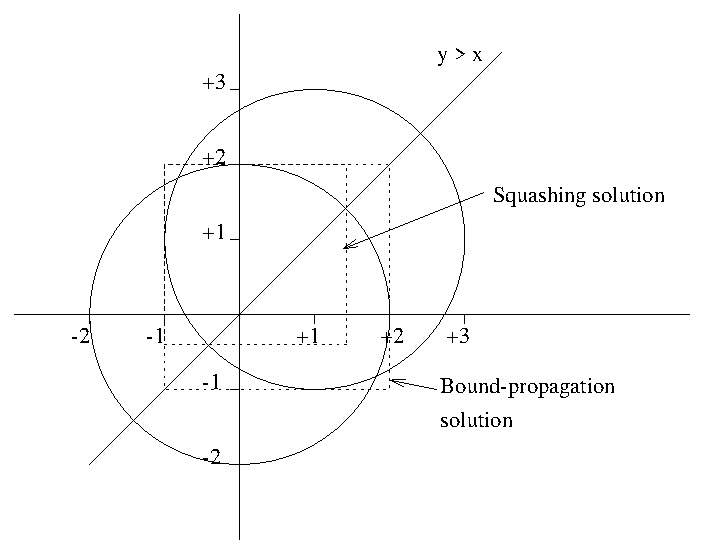
\includegraphics{example1.eps}
\caption{Propagation with Squash algorithm (example)}
\end{figure}

All points (X,Y) Y $>$= X, lying within the intersection of 2 circles with
radius 2, one centred at (0,0) the other at (1,1).
\begin{quote}
\begin{verbatim}
[eclipse 2]: 4 $>= X^2 + Y^2, 4 $>= (X-1)^2+(Y-1)^2, Y $>= X.

Y = Y{-1.0000000000000004 .. 2.0000000000000004}
X = X{-1.0000000000000004 .. 2.0000000000000004}

Delayed goals:
    ...
yes.
\end{verbatim}
\end{quote}
The bound-consistency solution does not take into account the X $>$= Y
constraint. Intuitively this is because it passes through the corners
of the box denoting the solution to the problem of simply intersecting
the two circles.

\begin{quote}
\begin{verbatim}
[eclipse 2]: 4 $>= X^2 + Y^2, 4 $>= (X-1)^2+(Y-1)^2, Y $>= X,
                squash([X,Y], 1e-5, lin).

X = X{-1.0000000000000004 .. 1.4142135999632601}
Y = Y{-0.41421359996326 .. 2.0000000000000004}

Delayed goals:
    ...
yes.
\end{verbatim}
\end{quote}

\subsection{Obtaining Solver Statistics}

(Using the facilities described in this section requires importing the
\bipref{ic_kernel}{../bips/lib/ic_kernel/index.html} module.  Also, since
they depend on the internals of the IC library, the details presented here
are subject to change without notice.)

Often it is difficult to know where the solver spends its time.
The library has built-in counters which keep track of the number of times
various events occur:
\begin{description}
    \item[ic_lin_create]
	The number of linear constraints set up.
    \item[ic_lin_prop]
	The number of times a linear constraint is propagated.
    \item[ic_uni_prop/ic_bin_prop/ic_tern_prop]
	The number of times a non-linear (unary/binary/ternary) operator is
	propagated.
    \item[ic_split]
	The number of domain splits in locate/2,3,4.
    \item[ic_squash]
	The number of squash attempts in squash/3 or locate/4.
\end{description}

Users who wish to track activity within their own programs may (if they
wish) use the same mechanism.  New event types can be registered (see
below) and actions recorded by calling the
\biptxtrefni{ic\_event(Event)}{ic_event/1!ic_kernel}{../bips/lib/ic_kernel/ic_event-1.html}
\index{ic_event/1@\texttt{ic_event/1}!ic_kernel}
predicate.

The counters are controlled using the primitives:
\begin{description}
\item[\biptxtrefni{ic\_stat(on)}{ic_stat/1!ic_kernel}{../bips/lib/ic_kernel/ic_stat-1.html}]
\index{ic_stat/1@\texttt{ic_stat/1}!ic_kernel}
\item[\biptxtrefni{ic\_stat(off)}{ic_stat/1!ic_kernel}{../bips/lib/ic_kernel/ic_stat-1.html}]
Enables/disable collection of statistics.  Default is off.

\item[\biptxtrefni{ic\_stat(reset)}{ic_stat/1!ic_kernel}{../bips/lib/ic_kernel/ic_stat-1.html}]
Reset statistics counters.

\item[\biptxtrefni{ic\_stat(print)}{ic_stat/1!ic_kernel}{../bips/lib/ic_kernel/ic_stat-1.html}]
Print statistics counters to the standard output stream.

\item[\biptxtrefni{ic\_stat_get(-Stat)}{ic_stat_get/1!ic_kernel}{../bips/lib/ic_kernel/ic_stat_get-1.html}]
Returns a list of CounterName=CounterValue pairs, summarising the
computation since the last reset.

\item[\biptxtrefni{ic\_event(+Name)}{ic_event/1!ic_kernel}{../bips/lib/ic_kernel/ic_event-1.html}]
Records the fact that the named event has happened.

\item[\biptxtrefni{ic_stat\_register\_event(+Name,+Description)}{ic_stat_register_event/2!ic_kernel}{../bips/lib/ic_kernel/ic_stat_register_event-2.html}]
Registers a new event type and sets the counter to 0.  This allows
user-defined predicates to record their own events within the same
framework.

\end{description}


\section{General Guidelines for the Use of the IC library}
Whilst IC has been designed to provide a flexible, consistent and yet
powerful framework for many sorts of constraint satisfaction
problems, it can not be all things to all people.

There are circumstances under which IC will not propagate all possible
information, for reasons of efficiency.

It is the purpose of this section to point out ways that may help IC
to solve problems more efficiently.

Typical constraint satisfaction problems are solved by iteratively
propagating information from basic constraints until no more
propagation can take place (i.e.\ a fixed point has been reached), and
then reducing the domain of a variable so as to prompt more
propagation.

As with most constraint solvers the propagation provided by the
builtin constraints is rarely able to solve large problems completely
without the need for some form of search.  A number of factors affect
the speed of the propagation phase.

\begin{enumerate}
\item The size of the initial domains.
Smaller domains typically result in propagation reaching a fixed point
sooner.  So give explicit initial domains to as many variables as possible.
\item Integer domains allow more propagation.
An important point to note here is that (as in mathematics) IC treats
integers as a strict subset of the reals, and as such the integer
domain \verb|0 .. 100| contains significantly fewer values than the
real domain \verb|0.0 .. 100.0|.  With this in mind, IC attempts to
infer integrality where possible (e.g.\ the sum of two integer variables
is constrained to be integer), however integer domains (where
applicable) should be used in user code.

The difference becomes apparent when dealing with strict inequalities, for example.
\begin{verbatim}
[eclipse 4]: reals([X]), X $> 5.

X = X{5.0 .. 1.0Inf}


Delayed goals:
        ic : (X{5.0 .. 1.0Inf} > 5)
Yes (0.00s cpu)
\end{verbatim}
Note that the lower bound of X is still five despite the fact that X
has been constrained to be strictly greater than five.  Further note
the presence of a delayed goal which will fail should X be constrained
to be exactly five.

\begin{verbatim}
[eclipse 5]: integers([X]), X $> 5.

X = X{6 .. 1.0Inf}
Yes (0.00s cpu)
\end{verbatim}
In this example since X is known to be integral, the lower bound of X
can be set to 6, as there are no integers between five and six.
\end{enumerate}


\section{User defined constraints}

The library \bipref{ic_kernel}{../bips/lib/ic_kernel/index.html} provides a
number of facilities useful for implementing IC constraints or otherwise
extending the facilities provided by the standard IC library.

While the \bipref{ic_kernel}{../bips/lib/ic_kernel/index.html} library
exposes the structure of the IC attribute to the programmer (see below),
accessing it directly is strongly discouraged (if for no other reason,
the internals of IC may continue to evolve).
For accessing information about a variable and its domain, use the
predicates described earlier in section~\ref{domain-query} ``Variable query
predicates''.
For modifying a variable, it is particularly important to go through the
access predicates, in order to make sure that the internal state remains
consistent, that appropriate constraints are scheduled for execution as a
result of the change, etc.
The predicates available for modifying a variable are discussed in the next
section.

\subsection{Modifying variable domains}

When using IC variables in normal code, one would typically use the
\verb|$\=|, \verb|$=<| and \verb|$>=| family of constraints to (resp.)
remove a value, reduce the upper bound or increase the lower bound of a
variable.

While these constraints are good for normal CSP solving, they have a
number of properties which may be less desirable when writing new
constraints.  In particular, they may leave unwanted delayed goals
behind and may perform extra propagation before returning (it may be
desirable to perform all required bound updates before allowing further
propagation to occur).

To give the constraint writer more control over such matters, special
predicates exist in the \bipref{ic_kernel}{../bips/lib/ic_kernel/index.html}
module which allow direct modification of the domain without the waking of
goals (they are scheduled for execution but not actually executed).
These predicates generally accept an IC variable, a non-IC variable (which
will be constrained to make it a real IC variable) or a number.

Full details on these predicates can be found in the reference manual; they
are listed here for completeness.  Note that with the exception of
\bipref{impose_bounds/3}{../bips/lib/ic_kernel/impose_bounds-3.html} none of
the goals call \bipref{wake/0}{../bips/kernel/suspensions/wake-0.html}, so
the programmer is free to do so at a convenient time.

\begin{description}
\item[\bipref{impose_min/2}{../bips/lib/ic_kernel/impose_min-2.html}]
Set the lowerbound.
\item[\bipref{impose_max/2}{../bips/lib/ic_kernel/impose_max-2.html}]
Set the upperbound.
\item[\bipref{impose_bounds/3}{../bips/lib/ic_kernel/impose_bounds-3.html}]
Sets both upper and lower bounds.
\item[\bipref{exclude/2}{../bips/lib/ic_kernel/exclude-2.html}]
Excludes an integer from an integral variable.
\item[\bipref{exclude_range/3}{../bips/lib/ic_kernel/exclude_range-3.html}]
Excludes a range of integers from an integral variable.
\item[\bipref{set_var_type/2}{../bips/lib/ic_kernel/set_var_type-2.html}]
Makes the variable be of the given type.
\item[\bipref{set_vars_type/2}{../bips/lib/ic_kernel/set_vars_type-2.html}]
Like set_var_type, but works for lists and submatrices of variables as well.
\end{description}

\subsection{The IC attribute}

The IC attribute is a meta-term which is attached to all variables which
take part in IC constraints.
\bipref{ic_kernel}{../bips/lib/ic_kernel/index.html} defines the IC
attribute as a structure of the following form:
\begin{verbatim}
ic{var_type:Type,
         lo:Lo,
         hi:Hi,
         bitmap:Bitmap,
         min:SuspMin,
         max:SuspMax,
         hole:SuspHole,
         type:SuspType
        }
\end{verbatim}


This structure holds:

\begin{description}
\item[var_type] The type of the variable.  This defaults to 'real' but may
become 'integer' after an explicit call to {\bf integers/1}, by being
included in an integer constraint (e.g.\ {\bf \#=}) or by inferences made
during constraint propagation.
\item[lo] The lower bound of the variable's domain, as a float.
\item[hi] The lower bound of the variable's domain, as a float.
\item[bitmap] Where relevant, a bitmap representation of the integer domain;
where not relevant it holds the atom \verb|undefined|.
\item[min] Suspension list of goals to be woken on lower bound changes.
\item[max] Suspension list of goals to be woken on upper bound changes.
\item[hole] Suspension list of goals to be woken when a value is removed
from the middle of a domain.  Such removals only happen for integer
variables whose domain is finite.
\item[type] Suspension list of goals to be woken when a variable's type
becomes more constrained, i.e.\ when a variable goes from being real to
being integer.
\end{description}

The suspension list names can be used in
\bipref{suspend/3}{../bips/kernel/suspensions/suspend-3.html} and
related predicates to denote an appropriate waking condition.

The attribute of a domain variable can be accessed with the predicate
\bipref{get_ic_attr/2}{../bips/lib/ic_kernel/get_ic_attr-2.html}.

As noted above, direct access and manipulation of the attribute is
discouraged; use the access predicates instead.

\index{library!ic|)}

%HEVEA\cutend



% BEGIN LICENSE BLOCK
% Version: CMPL 1.1
%
% The contents of this file are subject to the Cisco-style Mozilla Public
% License Version 1.1 (the "License"); you may not use this file except
% in compliance with the License.  You may obtain a copy of the License
% at www.eclipse-clp.org/license.
% 
% Software distributed under the License is distributed on an "AS IS"
% basis, WITHOUT WARRANTY OF ANY KIND, either express or implied.  See
% the License for the specific language governing rights and limitations
% under the License. 
% 
% The Original Code is  The ECLiPSe Constraint Logic Programming System. 
% The Initial Developer of the Original Code is  Cisco Systems, Inc. 
% Portions created by the Initial Developer are
% Copyright (C) 2006 Cisco Systems, Inc.  All Rights Reserved.
% 
% Contributor(s): Joachim Schimpf, IC-Parc
% 
% END LICENSE BLOCK
%
% $Id: fdglobal.tex,v 1.3 2015/10/16 17:28:39 kish_shen Exp $
%
% Author: Joachim Schimpf
%

\chapter{Global Finite Domain Constraints}
\label{chapglobconstr}
%HEVEA\cutdef[1]{section}
\section{Various Constraints over Lists and Arrays}

The libraries
\biptxtref{ic_global}{library(ic_global)}{../bips/lib/ic_global/index.html}
and
\biptxtref{ic_global_gac}{library(ic_global_gac)}{../bips/lib_public/ic_global_gac/index.html}
implement a number of constraints over lists of integer variables.
They are loaded using a directive like
\begin{quote}\begin{verbatim}
:- use_module(library(ic_global)).	% or :- lib(ic_global).
\end{verbatim}\end{quote}
For details of the implemented constraints, refer to the Reference Manual
for the libraries.

These constraints are commonly known as \aboutidx{global constraints},
which simply indicates that they can constrain a large number of variables
at once, without breaking up the constraint into more primitive constraints.
This can on one hand facilitate problem modelling, and on the other hand
lead to more effective constraint propagation.

Note that some constraints are implemented in both of the libraries:
in these cases, ic_global_gac implements a "globally arc consistent"
version, while ic_global implements a less computationally expensive
version with weaker propagation.

Among the constraints provided are the following (refer to the
Reference Manual for the complete list):

\begin{description}
\item[\biptxtref{alldifferent(+List)}{ic_global:alldifferent/1}{../bips/lib/ic_global/alldifferent-1.html}]\ \\
\index{alldifferent/1}
A version of alldifferent/1 with strong propagation.

\item[\biptxtref{alldifferent(+List, ++Capacity)}{ic_global:alldifferent/2}{../bips/lib/ic_global/alldifferent-2.html}]\ \\
\index{alldifferent/2}
Like alldifferent/1, but every value may occur Capacity times.

\item[\biptxtref{alldifferent_matrix(+Matrix)}{alldifferent_matrix/1}{../bips/lib/ic_global/alldifferent_matrix-1.html}]\ \\
Constrains the rows and columns of Matrix to be different values.

\item[\biptxtref{gcc(++Bounds,+Vars)}{gcc/2}{../bips/lib/gfd/gcc-2.html}]\ \\
The \aboutidx{global cardinality constraint} makes sure certain values
occur with a certain frequency in Vars.  This is a generalisation of the
occurrences-constraint.
See also \bipref{gcc_matrix/3}{../bips/lib_public/fd_global_gac/gcc_matrix-3.html}.

\item[\biptxtref{inverse(+Succ, +Pred)}{inverse/2}{../bips/lib/ic_global/inverse-2.html}]\ \\
Constrains elements of Succ to be the successors and Pred to be the
predecessors of nodes in a digraph.

\item[\biptxtref{lex_le(+List1, +List2)}{lex_le/2}{../bips/lib/ic_global/lex_le-2.html}]\ \\
\index{lexico_le/2}
Imposes a lexicographic ordering between the two lists.

\item[\biptxtref{lex_lt(+List1, +List2)}{lex_lt/2}{../bips/lib/ic_global/lex_lt-2.html}]\ \\
Imposes a strict lexicographic ordering between the two lists.

\item[\biptxtref{ordered(++Relation, +List)}{ordered/2}{../bips/lib/ic_global/ordered-2.html}]\ \\
\index{ordered/2}
Constrains List to be ordered according to Relation.
Relation is one of the atoms \lt, =\lt, \gt, \gt=, = .

\item[\biptxtref{ordered_sum(++List, +Sum)}{ordered_sum/2}{../bips/lib/ic_global/ordered_sum-2.html}]\ \\
\index{ordered_sum/2}
The list elements are ordered and their sum is Sum.  A combination of
ordered and sum constraint with stronger propagation.

\item[\biptxtref{occurrences(++Value, +List, ?N)}{occurrences/3}{../bips/lib/ic_global/occurrences-3.html}]\ \\
\index{occurrences/3}
The value Value occurs in List N times.
Operationally: N gets updated to reflect the number of
possible occurrences in the List. List elements may get
instantiated to Value, or Value may be removed from their
domain if required by N.

\item[\biptxtref{same(+List1, +List2)}{same/2}{../bips/lib_public/fd_global_gac/same-2.html}]\ \\
List2 is a permutation of List1.

\item[\biptxtref{sequence(+Low, +High, +K, +Vars, ++Values)}{sequence/5}{../bips/lib/gfd/sequence-5.html}]\ \\
Every subsequence of Vars of length K contains at least Low and at most High
occurrences of Values.
Also \bipref{sequence/4}{../bips/lib/gfd/sequence-4.html}.

\item[\biptxtref{sorted(?List, ?Sorted)}{ic_global:sorted/2}{../bips/lib/ic_global/sorted-2.html}]\ \\
\index{sorted/2}
Sorted is a sorted permutation of List.

\item[\biptxtref{sorted(?List, ?Sorted, ?Positions)}{ic_global:sorted/3}{../bips/lib/ic_global/sorted-3.html}]\ \\
\index{sorted/3}
Sorted is a sorted permutation of List and Positions is a list whose
elements indicating the position of each unsorted list element within
the sorted list.

\item[\biptxtref{sumlist(+List, ?Sum)}{ic_global:sumlist/2}{../bips/lib/ic_global/sumlist-2.html}]\ \\
\index{sumlist/2}
The sum of the list elements is Sum. This constraint
is more efficient than a general IC sum constraint
if the list is long and Sum is not constrained frequently.

\end{description}


\section{Cumulative Constraint and Resource Profiles}

The library {\bf cumulative} implements the cumulative scheduling constraint.
It is based on the IC library and is loaded using one of 
\begin{quote}\begin{verbatim}
:- use_module(library(ic_cumulative)).
:- lib(ic_cumulative).
\end{verbatim}\end{quote}


\begin{description}
\item[\biptxtref{cumulative(+StartTimes, +Durations, +Resources, ++ResourceLimit)}{ic_cumulative:cumulative/4}{../bips/lib/ic_cumulative/cumulative-4.html}]\ \\
\index{cumulative/4}
A cumulative scheduling constraint. StartTimes, Durations and Resources
are lists of equal length N of integer variables or integers.
ResourceLimit is an integer. The declarative meaning is:
If there are N tasks, each starting at a certain start time, having
a certain duration and consuming a certain (constant) amount of
resource, then the sum of resource usage of all the tasks does not
exceed ResourceLimit at any time.

\item[\biptxtref{profile(+StartTimes, +Durations, +Resources, -Profile)}{ic_cumulative:profile/4}{../bips/lib/ic_cumulative/profile-4.html}]\ \\
\index{profile/4}
StartTimes, Durations, Resources and Profile
are lists of equal length N of integer variables or integers
with the same meaning as in cumulative/4.
The list Profile indicates the level of resource usage at the
starting point of each task.
\end{description}


\section{Edge-finder}

The libraries {\bf ic_edge_finder} and {\bf ic_edge_finder3}
implement stronger versions of the
disjunctive and cumulative scheduling constraints. They employ
a technique known as edge-finding to derive stronger bounds on
the starting times of the tasks.
The library is loaded using either
\begin{quote}\begin{verbatim}
:- use_module(library(ic_edge_finder)).
\end{verbatim}\end{quote}
to get a weaker variant with quadratic complexity, or
\begin{quote}\begin{verbatim}
:- use_module(library(ic_edge_finder3)).
\end{verbatim}\end{quote}
to get a stronger variant with cubic complexity.

\begin{description}
\item[disjunctive(+StartTimes,+Durations)]\ \\
\index{disjunctive/2}
A disjunctive scheduling constraint. StartTimes and Durations
are lists of equal length N of integer variables or integers.
The declarative meaning is that the N tasks with certain start times
and duration do not overlap at any point in time.

\item[cumulative(+StartTimes,+Durations,+Resources,++ResourceLimit)]\ \\
\index{cumulative/4}
A cumulative scheduling constraint. StartTimes, Durations and Resources
are lists of equal length N of integer variables or integers.
ResourceLimit is an integer. The declarative meaning is:
If there are N tasks, each starting at a certain start time, having
a certain duration and consuming a certain (constant) amount of
resource, then the sum of resource usage of all the tasks does not
exceed ResourceLimit at any time.
This constraint can propagate more information than the implementation
in library(cumulative).

\item[cumulative(+StartTimes,+Durations,+Resources,+Area,++ResourceLimit)]\ \\
\index{cumulative/5}
In this variant, an area (the product of duration and resource usage of
a task) can be specified, e.g.\ if duration or resource usage are not
known in advance. The edge-finder algorithm can make use of this information
to derive bound updates.
\end{description}
%HEVEA\cutend

% BEGIN LICENSE BLOCK
% Version: CMPL 1.1
%
% The contents of this file are subject to the Cisco-style Mozilla Public
% License Version 1.1 (the "License"); you may not use this file except
% in compliance with the License.  You may obtain a copy of the License
% at www.eclipse-clp.org/license.
% 
% Software distributed under the License is distributed on an "AS IS"
% basis, WITHOUT WARRANTY OF ANY KIND, either express or implied.  See
% the License for the specific language governing rights and limitations
% under the License. 
% 
% The Original Code is  The ECLiPSe Constraint Logic Programming System. 
% The Initial Developer of the Original Code is  Cisco Systems, Inc. 
% Portions created by the Initial Developer are
% Copyright (C) 2006 Cisco Systems, Inc.  All Rights Reserved.
% 
% Contributor(s): 
% 
% END LICENSE BLOCK

%----------------------------------------------------------------------
\chapter{The Integer Sets Library}
%HEVEA\cutdef[1]{section}
\label{chapfdsets}
\index{library!fd_sets|(}
%----------------------------------------------------------------------


%----------------------------------------------------------------------
%\section{Introduction}
%----------------------------------------------------------------------

The {\em fd_sets} library is a solver for constraints over the domain
of finite sets of integers. Unlike {\em conjunto}, it cannot deal with
sets elements that are not integers. On the other hand, fd_sets is usually
faster for integer sets than conjunto.



\section{Ground Integer Sets}

(Ground) integer sets are simply sorted, duplicate-free lists of integers e.g. 
\begin{verbatim}
        SetOfThree = [1,3,7]
        EmptySet = []
\end{verbatim}
Lists which contain non-integers, are unsorted or contain duplicates,
are not sets in the sense of this library.


%----------------------------------------------------------------------
\section{Set Variables}
%----------------------------------------------------------------------

\subsection{Declaring}
Set variables are variables which can eventually take a ground integer
set as their value.  They are characterized by a lower bound (the set
of elements that are definitely in the set) and an upper bound (the
set of elements that may be in the set).  A set variable can be
declared as follows: 
\begin{verbatim}
        SetVar :: []..[1,2,3,4,5,6,7]
\end{verbatim}
If the lower bound is the empty set (like in this case) this can be written as 
\begin{verbatim}
        SetVar subset [1,2,3,4,5,6,7]
\end{verbatim}
If the lower bound is the empty set and the upper bound is a set of
consecutive integers, one can also declare it like
\begin{verbatim}
        intset(SetVar, 1, 7)
\end{verbatim}
which is equivalent to the above.    

The predicates to declare sets are:
\begin{description}
\item[\biptxtrefni{?Set :: ++Lwb..++Upb}{::/2!fd_sets}{../bips/lib/fd_sets/NN-2.html}]
\index{\::/2@\texttt{::/2}!fd_sets}
         Set is an integer set within the given bounds 
\item[\biptxtref{intset(?Set, +Min, +Max)}{intset/3}{../bips/lib/fd_sets/intset-3.html}]
         Set is a set containing numbers between Min and Max 
\item[\biptxtref{intsets(?Sets, ?N, +Min, +Max)}{intsets/4}{../bips/lib/fd_sets/intsets-4.html}]
         Sets is a list of N sets containing numbers between Min and Max 
\end{description}



\subsection{Printing}

Set variables are by default printed in a particular way, e.g.
\begin{verbatim}
?- X :: [2,3]..[1,2,3,4], write(X).
X{[2, 3] \/ ([] .. [1, 4]) : _308{[2 .. 4]}}
\end{verbatim}
The curly brackets contain
\begin{enumerate}
\item the lower bound of the set
\item the union symbol
\item the set of optional values (that may or may not be in the set)
\item a colon
\item a finite domain indicating the admissible cardinality for the set
\end{enumerate}



\subsection{Domain Access}

\begin{description}
\item[\biptxtref{potential_members(?Set, -List)}{potential_members/2}{../bips/lib/fd_sets/potential_members-2.html}]
         List is the list of elements of whose membership in Set is currently uncertain 
\item[\biptxtref{set_range(?Set, -Lwb, -Upb)}{set_range/3}{../bips/lib/fd_sets/set_range-3.html}]
         Lwb and Upb are the current lower and upper bounds on Set 
\end{description}


%----------------------------------------------------------------------
\section{Constraints}
%----------------------------------------------------------------------

\subsection{Membership}

\begin{description}
\item[\biptxtrefni{?X in ?Set}{in/2!fd_sets}{../bips/lib/fd_sets/in-2.html}]
\index{in/2@\texttt{in/2}!fd_sets}
         The integer X is member of the integer set Set 
\item[\biptxtrefni{?X notin ?Set}{notin/2!fd_sets}{../bips/lib/fd_sets/notin-2.html}]
\index{notin/2@\texttt{notin/2}!fd_sets}
         The integer X is not a member of the integer set Set 
\item[\biptxtrefni{membership_booleans(?Set, ?BoolArr)}{membership_booleans/2!fd_sets}{../bips/lib/fd_sets/membership_booleans-2.html}]
\index{membership_booleans/2@\texttt{membership_booleans/2}!fd_sets}
         BoolArr is an array of booleans describing Set 
\end{description}


\subsection{Cardinality}

\begin{description}
\item[\biptxtrefni{\#(?Set, ?Card)}{\#/2!fd_sets}{../bips/lib/fd_sets/H-2.html}]
\index{\#/2@\texttt{\#/2}!fd_sets}
         Card is the cardinality of the integer set Set 
\end{description}


\subsection{Set Relations}

\begin{description}

\item[\biptxtrefni{difference(?Set1, ?Set2, ?Set3)}{difference/3!fd_sets}{../bips/lib/fd_sets/difference-3.html}]
\index{difference/3@\texttt{difference/3}!fd_sets}
         Set3 is the difference of the integer sets Set1 and Set2 

\item[\biptxtrefni{?Set1 disjoint ?Set2}{disjoint/2!fd_sets}{../bips/lib/fd_sets/disjoint-2.html}]
\index{disjoint/2@\texttt{disjoint/2}!fd_sets}
         The integer sets Set1 and Set2 are disjoint 

\item[\biptxtrefni{?Set1 includes ?Set2}{includes/2!fd_sets}{../bips/lib/fd_sets/includes-2.html}]
\index{includes/2@\texttt{includes/2}!fd_sets}
         Set1 includes (is a superset) of the integer set Set2 

\item[\biptxtrefni{intersection(?Set1, ?Set2, ?Set3)}{intersection/3!fd_sets}{../bips/lib/fd_sets/intersection-3.html}]
\index{intersection/3@\texttt{intersection/3}!fd_sets}
         Set3 is the intersection of the integer sets Set1 and Set2 

\item[\biptxtrefni{?Set1 sameset ?Set2}{sameset/2!fd_sets}{../bips/lib/fd_sets/sameset-2.html}]
\index{sameset/2@\texttt{sameset/2}!fd_sets}
         The sets Set1 and Set2 are equal 
\item[\biptxtrefni{?Set1 subset ?Set2}{subset/2!fd_sets}{../bips/lib/fd_sets/subset-2.html}]
\index{subset/2@\texttt{subset/2}!fd_sets}
         Set1 is a subset of the integer set Set2 
\item[\biptxtrefni{symdiff(?Set1, ?Set2, ?Set3)}{symdiff/3!fd_sets}{../bips/lib/fd_sets/symdiff-3.html}]
\index{symdiff/2@\texttt{symdiff/2}!fd_sets}
         Set3 is the symmetric difference of the integer sets Set1 and Set2 
\item[\biptxtrefni{union(?Set1, ?Set2, ?Set3)}{union/3!fd_sets}{../bips/lib/fd_sets/union-3.html}]
\index{union/2@\texttt{union/2}!fd_sets}
         Set3 is the union of the integer sets Set1 and Set2 
\end{description}


\subsection{N-ary Set Relations}

\begin{description}
\item[\biptxtref{all_disjoint(+Sets)}{all_disjoint/1}{../bips/lib/fd_sets/all_disjoint-1.html}]
         Sets is a list of integers sets which are all disjoint 
\item[\biptxtref{all_union(+Sets, ?SetUnion)}{all_union/2}{../bips/lib/fd_sets/all_union-2.html}]
         SetUnion is the union of all the sets in the list Sets 
\item[\biptxtref{all_intersection(+Sets, ?SetIntersection)}{all_intersection/2}{../bips/lib/fd_sets/all_intersection-2.html}]
         SetIntersection is the intersection of all the sets in the list Sets 
\end{description}


\subsection{Set Weights}

\begin{description}
\item[\biptxtref{weight(?Set, ++ElementWeights, ?Weight)}{weight/3}{../bips/lib/fd_sets/weight-3.html}]
         According to the array of element weights, the weight of set Set1 is Weight 
\end{description}


%----------------------------------------------------------------------
\section{Set Expressions}
%----------------------------------------------------------------------

In most positions where a set or set variable is expected one can also
use a set expression. A set expression is composed from ground sets
(integer lists), set variables, and the following set operators:
\begin{verbatim}
    Set1 /\ Set2       % intersection
    Set1 \/ Set2       % union
    Set1 \ Set2        % difference
\end{verbatim}
When such set expressions occur, they are translated into auxiliary
\bipref{intersection/3}{../bips/lib/fd_sets/intersection-3.html},
\bipref{union/3}{../bips/lib/fd_sets/union-3.html} and
\bipref{difference/3}{../bips/lib/fd_sets/difference-3.html}
constraints, respectively.


%----------------------------------------------------------------------
\section{Search Support}
%----------------------------------------------------------------------

The
\bipref{insetdomain/4}{../bips/lib/fd_sets/insetdomain-4.html}
predicate can be used to enumerate all ground instantiations of a set
variable, much like
\bipref{indomain/1}{../bips/lib/fd/indomain-1.html}
in the finite-domain case. 

\begin{description}
\item[\biptxtref{insetdomain(?Set, ?CardSel, ?ElemSel, ?Order)}{insetdomain/4}{../bips/lib/fd_sets/insetdomain-4.html}]
         Instantiate Set to a possible value 
\end{description}


%----------------------------------------------------------------------
\section{Example}
%----------------------------------------------------------------------

The following program computes so-called Steiner triplets.
These are triplets of numbers from 1 to N such that
any two triplets have at most one element in common.
\begin{verbatim}
:- lib(fd_sets).
:- lib(fd).

steiner(N, Sets) :-
        NB is N * (N-1) // 6,           % compute number of triplets
        intsets(Sets, NB, 1, N),        % initialise the set variables
        ( foreach(S,Sets) do
            #(S,3)                      % constrain their cardinality
        ),
        ( fromto(Sets,[S1|Ss],Ss,[]) do
            ( foreach(S2,Ss), param(S1) do
                #(S1 /\ S2, C),         % constrain the cardinality
                C #<= 1                 % of pairwise intersections
            )
        ),
        label_sets(Sets).               % search

label_sets([]).
label_sets([S|Ss]) :-
        insetdomain(S,_,_,_),
        label_sets(Ss).
\end{verbatim}
Here is an example of running this program
\begin{verbatim}
?- steiner(9,X).

X = [[1, 2, 3], [1, 4, 5], [1, 6, 7], [1, 8, 9],
     [2, 4, 6], [2, 5, 8], [2, 7, 9], [3, 4, 9],
     [3, 5, 7], [3, 6, 8], [4, 7, 8], [5, 6, 9]] More? (;)
\end{verbatim}

\index{library!fd_sets|)}

%HEVEA\cutend


% BEGIN LICENSE BLOCK
% Version: CMPL 1.1
%
% The contents of this file are subject to the Cisco-style Mozilla Public
% License Version 1.1 (the "License"); you may not use this file except
% in compliance with the License.  You may obtain a copy of the License
% at www.eclipse-clp.org/license.
% 
% Software distributed under the License is distributed on an "AS IS"
% basis, WITHOUT WARRANTY OF ANY KIND, either express or implied.  See
% the License for the specific language governing rights and limitations
% under the License. 
% 
% The Original Code is  The ECLiPSe Constraint Logic Programming System. 
% The Initial Developer of the Original Code is  Cisco Systems, Inc. 
% Portions created by the Initial Developer are
% Copyright (C) 2006 Cisco Systems, Inc.  All Rights Reserved.
% 
% Contributor(s): 
% 
% END LICENSE BLOCK

%----------------------------------------------------------------------
\chapter{The Symbolic Domain Library}
%HEVEA\cutdef[1]{section}
\label{chapicsymbolic}
\index{library!ic_symbolic|(}
%----------------------------------------------------------------------


%----------------------------------------------------------------------
%\section{Introduction}
%----------------------------------------------------------------------

The {\em ic_symbolic} library is a solver for constraints over ordered
symbolic domains.
It is implemented on top of library(ic) (see \ref{chapic}),
by mapping symbolic domains to finite integer domains.
There are also several mixed-domain constraints, which have both
symbolic and integer arguments.

%----------------------------------------------------------------------
\section{Domains and Domain Variables}
%----------------------------------------------------------------------

This library uses the
\biptxtref{domain}{domain/1}{../bips/kernel/termcomp/domain-1.html}
feature provided by the ECLiPSe kernel. 
This means that domains need to be declared.
The declaration specifies the domain values and their order. For example:
\begin{quote}\begin{verbatim}
?- local domain(weekday(mo,tu,we,th,fr,sa,su)).
\end{verbatim}\end{quote}
declares a domain with name 'weekday' and values 'mo', 'tu' etc.  The
domain values are implicitly ordered, with 'mo' corresponding to 1,
until 'su' corresponding to 7.  Domain values must be unique within
one ECLiPSe module, i.e. a symbolic value can belong to at most one
domain.

A variable of a declared domain can then be created using
\begin{quote}\begin{verbatim}
?- X &:: weekday.
X = X{[mo, tu, we, th, fr, sa, su]}
Yes (0.00s cpu)
\end{verbatim}\end{quote}
or multiple variables using
\begin{quote}\begin{verbatim}
?- [X,Y,Z] &:: weekday.
X = X{[mo, tu, we, th, fr, sa, su]}
Y = Y{[mo, tu, we, th, fr, sa, su]}
Z = Z{[mo, tu, we, th, fr, sa, su]}
Yes (0.00s cpu)
\end{verbatim}\end{quote}


%----------------------------------------------------------------------
\section{Basic Constraints}
%----------------------------------------------------------------------
The following constraints implement the basic relationships between
two domain values.  The constraints require their arguments to come
from identical domains, otherwise an error is raised.
\begin{description}
\item[\biptxtrefni{?X \&= ?Y}{\&=/2!ic_symbolic}{../bips/lib/ic_symbolic/YE-2.html}]
\index{\&=/2@\texttt{\&=/2}!ic_symbolic}
    X is the same as Y
\item[\biprefnoidx{?X \&\bsl= ?Y}{../bips/lib/ic_symbolic/YRE-2.html}]
    \index{\&\bsl=/2!ic_symbolic}
    X is different from Y
\item[\biptxtrefni{?X \&$<$ ?Y}{\&</2!ic_symbolic}{../bips/lib/ic_symbolic/YL-2.html}]
\index{\&</2@\texttt{\&</2}!ic_symbolic}
    X is strictly before Y in the domain order
\item[\biptxtrefni{?X \&$>$ ?Y}{\&>/2!ic_symbolic}{../bips/lib/ic_symbolic/YG-2.html}]
    \index{\&>/2@\texttt{\&>/2}!ic_symbolic} X is strictly after Y in the domain order
\item[\biptxtrefni{?X \&=$<$ ?Y}{\&=</2!ic_symbolic}{../bips/lib/ic_symbolic/YEL-2.html}]
\index{\&=</2@\texttt{\&=</2}!ic_symbolic}
    X is the same as Y, or before Y in the domain order
\item[\biptxtrefni{?X \&$>$= ?Y}{\&>=/2!ic_symbolic}{../bips/lib/ic_symbolic/YGE-2.html}]
\index{\&>=/2@\texttt{\&>=/2}!ic_symbolic}
    X is the same as Y, or after Y in the domain order
\item[\biptxtrefni{shift(?X,?C,?Y)}{shift/1!ic_symbolic}{../bips/lib/ic_symbolic/shift-3.html}]
\index{shift/2@\texttt{shift/2}!ic_symbolic}
    Y is C places above X in the domain order.
    X and Y have symbolic domains, C has an integer domain.
\item[\biptxtrefni{rotate(?X,?C,?Y)}{rotate/3!ic_symbolic}{../bips/lib/ic_symbolic/rotate-3.html}]
\index{rotate/3@\texttt{rotate/3}!ic_symbolic}
    like shift/3 but wraps at domain boundary.
\item[\biptxtrefni{element(?Index,++List,?Value)}{element/3!ic_symbolic}{../bips/lib/ic_symbolic/element-3.html}]
\index{element/3@\texttt{element/3}!ic_symbolic}
    Value occurs in List at position Index.
    Value has a symbolic domain, Index has an integer domain.
    List is a number of symbolic domain values.
\end{description}
For example
\begin{quote}\begin{verbatim}
?- [X, Y] &:: weekday, X &< Y.
X = X{[mo, tu, we, th, fr, sa]}
Y = Y{[tu, we, th, fr, sa, su]}
Yes (0.00s cpu)

?- X &:: weekday, X &=< we.
X = X{[mo, tu, we]}
Yes (0.00s cpu)
\end{verbatim}\end{quote}
    

%----------------------------------------------------------------------
\section{Global Constraints}
%----------------------------------------------------------------------
A number of global constraints are available which directly correspond
(and are in fact implemented via) their counterparts in
lib(ic_global):
\begin{description}
\item[\biptxtrefni{alldifferent(+List)}{alldifferent/1!ic_symbolic}{../bips/lib/ic_symbolic/alldifferent-1.html}]
\index{alldifferent@\texttt{alldifferent}!ic_symbolic}
    All list elements are different
\item[\biptxtrefni{occurrences(++Value,+List,?N)}{occurrences/3!ic_symbolic}{../bips/lib/ic_symbolic/occurrences-3.html}]
    Value occurs N times in List
\item[\biptxtrefni{atmost(++N,+List,++Value)}{atmost/3!ic_symbolic}{../bips/lib/ic_symbolic/atmost-3.html}]
\index{atmost/3@\texttt{atmost/3}!ic_symbolic}
    Value occurs at most N times in List
\end{description}


%----------------------------------------------------------------------
\section{Internals}
%----------------------------------------------------------------------

Internally, symbolic domains are mapped to integer ranges from 1 up to
the number of domain elements.  The first value in the domain
declaration corresponds to 1, the second to 2 and so on.  Similarly,
symbolic domain variables can be mapped to a corresponding IC integer
variable.  This mapping is accessible through the predicate
\bipref{symbol_domain_index/3}{../bips/lib/ic_symbolic/symbol_domain_index-3.html}:
\begin{quote}\begin{verbatim}
?- symbol_domain_index(fr, D, I).
D = weekday
I = 5
Yes (0.00s cpu)

?- X &:: weekday, symbol_domain_index(X, D, I).
X = X{[mo, tu, we, th, fr, sa, su]}
D = weekday
I = I{1 .. 7}
Yes (0.00s cpu)

?- X &:: weekday, X &\= we, symbol_domain_index(X, D, I).
X = X{[mo, tu, th, fr, sa, su]}
D = weekday
I = I{[1, 2, 4 .. 7]}
Yes (0.00s cpu)
\end{verbatim}\end{quote}
    
The integer variable I mirrors the domain of the symbolic variable X and vice versa.

%----------------------------------------------------------------------
\section{Extending and Interfacing this Library}
%----------------------------------------------------------------------

Because of the mapping of symbols to integers, new constraints over
symbolic variables can be implemented simply by placing numeric (IC)
constraints on the corresponding integer variables.

Similarly, the facilities of the ic_search library can be exploited
when working with symbolic variables.  Instead of labeling the
symbolic variables, one can use the various facilities of ic_search to
label the corresponding integer variables instead.


%----------------------------------------------------------------------
\index{library!ic_symbolic|)}
%----------------------------------------------------------------------

%HEVEA\cutend


\chapter{GFD: Interface to Gecode Finite Domain Solver}
\label{chapgfd}
LIBRARY		"gfd.dll"
DESCRIPTION	"ECLiPSe Gecode Interface"
EXPORTS
	p_g_init			@1
        p_g_state_is_stable		@2
        p_g_check_handle		@3
        p_g_trail_undo_for_event	@4
	
	p_g_post_exclude_dom            @5
	p_g_post_exclude_dom_handle     @6
	p_g_post_exclude_val            @7
	p_g_post_exclude_range          @8
        p_g_post_interval		@9
        p_g_post_var_interval_reif	@10
        p_g_post_dom			@11
	p_g_post_dom_handle             @12
        p_g_post_var_dom_reif		@13
        p_g_post_var_val_reif		@14
        p_g_post_setvar			@15
        p_g_post_intrel_cstr		@16
        p_g_post_bool_connectives	@17
        p_g_post_alldiff		@18
        p_g_post_alldiff_offsets	@19
        p_g_post_count			@20
        p_g_post_gcc			@21
        p_g_post_element		@22
        p_g_post_sorted2		@23
        p_g_post_sorted			@24
        p_g_post_sequence		@25
        p_g_post_sequence_01		@26
        p_g_post_circuit		@27
        p_g_post_circuit_cost		@28
        p_g_post_disj			@29
        p_g_post_disjflex		@30
        p_g_post_cumulative		@31
        p_g_post_cumulativeflex		@32
        p_g_post_cumulatives		@33
	p_g_post_ordered		@34
	p_g_post_lex_order		@35
	p_g_post_bin_packing		@36	
        p_g_post_sum			@37
        p_g_post_lin			@38
        p_g_post_sum_reif		@39
        p_g_post_lin_reif		@40
        p_g_post_maxlist		@41
        p_g_post_minlist		@42
        p_g_post_sqrt			@43
        p_g_post_sq			@44
        p_g_post_abs			@45
        p_g_post_div			@46
        p_g_post_mult			@47
        p_g_post_mod			@48
        p_g_post_min2			@49
        p_g_post_max2			@50
        p_g_post_divmod			@51
        p_g_post_boolchannel		@52
        p_g_post_inverse		@53
        p_g_post_inverse_offset		@54
	p_g_post_ordered		@55
	p_g_post_lex_order		@56
        p_g_post_bin_packing		@57
        p_g_post_cumulative		@58
	p_g_post_rel			@59
	p_g_post_lwb			@60
	p_g_post_upb			@61
	p_g_post_nvalues		@62
	p_g_post_among			@63
	p_g_post_count_matches		@64
	p_g_post_ham_path		@65
	p_g_post_ham_path_cost		@66
	p_g_post_disjoint2		@67
	p_g_post_disjointflex2		@68
	p_g_post_collection_rel		@69
	p_g_post_precede		@70
	p_g_post_precede_chain		@71
	p_g_post_mem			@72
	p_g_post_mem_reif		@73
	p_g_post_table			@74
	p_g_post_extensional		@75
	p_g_post_exclude_var_val	@76
	p_g_post_simple_reif_rc		@77
	p_g_post_dom_var		@78
	p_g_post_minidx			@79
	p_g_post_maxidx			@80
	p_g_post_bin_packing_md		@81


        p_g_check_val_is_in_var_domain	@82
        p_g_get_var_bounds		@83
        p_g_get_var_value		@84
        p_g_get_var_domain		@85
        p_g_get_var_lwb			@86
        p_g_update_and_get_var_bound	@87
        p_g_get_var_upb			@88
        p_g_get_var_domain_size		@89
        p_g_get_var_domain_width	@90
        p_g_get_var_degree		@91
        p_g_get_var_median		@92
        p_g_get_var_afc			@93
        p_g_get_var_regret_lwb		@94
        p_g_get_var_regret_upb		@95
        p_g_setup_search		@96
        p_g_do_search			@97
        p_g_get_gfd_maxint		@98
        p_g_get_gfd_minint		@99
        p_g_add_newvars_dom_union	@100
        p_g_get_var_domain_handle	@101
        p_g_add_newvar_copy		@102
	p_g_link_newbools		@103
        p_g_propagate			@104
        p_g_propagate_recompute		@105
	p_g_stop_caching		@106
	p_g_start_caching		@107
	p_g_create_tupleset_handle	@108
	p_g_create_regdfa_handle	@109
	p_g_create_dfa_handle		@110
        p_g_add_newbool			@111
        p_g_add_newvars_interval	@112
        p_g_add_newvars_dom		@113
	p_g_add_newvars_as_bool		@114
	p_g_add_newvars_dom_handle      @115
	p_g_create_select_handle        @116
	p_g_select			@117
        p_g_create_ldsbsyms_handle	@118
        p_g_add_ldsbsym_valueinter	@119
        p_g_add_ldsbsym_variableinter	@120
        p_g_add_ldsbsym_parvalueinter	@121
        p_g_add_ldsbsym_parvariableinter @122
        p_g_add_ldsbsym_valuesreflect	@123
        p_g_add_matrix_ldsbsym		@124
	p_g_set_afc_decay		@125
	p_g_get_afc_decay		@126
	p_g_reset_afc			@127
	p_g_get_propagator_num		@128
        p_g_delete			@129
	p_g_init_space_handle_c		@130

	p_g_gecode_version		@131


% BEGIN LICENSE BLOCK
% Version: CMPL 1.1
%
% The contents of this file are subject to the Cisco-style Mozilla Public
% License Version 1.1 (the "License"); you may not use this file except
% in compliance with the License.  You may obtain a copy of the License
% at www.eclipse-clp.org/license.
% 
% Software distributed under the License is distributed on an "AS IS"
% basis, WITHOUT WARRANTY OF ANY KIND, either express or implied.  See
% the License for the specific language governing rights and limitations
% under the License. 
% 
% The Original Code is  The ECLiPSe Constraint Logic Programming System. 
% The Initial Developer of the Original Code is  Cisco Systems, Inc. 
% Portions created by the Initial Developer are
% Copyright (C) 1999 - 2006 Cisco Systems, Inc.  All Rights Reserved.
% 
% Contributor(s): Mark Wallace, IC-Parc
% 
% END LICENSE BLOCK

%
% @(#)extpropia.tex	2.0 23/02/99 
%
% Author: Mark Wallace
%
%\documentstyle{report}
%\begin{document}
\chapter{Propia - A Library Supporting Generalised Propagation}
%HEVEA\cutdef[1]{section}
\label{chappropia}

\label{Propia}
\index{Propia}
\section{Overview}

Propia is the name for the implementation of Generalised Propagation in
\eclipse.
  
Generalised propagation is {\em not} restricted
to integer domains, but can be applied to any goal the user cares to specify
even if the variables don't have domains.

Effectively the system looks ahead to determine if 
an approximation to the possible answers has a non-trivial generalization.
It is non-trivial if it enables any variables in the goal to become
further instantiated, thus reducing search.  

The background and motivation for Generalised Propagation is given in
references \cite{LeProvost92,LeProvost92a,LeProvost93b}.  This section
focusses on how to use it.  Further examples of the use of Propia are
distributed with \eclipse in the \verb+doc/examples/propia/+ directory
.  A simple demonstration of Propia in action on Lewis Carroll's Zebra
problem can be run by compiling \verb0zebra.pl0 and issuing the query
\verb+lib(ic), zebra(Houses,ic)+ .  An slightly more complex
application of Propia to crossword generation can be run by compiling
\verb0crossword0.


\index{infers}
Using Propia it is easy to take a standard Prolog program and, with
minimal syntactic change, to turn it into a constraint logic program.
Any goal \verb0Goal0 in the Prolog program, can be transformed into a
constraint by annotating it thus \verb0Goal infers most0.
The resulting constraint admits just the same answers as
the original goal, but its behaviour is quite different.
Instead of evaluating the goal by non-deterministically selecting
a clause in its definition and evaluating the clause body, Propia
evaluates the resulting constraint by extracting information from it
deterministically.
Propia extracts as much information as possible from the constraints
before selecting an ordinary Prolog goal and evaluating it.  In this
way Propia reduces the number of choices that need to be explored and
thus makes programs more efficient.

\section{Invoking and Using Propia}

Propia is an \eclipse library, loaded by calling
\begin{quote}
\begin{verbatim}
?- lib(propia).
\end{verbatim}
\end{quote}
A goal, such as \verb0member(X,[1,2,3])0, is turned into a constraint
by annotating it using the \verb0infers0 operator.
The second argument of \verb0infers0 defines how much propagation
should be attempted on the constraint and will be described in
section \ref{approx} below. 
In this section we shall use \verb0Goal infers most0, which infers as
much information as possible, given the loaded constraint solvers.  If
the \verb+IC+ solver is loaded, then \verb+IC+ information is
extracted, and Propia reduces the domains to achieve arc-consistency.

We first show the behaviour of the original goal:
\begin{quote}
\begin{verbatim}
?- member(X, [1, 2, 3]).
X = 1
Yes (0.00s cpu, solution 1, maybe more)
X = 2
Yes (0.02s cpu, solution 2, maybe more)
X = 3
Yes (0.02s cpu, solution 3)
\end{verbatim}
\end{quote}
\index{most}
Constraint propagation is invoked by \verb0infers most0:
\begin{quote}
\begin{verbatim}
?- lib(ic).
...
?- member(X, [1, 2, 3]) infers most.
X = X{1 .. 3}
Yes (0.00s cpu)
\end{verbatim}
\end{quote}
Note that the information produced by the constraint solves the
corresponding goal as well.
The constraint can thus be dropped.

In case there remains information not yet extracted, the constraint
must delay so that completeness is preserved:
\begin{quote}
\begin{verbatim}
?- member(X,Y) infers most.

X = X
Y = [H3|T3]
Delayed goals:
    member(X, [H3|T3]) infers most
yes.
\end{verbatim}
\end{quote}
Propia copes correctly with built-in predicates, such as \#\gt and
\#\lt, so after compiling this simple program:
\begin{quote}
\begin{verbatim}
notin3to6(X) :- X#<3.
notin3to6(X) :- X#>6.
\end{verbatim}
\end{quote}
the predicate can be used as a constraint:
\begin{quote}
\begin{verbatim}
?- X :: 1 .. 10, notin3to6(X) infers most.
X = X{[1, 2, 7 .. 10]}
Yes (0.00s cpu)
\end{verbatim}
\end{quote}
In this example there are no ``delayed'' constraints since all valuations for
{\em X} satisfying the above conditions are solutions.  Propia
detects this and therefore avoids delaying the constraint
again.

\index{scheduling}
\index{disjunctive constraints}
\index{constraints!disjunctive}
In scheduling
applications it is necessary to constrain two tasks that require the
same machine not to be performed at the same time.
Specifically one must end before the other begins, or vice versa.
If one task starting at time {\em ST1} has duration {\em D1} and another
task starting at time {\em ST2} has duration {\em D2}, the above
``disjunctive'' constraint is
expressed as follows:
\begin{quote}
\begin{verbatim}
noclash(ST1,D1,ST2,D2) :- ST1 #>= ST2+D2.
noclash(ST1,D1,ST2,D2) :- ST2 #>= ST1+D1.
\end{verbatim}
\end{quote}
Generalised Propagation on this constraint allows useful information
to be extracted even before it is decided in which order the tasks
should be run:
\begin{quote}
\begin{verbatim}
?- lib(ic).
...

?- [ST1, ST2] :: 1 .. 10, noclash(ST1, 5, ST2, 7) infers most.
ST1 = ST1{[1 .. 5, 8 .. 10]}
ST2 = ST2{[1 .. 3, 6 .. 10]}
There is 1 delayed goal.
Yes (0.00s cpu)
\end{verbatim}
\end{quote}
The values {\em 6} and {\em 7} are removed from the domain of {\em ST1} because
the goal \verb0noclash(ST1,5,ST2,7)0 cannot be satisfied if {\em ST1} is
either {\em 6} or {\em 7}.  For example if {\em ST1} is {\em 6}, then either 
$6>ST2+7$ (to satisfy the first clause defining \verb0noclash0)
or else $ST2>6+5$ (to satisfy the second clause).  There is no value for
$ST2 in \{1...10\}$ that makes either inequality true, and so {\em 6} is
removed from the domain of {\em ST1}.  By a similar reasoning
{\em 4} and {\em 5} are removed from the domain of {\em ST2}.

\index{propositional logic}
We next take a simple example from propositional logic.
In this example the result of constraint propagation is reflected not
only in the variable domains, but also in the unification of problem
variables.
We first define logical conjunction by its truth table:
\begin{quote}
\begin{verbatim}
land(true,true,true).
land(true,false,false).
land(false,true,false).
land(false,false,false).
\end{verbatim}
\end{quote}
Now we ask for an $X,Y,Z$ satisfying
$land(X,Y,Z) \wedge X=Y$.
Both solutions have $X=Y=Z$, and this information is produced solely
by propagating on the \verb0land0 constraint:
\begin{quote}
\begin{verbatim}
?- land(X, Y, Z) infers most, X = Y.
Z = X
X = X
Y = X
There is 1 delayed goal.
Yes (0.00s cpu)
\end{verbatim}
\end{quote}


\index{resource allocation}
We now illustrate the potential efficiency benefits of Generalised
Propagation with a simple resource allocation 
problem.  A company makes 9 products, each of which require two kinds
of components in their manufacture, and yields a certain profit.
This information is held in the following table.
\begin{quote}
\begin{verbatim}
/*** product(Name,#Component1,#Component2,Profit). **/
product(1,1,19,1).
product(2,2,17,2).
product(3,3,15,3).
product(4,4,13,4).
product(5,10,8,5).
product(6,16,4,4).
product(7,17,3,3).
product(8,18,2,2).
product(9,19,1,1).
\end{verbatim}
\end{quote}
We wish to find which products to manufacture in order to make a
certain profit without 
using more than a certain number of either kind of
component.\footnote{To keep the example simple there is no optimisation.}

We first define a predicate \verb0sum(Products,Comp1,Comp2,Profit)0
which relates a list of products (eg \verb0Products0=\verb0[1,5,1]0), 
to the number of each component required to build all the products in the list
and the profit
(for \verb0[1,5,1]0, \verb0Comp1=120 and \verb0Comp2=460 and
\verb0Profit=70).
\begin{quote}
\begin{verbatim}
sum([],0,0,0).
sum([Name|Products],Count1,Count2,Profit) :- 
    [Count1,Count2,Profit]::0..100,
    product(Name,Ct1a,Ct2a,Profita),
    Count1 #= Ct1a+Ct1b,
    Count2 #= Ct2a+Ct2b,
    Profit #= Profita+Profitb,
    sum(Products,Ct1b,Ct2b,Profitb).
\end{verbatim}
\end{quote}
If \verb0sum0 is invoked with a list of variables as its first argument,
eg \verb0[V1,V2,V3]0, then the only choice made during execution is at
the call to \verb0product0.  In short, for each variable in the input
list there are {\em 9} alternative products that could be chosen.
For a list of three variables there are consequently
$9^3= 729$
alternatives.

If we assume a production batch of {\em 9} units, then the number of
alternative ways of solving \verb0sum0 is
$9^9$
, or nearly 400
million.  To avoid exploring so many possibilities, we simply annotate
the call to \verb0product(Name,Ct1a,Ct2a,Profita)0 as a Generalised
Propagation constraint.
Thus the new definition of \verb0sum0 is:
\begin{quote}
\begin{verbatim}
sum([],0,0,0).
sum([Name|Products],Count1,Count2,Profit) :- 
    [Count1,Count2,Profit]::0..100,
    product(Name,Ct1a,Ct2a,Profita) infers most,
    Count1 #= Ct1a+Ct1b,
    Count2 #= Ct2a+Ct2b,
    Profit #= Profita+Profitb,
    sum(Products,Ct1b,Ct2b,Profitb).
\end{verbatim}
\end{quote}
Now \verb0sum0 refuses to make any choices:
\begin{quote}
\begin{verbatim}
?- sum([V1, V2, V3], Comp1, Comp2, Profit).
V1 = V1{1 .. 9}
V2 = V2{1 .. 9}
V3 = V3{1 .. 9}
Comp1 = Comp1{3 .. 57}
Comp2 = Comp2{3 .. 57}
Profit = Profit{3 .. 15}
There are 9 delayed goals.
Yes (0.01s cpu)
\end{verbatim}
\end{quote} 

Using the second version of \verb0sum0,
it is simple to write a program which produces lists of products
which use less than a given number \verb0Max10 and \verb0Max20 of each
component, and yields more than a given profit \verb0MinProfit0: 
\begin{quote}
\begin{verbatim} 
solve(Products,Batch,Max1,Max2,MinProfit) :-
    length(Products,Batch),
    Comp1 #=< Max1,
    Comp2 #=< Max2,
    Profit #>= MinProfit,
    sum(Products,Comp1,Comp2,Profit),
    labeling(Products).
\end{verbatim}
\end{quote}
The following query finds which products to manufacture in order to make a
profit of 40 without 
using more than 95 of either kind of component.
\begin{quote}
\begin{verbatim}
?- solve(P, 9, 95, 95, 40).
P = [1, 4, 5, 5, 5, 5, 5, 5, 5]
Yes (0.03s cpu, solution 1, maybe more)
\end{verbatim}
\end{quote}

Constraints can be dropped as soon
as they became redundant (i.e. as soon as they were entailed by the
current partial solution).
The check for entailment can be expensive, so Propia only drops
constraints if a simple syntactic check allows it.
For {\em infers most}, this check succeeds if the \verb+IC+
library is loaded, and the constraint has only one remaining variable.

\section{Approximate Generalised Propagation}
\label{approx}
\index{approximate generalised propagation}
\index{unique}
\index{consistent}

The syntax {\em Goal infers most} can also be varied to invoke
different levels of Generalised Propagation.  Other alternatives are
{\em Goal infers ic}, 
{\em Goal infers unique}, and {\em Goal infers consistent}.
The strongest constraint is generated by {\em Goal infers most},
but it can be expensive to compute.  The other alternatives may be
evaluated more efficiently, and may yield a better overall performance
on different applications.
We call them ``approximations'', since the information they produce
during propagation is a (weaker) approximation of the information
produced by the strongest constraint.

We illustrate the different approximations supported by the current
version of Propia on a single small example.
The results for {\em Goal infers most} reflect the problem that
structured terms cannot appear in \verb+IC+ integer domains.
\begin{quote}
\begin{verbatim} 
p(1,a).
p(2,f(Z)).
p(3,3).
\end{verbatim}

\begin{verbatim}
?- p(X, Y) infers most.
X = X{1 .. 3}
Y = Y
There is 1 delayed goal.
Yes (0.00s cpu)

?- X :: 1 .. 3, p(X, Y) infers most.
X = X{1 .. 3}
Y = Y
There is 1 delayed goal.
Yes (0.00s cpu)

?- p(2, Y) infers most.
Y = f(_326)
There is 1 delayed goal.
Yes (0.00s cpu)
\end{verbatim}
\end{quote} 
The first approximation we will introduce in this section 
is one that searches for the unique answer to
the query.
It is written {\em Goal infers unique}.
This is cheap because as soon as two different answers to the query
have been found, the constraint evaluation terminates and the
constraint is delayed again until new information becomes available.
Here are two examples of this approximation.
In the first example notice that no domain is produced for {\em X}.
\begin{quote}
\begin{verbatim}
?- p(X, Y) infers unique.
X = X
Y = Y
There is 1 delayed goal.
Yes (0.00s cpu)
\end{verbatim}
\end{quote}
In the second example, by contrast, \verb0infers unique0 yields the same
result as \verb0infers most0: 
\begin{quote}
\begin{verbatim} 
?- p(X,X) infers unique.
X = 3
Yes (0.00s cpu)
\end{verbatim}
\end{quote}

The next example shows that  {\em unique} can even capture
nonground answers:
\begin{quote}
\begin{verbatim}
?- p(2, X) infers unique.
X = f(Z)
Yes (0.00s cpu)
\end{verbatim}
\end{quote}

The next approximation we shall describe is even weaker: it tests if there is an
answer and if not it fails.
If there is an answer it checks to see if the constraint is already
true.

\begin{quote}
\begin{verbatim}
?- p(1, X) infers consistent.
X = X
There is 1 delayed goal.
Yes (0.00s cpu)

?- p(1, a) infers consistent.
Yes (0.00s cpu)

?- p(1, X) infers consistent, X = b.
No (0.00s cpu)
\end{verbatim}
\end{quote}

The strongest language \verb0infers most0 extracts any information
possible from the loaded constraint solvers.  The solvers currently
handled by Propia are {\em unification} (which is the built-in solver
of Prolog), {\em ic} and {\em ic_symbolic}.  The \verb+IC+ library is
loaded by \verb0lib(ic)0 and the symbolic library by
\verb0lib(ic_symbolic)0.  These libraries are described elsewhere.  If
both libraries are loaded, then \verb0infers most0 extracts
information from unification, \verb+IC+ domains and symbolic domains.  For example:
\begin{quote}
\begin{verbatim} 
 p(f(X),1) :- X *>=0, X *=< 10.
 p(f(X),1) :- X=12.
\end{verbatim}
\end{quote}
with the above program
\begin{quote}
\begin{verbatim} 
?- p(X, Y) infers most.
X = f(_338{0.0 .. 12.0})
Y = Y{[1, 2]}
There is 1 delayed goal.
Yes (0.00s cpu)
\end{verbatim}
\end{quote}

The approximation \verb0infers ic0 is
similar to \verb0infers most0.  However, while \verb0infers most0
extracts information based on whatever constraint solvers are loaded, 
the others only infers information derived from the specified constraint
solver.
Here's the same example using \verb0infers ic0:
\begin{quote}
\begin{verbatim} 
?- p(X, Y) infers ic.
X = f(_353{0.0 .. 12.0})
Y = Y{[1, 2]}
There is 1 delayed goal.
Yes (0.00s cpu)
\end{verbatim}
\end{quote}

One rather special approximation langue is \verb0infers ac0, where
\verb0ac0 stands for arc-consistency.
This has similar semantics to \verb0infers ic0, but is implemented
very efficiently using the built-in \verb0element0 constraint of the
\verb+IC+ solver.
The limitation is that \verb0Goal infers ac0 is implemented by
executing the goal repeatedly to find all the solutions, and then
manipulating the complete set of solutions.
It will only work in case there are finitely many solutions and they
are all ground.  


Finally it is possible to invoke Propia in such a way as to influence
its waking conditions.  To do this, use the standard
\verb0suspend0 syntax.  For example ``forward checking'' can be
implemented as follows:
\begin{quote}
\begin{verbatim}
propagate(Goal,fc) :- !,
    suspend(Goal,7,Goal->inst) infers most.
\end{verbatim}
\end{quote}
In this case the Propia constraint wakes up each time a variable in
the goal is instantiated.   

The default priority for
Propia constraints is $3$.
However, in the above example, the priority of the Propia
constraint has been set to $7$.

%HEVEA\cutend



% BEGIN LICENSE BLOCK
% Version: CMPL 1.1
%
% The contents of this file are subject to the Cisco-style Mozilla Public
% License Version 1.1 (the "License"); you may not use this file except
% in compliance with the License.  You may obtain a copy of the License
% at www.eclipse-clp.org/license.
% 
% Software distributed under the License is distributed on an "AS IS"
% basis, WITHOUT WARRANTY OF ANY KIND, either express or implied.  See
% the License for the specific language governing rights and limitations
% under the License. 
% 
% The Original Code is  The ECLiPSe Constraint Logic Programming System. 
% The Initial Developer of the Original Code is  Cisco Systems, Inc. 
% Portions created by the Initial Developer are
% Copyright (C) 1995 - 2006 Cisco Systems, Inc.  All Rights Reserved.
% 
% Contributor(s): Thom Fruehwirth & Pascal Brisset, ECRC
%                 Kish Shen, IC-Parc
% 
% END LICENSE BLOCK

%
% @(#)extchr.tex        1.16 95/05/29 
% Author:       Thom Fruehwirth & Pascal Brisset
%
%               Kish Shen 98/6/29
%                   Modified 2002-09-23
%               
%               Deleted sections on Opium (no longer in Eclipse), 
%               plus new sections on the new CHR library

\newcommand{\OU}{$|$~}

\newcommand{\rep}{{\tt <=>}\ }
\newcommand{\aug}{{\tt ==>}\ }
\newcommand{\rul}{{\tt :-}\ }


\chapter{The Constraint Handling Rules Library}
%HEVEA\cutdef[1]{section}
\label{chapchr}
\index{library!chr.pl|(}

%\date{931214}

The {\tt ech} library implements constraint handling rules
\index{constraint handling rules} (\chrs)\index{CHR@{\sf CHR}},
which can be mixed with normal \eclipse code.
%It includes a compiler, which translates \chr\ programs into
%\eclipse\ programs, and a runtime system.
%A second library ({\tt
%chr_opium.op}) is provided for the debugger which uses Opium, the
%high-level debugging environment of \eclipse.  
Several constraint handlers are
provided in example files in the directory {\tt ech}.

This library will replace the older {\tt chr} library. 
In addition, there is now an experimental extended implementation of {\chrs}. 
This extended implementation is faster than the existing {\tt chr} library,
and contains some extensions and changes. This is described in 
section~\ref{newchr}.

\section{Introduction}

{\em Constraint handling rules} (\chrs,
CHR home page \ahrefurl{\url{http://www.cs.kuleuven.ac.be/~dtai/projects/CHR/}})
\cite{fru92}
are a high-level language
extension to write {\em user-defined} constraints. \chrs\ 
consists of guarded rules with multiple heads.
%embedded in %a given host language (Prolog, Lisp, ML), in this case \eclipse.

The high-level \chrs\ are an excellent tool for {\em rapid prototyping} and
implementation of constraint handlers. The usual abstract formalism to
describe a constraint system, i.e. inference rules, rewrite rules,
sequents, formulas expressing axioms and theorems, can be written as
\chrs\ in a straightforward way.  Starting from this {\em executable
specification}, the rules can be refined and adapted
to the specifics of the application.  

\chrs\ define {\em simplification} of, and {\em propagation} over, 
user-defined constraints.  Simplification replaces constraints by
simpler constraints while preserving logical equivalence (e.g.  {\tt
X>Y,Y>X
\rep fail}).  Propagation adds new constraints which are logically
redundant but may cause further simplification (e.g. {\tt X>Y,Y>Z \aug
X>Z}).  Repeatedly applying \chrs\ incrementally simplifies and
finally solves user-defined constraints (e.g. {\tt A>B,B>C,C>A}
leads to {\tt fail}).  

With multiple heads and propagation rules,
\chrs\ provide two features which are essential for non-trivial
constraint handling.
%and which are not provided by any constraint
%logic programming language except CHIP \cite{chip}.  
%We can interpret constraints as a computationally efficient incarnation of predicates.
%Then \chrs\ have a declarative semantics. 
The declarative reading of
\chrs\ as formulas of first order logic 
allows one to reason about their correctness.  On the other hand, 
regarding \chrs\ as a rewrite system on logical formulas allows one to
reason about their termination and confluence.


In the next section
it is explained how to use \chrs.
 Then,
example constraint handlers and the colour graphic
demo are listed.
 The next
section introduces the basics of the \chr\ language and how it works.  
The next section describes more of the \chr\ language,
the section after the built-in labeling feature.
Then there is
a section on how to write good \chr\ programs.  Next the debuggers for
\chrs\ are introduced.  
%Last the Opium scenario for the Opium debugger
%is described.


\section{Using Constraint Handling Rules}

Here are the steps to be taken from writing to using \chrs:
\begin{itemize}
 \item Write a \chr\ program in a file 
File\verb/.chr/.

 \item In \eclipse, load the {\tt chr} library with the query
\verb/lib(chr)/. It contains both the compiler and runtime system for
\chrs. Now \eclipse\ is in coroutining mode.

 \item Compile your \verb/chr/ file into a \verb/pl/ file with the query
 \verb/chr2pl(/File\verb/)./

\item In any \eclipse\ session, you can load a compiled constraint handler
(\verb/[/File\verb/]./). The \chr\ library is automatically loaded
to provide the necessary runtime environment. \eclipse\ is in coroutining mode.

\end{itemize}
You can compile your \verb/chr/ file and load the resulting \verb/pl/ file
at once using the query \verb/chr(/File\verb/)./



\section{Example Constraint Handlers}

All example files are in the subdirectory {\tt lib/chr} of the
installation-directory of \eclipse\ (which can be found using {\tt
get\_flag(installation\_directory,Dir)}\index{constraint solvers}.  
The files ({\tt .chr, .pl}, examples)
relevant to a
particular constraint system can be found by looking at all files that
match the pattern given in the following listing with each example
handler.  The examples include a {\em colour graphic demo} about
optimal sender placement for wire-less devices in buildings and
company sites, small constraint handlers for
\begin{itemize}
%\item n-queens (no\_attack as constraint reduces backtracking),
\item minimum, maximum of and inequalities between terms ({\tt *minmax*})\index{minmax constraints},
\item terms ({\tt functor/3, arg/3, =..} as constraints) ({\tt *term*})\index{term constraints},
\item lists (similar to Prolog III) ({\tt *list*})\index{list constraints},
\item rational trees ({\tt *tree*})\index{tree constraints},
\item sound if-then-else, negation and checking, 
        lazy conjunction and disjunction ({\tt *control*})\index{control!sound},
\item geometric reasoning about rectangles ({\tt *demo*})\index{geometric constraints},
\end{itemize}
\noindent and larger constraint handlers for
\begin{itemize}
\item booleans for propositional logic ({\tt *bool*})\index{boolean constraints}\index{propositional logic},
\item finite and {\em infinite} domains (inspired by CHIP) ({\tt *domain*})\index{domain constraints},
\item sets ({\tt *set*})\index{set constraints},
\item terminological reasoning (similar to KL-ONE) \cite{fru93b} ({\tt *kl-one*})\index{terminological constraints},
\item temporal reasoning (over time points and intervals) \cite{fru93} ({\tt *time*})\index{temporal constraints},
%       (quantitative and qualitative cnstr. over points and intervals)
\item equation solving over real numbers (similar to CLP(R)) or rational numbers ({\tt *math*})\index{arithmetic constraints}\index{equation solving}.
\end{itemize}
\chrs\ have also been used as a committed choice programming language
on their own ({\tt *prime*})\index{committed choice}.

The example handlers can be loaded using \verb+chr(lib(File))+. For
instance the finite domain handler can be made available as follows
(the current directory must have write permission so that
the {\tt pl} file can be created):
\begin{quote}
\begin{verbatim}
[eclipse 1]: lib(chr), chr(lib(domain)).
...
domain.pl  compiled traceable 241028 bytes in 1.22 seconds

yes.
[eclipse 2]: X::1..10, X ne 5.

X = X

Constraints:
(4) X_g1165 :: [1, 2, 3, 4, 6, 7, 8, 9, 10]

yes.
\end{verbatim}
\end{quote}



\section{The \chr\ Language}

User-defined constraints are defined by constraint handling rules
- and optional
\eclipse\ clauses for the built-in labeling feature.
The constraints must be declared before they are defined.
A \chr\ program (file extension {\tt chr}) may also include other declarations,
options and arbitrary \eclipse\ clauses.
%Essential are the {\tt constraints} declaration and the constraint handling rules (see next two subsections). 
\begin{center}
\begin{tabular}{|l@{~::=~}l|}
\hline
Program         & Statement [ Program ] \\
Statement       & Declaration \OU Option \OU Rule \OU Clause \\ 
\hline
\end{tabular}
\end{center}
Constraint handling rules involving
the same constraint can be scattered across a file as long as they are
in the same module and compiled together. For readability
declarations and options should precede rules and clauses.

In the following subsections, we introduce constraint handling
rules and explain how they work. The next section 
describes declarations, clauses, options 
and built-in predicates for \chrs.


\subsection{Constraint Handling Rules}

A constraint handling rule has one or two heads, an optional guard, a
body and an optional name.  A ``Head'' is a ``Constraint''. A
``Constraint'' is an \eclipse\ {\em callable term} (i.e. atom or
structure) whose functor is a declared constraint.  A
``Guard''\index{guard} is an \eclipse\ goal. The {\em guard is a test}
on the applicability of a rule.  The ``Body'' of a rule is an
\eclipse\ goal (including constraints).  
The execution of the guard and the body should not involve
side-effects (like {\tt assert/1}, {\tt write/1}) (for more information
see the section on writing \chr\ programs).  A rule can be named with
a ``RuleName'' which can be any \eclipse\ term (including variables
from the rule).  During debugging (see section
\ref{chrdebug}),
this name will be displayed instead of the
whole rule.

There are three kinds of constraint handling rules.
\begin{center}
\begin{tabular}{|l@{~::=~}l|}
\hline
Rule & SimplificationRule \OU PropagationRule \OU SimpagationRule \\
SimplificationRule & [ RuleName \verb/@/ ] Head [ \verb/,/ Head ] \verb/ <=>/ [Guard \verb/|/] Body. \\
PropagationRule & [ RuleName \verb/@/ ] Head [ \verb/,/ Head ] \verb/ ==>/ [Guard \verb/|/] Body. \\
SimpagationRule & [ RuleName \verb/@/ ] Head \verb/\/ Head \verb/ <=>/ [Guard \verb/|/] Body. \\
%Clause & Head \verb/:-/ Body. \\
\hline
\end{tabular}
\end{center}

%Like clauses, \chrs\ can be read as formulas in first order logic.  A
%simplification \chr\ is a logical equivalence between the heads and
%the body provided the guard is true.  A propagation \chr\ is an
%implication from the heads to the body provided the guard is true.

Declaratively, a rule relates heads and body {\em provided the guard
is true}.  A simplification rule\index{simplification rule} means that
the heads are true if and only if the body is true.  A propagation
rule\index{propagation rule} means that the body is true if the heads
are true.  A simpagation rule\index{simpagation rule} is a combination
of a simplification and propagation rule.  The rule ``Head1 \verb/\/
Head2
\verb/<=>/ Body\verb//'' is equivalent to the simplification rule
``Head1 \verb/,/ Head2 \verb/<=>/ Body\verb/,/ Head1\verb/./''
However, the simpagation rule is more compact to write, more efficient
to execute and has better termination behavior than the corresponding
simplification rule.

\noindent {\bf Example:}
Assume you want to write a constraint handler for minimum and maximum
based on inequality constraints.  The complete code can be found in
the handler file {\tt minmax.chr}. \begin{verbatim} handler minmax.

constraints leq/2, neq/2, minimum/3, maximum/3.
built_in     @ X leq Y <=> \+nonground(X),\+nonground(Y) | X @=< Y.
reflexivity  @ X leq X <=> true.
antisymmetry @ X leq Y, Y leq X <=> X = Y.
transitivity @ X leq Y, Y leq Z ==> X \== Y, Y \== Z, X \== Z | X leq Z.
...
built_in     @ X neq Y <=> X \== Y | true.
irreflexivity@ X neq X <=> fail. 
...
subsumption  @ X lss Y \ X neq Y <=> true.
simplification @ X neq Y, X leq Y <=> X lss Y. 
...
min_eq @ minimum(X, X, Y) <=> X = Y.
min_eq @ minimum(X, Y, X) <=> X leq Y.
min_eq @ minimum(X, Y, Y) <=> Y leq X.
...
propagation @ minimum(X, Y, Z) ==> Z leq X, Z leq Y.
...
\end{verbatim}
%Note that the propagation rule for transitivity could loop without the guard.

Procedurally, a rule can fire only if its guard succeeds.  A firing
simplification rule {\em replaces} the head constraints by the body
constraints, a firing propagation rule keeps the head constraints and
{\em adds} the body. A firing simpagation rule keeps the first head
and replaces the second head by the body. See the next subsection for
more details.


\subsection{How \chrs\ Work}

\eclipse\ will first solve the built-in constraints, 
then user-defined constraints by \chrs\, then the other goals.

\noindent{\bf Example, contd.:} \begin{verbatim}
[eclipse]: chr(minmax).
minmax.chr compiled traceable 106874 bytes in 3.37 seconds
minmax.pl  compiled traceable 124980 bytes in 1.83 seconds
yes.
[eclipse]: minimum(X,Y,Z), maximum(X,Y,Z).
X = Y = Z = _g496
yes.
\end{verbatim}

Each user-defined constraint is associated with all rules in whose
heads it occurs by the \chr\ compiler. Every time a user-defined
constraint goal is added or re-activated, it checks itself the
applicability of its associated \chrs\ by {\em trying} each \chr.  To
try a \chr, one of its heads is matched against the constraint goal.
If a \chr\ has two heads, the constraint store is searched for a
``partner'' constraint that matches the other head.  If the matching
succeeded, the guard is executed as a test. Otherwise the rule delays
and the next rule is tried.

The guard\index{guard} either succeeds, fails or delays.  If the guard succeeds,
the rule fires. Otherwise the rule delays and the next rule is tried.
In the current implementation, a guard succeeds if its execution
succeeds without delayed goals and attempts to ``touch'' a global
variable (one that occurs in the heads).  A variable is {\em touched}
if it is unified with a term (including other variables), if it gets
more constrained by built-in constraints (e.g. finite domains or
equations over rationals) or if a goal delays on it (see also the {\tt
check\_guard\_bindings} option\index{check\_guard\_bindings option}).  Currently, built-in constraints used
in a guard act as tests only (see also the section on writing good
\chr\ programs).

If the firing \chr\ is a simplification rule, the matched constraint
goals are removed and the body of the \chr\ is executed.  Similarly
for a firing simpagation rule, except that the first head is kept.  If
the firing \chr\ is a propagation rule the
body of the \chr\ is executed and the next rule is tried. It is remembered
that the propagation rule fired, so it will not fire again (with the
same partner constraint) if the constraint goal is re-activated.

If the constraint goal has not been removed and all rules have been tried,
it delays until a variable occurring in the constraint is touched.
Then the constraint is re-activated and all its rules are tried
again.

\noindent{\bf Example, contd.:}
The following trace is edited, 
rules that are tried in vain and redelay have been removed. 
\begin{verbatim}
[eclipse]: chr_trace.
yes.
Debugger switched on - creep mode
[eclipse]: notrace.     % trace only constraints
Debugger switched off
yes.
[eclipse]: minimum(X,Y,Z), maximum(X,Y,Z).

ADD (1) minimum(X, Y, Z)
TRY (1) minimum(_g218, _g220, _g222) with propagation
RULE 'propagation' FIRED

 ADD (2) leq(_g665, _g601)

 ADD (3) leq(_g665, Var)

ADD (4) maximum(_g601, Var, _g665)
TRY (4) maximum(_g601, Var, _g665) with propagation
RULE 'propagation' FIRED

 ADD (5) leq(_g601, _g665)
 TRY (5) leq(_g601, _g665) (2) leq(_g665, _g601) with antisymmetry
 RULE 'antisymmetry' FIRED

TRY (4) maximum(_g601, Var, _g601) with max_eq
RULE 'max_eq' FIRED

 ADD (6) leq(Var, _g601)
 TRY (3) leq(_g601, Var) (6) leq(Var, _g601) with antisymmetry
 RULE 'antisymmetry' FIRED

TRY (1) minimum(_g601, _g601, _g601) with min_eq
RULE 'min_eq' FIRED

 ADD (7) leq(_g601, _g601)
 TRY (7) leq(_g601, _g601) with reflexivity
 RULE 'reflexivity' FIRED

X = Y = Z = _g558
yes.
\end{verbatim}




\section{More on the \chr\ Language}

The following subsections describe declarations, clauses, options and built-in
predicates of the \chr\ language.


\subsection{Declarations}\index{declarations!\chr}

Declarations name the constraint handler, its constraints, specify
their syntax and use in built-in labeling.

\begin{center}
\begin{tabular}{|l@{~::=~}l|}
\hline
Declaration     & \verb/handler/ Name\verb/./ \\
                & \verb/constraints/ SpecList\verb/./ \\
                & \verb/operator(/Precedence\verb/,/Associativity\verb/,/Name\verb/)./ \\
                & \verb/label_with/ Constraint \verb/if/ Guard\verb/./ \\
\hline
\end{tabular}
\end{center}

The optional \verb/handler/ declaration\index{handler declaration} documents the name of the constraint
handler. Currently it can be omitted, but will be useful in future releases for
combining handlers.

The mandatory \verb/constraints/ declaration\index{constraints declaration} lists the constraints
defined in the handler.  A ``SpecList'' is a list of Name\verb\/\Arity
pairs for the constraints. 
The declaration of a constraint {\em must appear before}
the constraint handling rules and \eclipse\ clauses which define it,
otherwise a syntax error is raised.
There can be several {\tt constraints} declarations. 

The optional \verb/operator/ declaration\index{operator declaration} declares an operator, with
the same arguments as {\tt op/3} in \eclipse. However, while the usual
operator declarations are ignored during compilation from {\tt chr} to
{\tt pl} files, the \chr\ operator declarations are taken into account
(see also the subsection on clauses).

The optional \verb/label_with/ declaration\index{label\_with declaration} specifies when the
\eclipse\ clauses of a constraint can be used for built-in labeling
(see subsection on labeling).  

\noindent{\bf Example, contd.:} The first lines of the minmax handler are
declarations: \begin{verbatim}
handler minmax.

constraints leq/2, neq/2, minimum/3, maximum/3.

operator(700, xfx, leq).
operator(700, xfx, neq).
\end{verbatim}


\subsection{\eclipse\ Clauses}

A constraint handler program may also include arbitrary \eclipse\ code (written
with the four operators \verb\:- /[1,2]\ and \verb\?- /[1,2]\).
\begin{center}
\begin{tabular}{|l@{~::=~}l|}
\hline
Clause  & Head \verb/:-/ Body. \\
        & Head \verb/?-/ Body. \\
        & \verb/:-/ Body. \\
        & \verb/?-/ Body. \\
\hline
\end{tabular}
\end{center}

Note that {\tt :-/1} and {\tt
?-/1} {\em behave different from each other} in \chr\ programs.
Clauses starting with {\tt :-} are {\em copied} into the {\tt pl}
file by the \chr\ compiler, clauses with {\tt ?-} are {\em executed}
by the compiler. As the {\tt op} declaration needs both copying and
execution, we have introduced the special {\tt operator} declaration
(see previous subsection on declarations). A "Head" can be a "Constraint",
such clauses are used for built-in labeling only (see section on labeling).


\subsection{Options}\index{options!chr}

The {\tt option} command allows the user to set options in the \chr\
compiler.  

\begin{center}
\begin{tabular}{|l@{~::=~}l|}
\hline
Option  & \verb/option(/Option\verb/,/ On\_or\_off\verb/)./ \\
\hline
\end{tabular}
\end{center}

Options can be switched on or off. {\em Default is} {\tt on}.
Advanced users may switch an option off to improve the efficiency
of the handler at the cost of safety. Options are:

\begin{itemize}
\item \verb/check_guard_bindings/\index{check\_guard\_bindings option}:
When executing a guard\index{guard}, it is checked that no global variables
(variables of the rule heads) are touched (see subsection on how
\chrs\ work). If the option is on, guards involving cut, if-then-else
or negation may not work correctly if a global variable has been touched before.
If switched off, guard checking may be significantly
faster, but only safe if the user makes sure that global variables are
not touched. To ensure that the variables are sufficiently bound,
tests like {\tt nonvar/1} or delays can be added to the predicates
used in the guards.

\item \verb/already_in_store/\index{already\_in\_store option}: 
Before adding a user-defined constraint to the constraint store, it is
checked if there is an identical one already in the store. If there
is, the new constraint needs not to be added. The handling of the
duplicate constraint is avoided. This option can be set to \verb/off/,
because the checking may be too expensive if duplicate constraints
rarely occur.  Specific duplicate constraints can still be removed by
a simpagation rule of the form \verb/Constraint \ Constraint <=> true/.

\item \verb/already_in_heads/\index{already\_in\_heads option}: 
In two-headed simplification rules, the intention is often to simplify
the two head constraints into a stronger version of one of the
constraints.  However, a straightforward encoding of the rule may
include the case where the new constraint is identical to the
corresponding head constraint.  Removing the head constraint and
adding it again in the body is inefficient and may cause termination
problems. If the \verb/already_in_heads/ option is on, in such a case
the head constraint is kept and the body constraint ignored. Note
however, that this optimization currently {\em only works if} the body
constraint is the only goal of the body or the first goal in the
conjunction comprising the body of the rule (see the example handler
for domains). The option may be too expensive if identical head-body
constraints rarely occur.

\item Note that the \eclipse\ environment flag \verb/debug_compile/ (set and
unset with \verb/dbgcomp/ and \verb/nodbgcomp/)\index{debug\_compile flag}\index{dbgcomp}\index{nodbgcomp} is also taken into
account by the \chr\ compiler. The default is {\tt on}.
If switched off, the resulting code is more
efficient, but cannot be debugged anymore (see section \ref{chrdebug}).

\end{itemize}


\subsection{\chr\ Built-In Predicates}

There are some built-in predicates to compile {\tt chr} files, for
debugging, built-in labeling and to
inspect the constraint store and remove its constraints:
\begin{itemize}

\item {\tt chr2pl(}File)\index{chr2pl/1} compiles ``File'' from a {\tt chr} to {\tt pl} file.  

\item {\tt chr(}File)\index{chr/1} compiles ``File'' from a {\tt chr} to
{\tt pl} file and loads the {\tt pl} file.  

\item \verb/chr_trace/\index{chr\_trace/0} activates the standard debugger and
shows constraint handling.
%\item \verb/chr_opium/\index{chr\_opium/0} opens an Opium window for tracing including constraints.
\item \verb/chr_notrace/\index{chr\_notrace/0} stops either debugger.

\item {\tt chr\_labeling}\index{chr\_labeling/0}
provides built-in labeling (see corresponding subsection).  
\item {\tt
chr\_label\_with(}Constraint)\index{chr\_label\_with/1} checks if ``Constraint'' satisfies a
{\tt label\_with} declaration (used for built-in labeling).  
\item {\tt chr\_resolve(}Constraint)\index{chr\_resolve/1} uses the \eclipse\ 
clauses to solve a constraint (used for built-in labeling).

\item {\tt chr\_get\_constraint(}Constraint)\index{chr\_get\_constraint/1}
gets a constraint unifying with ``Constraint'' from the constraint
store and removes it, gets another constraint on backtracking.
\item {\tt chr\_get\_constraint(}Variable,Constraint)\index{chr\_get\_constraint/2} is the same as 
{\tt chr\_get\_constraint/1} except that the constraint constrains the variable
``Variable''.

\end{itemize}




\section{Labeling}

In a constraint logic program, constraint handling is interleaved
with making choices. Typically, without making choices, constraint
problems cannot be solved completely. {\em Labeling}\index{labeling!CHR@\chr}
is a controlled
way to make choices. Usually, a labeling predicate is called
at the end of the program which chooses values for the variables
constrained in the program. 
%
We will understand labeling in the most general sense as a procedure
introducing arbitrary choices (additional constraints on constrained
variables) in a systematic way.

The \chr\ run-time system provides {\em built-in labeling}\index{labeling!CHR@\chr!built-in} for
user-defined constraints. The idea is to write clauses for
user-defined constraints that are used for labeling the variables in
the constraint. These clauses are not used during constraint handling,
but only during built-in labeling. Therefore the ``Head'' of a clause may
be a user-defined ``Constraint''.
%
The {\tt label\_with} declaration\index{label\_with declaration} restricts the use of the 
clauses for built-in labeling (see subsection on declarations).  There
can be several {\tt label\_with} declarations for a constraint.

\noindent{\bf Example, contd.:} \begin{verbatim}
label_with minimum(X, Y, Z) if true.
minimum(X, Y, Z):- X leq Y, Z = X.
minimum(X, Y, Z):- Y lss X, Z = Y.
\end{verbatim}

The built-in labeling is invoked by calling the \chr\ built-in predicate
{\tt chr\_labeling/0} (no arguments). Once called, whenever no more
constraint handling is possible, the built-in labeling will choose a
constraint goal whose {\tt label\_with} declaration is satisfied for
labeling. It will introduce choices using the clauses of the constraint.

\noindent{\bf Example, contd.:}
A query without and with built-in labeling: \begin{verbatim}
[eclipse]: minimum(X,Y,Z), maximum(X,Y,W), Z neq W.

X = _g357
Y = _g389
Z = _g421
W = _g1227
 
Constraints:
(1) minimum(_g357, _g389, _g421)
(2) _g421 leq _g357
(3) _g421 leq _g389
(4) maximum(_g357, _g389, _g1227)
(5) _g357 leq _g1227
(7) _g389 leq _g1227
(10) _g421 lss _g1227

yes.

[eclipse]: minimum(X,Y,Z), maximum(X,Y,W), Z neq W, chr_labeling.

X = Z = _g363
Y = W = _g395
 
Constraints:
(10) _g363 lss _g395

     More? (;) 

X = W = _g363
Y = Z = _g395

Constraints:
(17) _g395 lss _g363

yes.
\end{verbatim}

Advanced users can write their own labeling procedure taking into
account the constraints in the constraint store (see next subsection
for \chr\ built-in predicates to inspect and manipulate the constraint
store). 

\noindent{\bf Example}
The predicate {\tt chr\_labeling/0} can be defined as: \begin{verbatim}
        labeling :-
                chr_get_constraint(C),
                chr_label_with(C),
                !,
                chr_resolve(C),
                labeling.
        labeling.
\end{verbatim}




\section{Writing Good \chr\ Programs}

This section gives some programming hints. For maximum efficiency of
your constraint handler, see also the subsection on options,
especially on {\tt check\_guard\_bindings}\index{check\_guard\_bindings option} and the {\tt debug\_compile}\index{debug\_compile flag}\index{dbgcomp}\index{nodbgcomp}
flag.

\subsection{Choosing \chrs}

Constraint handling rules for a given constraint system can often be
derived from its definition in formalisms such as inference rules,
rewrite rules, sequents, formulas expressing axioms and theorems.
%
\chrs\ can also be found by first considering
special cases of each constraint and then looking at interactions of
pairs of constraints sharing a variable. Cases that don't occur in the
application can be ignored.
%
\chrs\ can also improve application programs by turning
certain predicates into constraints to provide ``short-cuts''
(lemmas). For example, to the predicate {\tt append/3} one can add
{\tt append(L1,[],L2) <=> L1=L2} together with {\tt label\_with\index{label\_with declaration}
append(L1,L2,L3) if true}.  

Starting from an executable specification, the rules can then be
refined and adapted to the specifics of the application. {\em
Efficiency can be improved} by strengthening or weakening the guards to
perform simplification as early as needed and to do the ``just right''
amount of propagation.  Propagation rules can be expensive, because no
constraints are removed.  If the speed of the final handler is not
satisfactory, it can be rewritten using meta-terms or auxiliary C
functions.

The rules for a constraint can be scattered across the {\tt chr} file
as long as they are in the same module.
The rules are tried in {\em some order} determined by
the \chr\ compiler. Due to optimizations this order is not necessarily
the textual order in which the rules where written.  In addition, the
incremental addition of constraints at run-time causes constraints to
be tried for application of rules in some dynamically determined
order.

\subsection{Optimizations}

Single-headed rules should be preferred to two-headed rules which
involve the expensive search for a partner constraint.
Rules with {\em two heads can be avoided} by changing the ``granularity'' of
the constraints. For example, assume one wants to express that {\em n}
variables are different from each other.  It is more efficient to have
a single constraint {\tt all\_different(List\_of\_n\_Vars)} than
$n^2$
inequality constraints (see handler {\tt domain.chr}).  However, the
extreme case of having a single constraint modelling the whole
constraint store will usually be inefficient.

{\em Rules with two heads} are more efficient, if the two heads of the
rule share a variable (which is usually the case). Then the search for
a partner constraint has to consider less candidates.  Moreover, two
rules with identical (or sufficiently similar) heads can be merged
into one rule so that the search for a partner constraint is only
performed once instead of twice.

{\em Rules with more than two heads} are not allowed for efficiency
reasons.  If needed, they can usually be written as several rules with
two heads.  For example, in the handler for set constraints {\tt
set.chr}, the propagation rule:
\begin{verbatim}
set_union(S1, S2, S), set(S1, S1Glb, S1Lub), set(S2, S2Glb, S2Lub) ==>
        s_union(S1Glb, S2Glb, SGlb),
        s_union(S1Lub, S2Lub, SLub),
        set(S, SGlb, SLub).
\end{verbatim}
is translated into:
\begin{verbatim}
set_union(S1, S2, S), set(S1, S1Glb, S1Lub) ==>
        '$set_union'(S2, S1, S1Glb, S1Lub, S).
set(S2, S2Glb, S2Lub) \ '$set_union'(S2, S1, S1Glb, S1Lub, S) <=>
        s_union(S1Glb, S2Glb, SGlb),
        s_union(S1Lub, S2Lub, SLub),
        set(S, SGlb, SLub).
\end{verbatim}

%The {\em efficient} translation of multi-headed simplification rules
%requires access to the so-called ``kill-flag''. Each constraint
%internally has a unique kill-flag. A constraint with a flag
%\verb/Flag/ can be removed from the constraint store with the call
%\verb/'CHRkill'(Flag)/.
%This flag can be accessed in the head of a rule
%using the following syntax:
%\begin{verbatim}
%Constraint flag Flag
%\end{verbatim}

As {\em guards}\index{guard} are tried frequently, they should be
simple {\em tests} not involving side-effects. For efficiency and
clarity reasons, one should also avoid using user-defined constraints
in guards.  Currently, besides conjunctions, disjunctions are allowed
in the guard, but they should be used with care.  The use of other
control built-in predicates of \eclipse\ is discouraged.  Negation and
if-then-else can be used if their first arguments are either {\em
simple goals} (see \eclipse\ user manual) or goals that don't touch
global variables. Similarly, goals preceding a cut must fulfil this
condition.
%
{\em Built-in constraints} (e.g. finite domains, rational arithmetic)
work as tests only in the current implementation.  
%For example, the
%guard \verb/X #< Y/ will not succeed before the maximum of the domain
%of {\tt X} is less than the minimum of the domain of {\tt Y}, even if
%constraint \verb/X #< Y/ has been imposed before.
%
Head matching is more efficient than
explicitly checking equalities in the guard (which requires the {\tt
check\_guard\_bindings}\index{check\_guard\_bindings option} flag to be on).  
%
In the current
implementation, local variables (those
that do not occur in the heads) can be shared between the guard and
the body. 

{\em Several handlers can be used simultaneously if} they don't share
user-defined constraints. The current implementation will not work
correctly if the same constraint is defined in rules of different
handlers that have been compiled separately. In such a case, the
handlers must be merged ``by hand''. This means that the source code
has to be edited so that the rules for the shared constraint are
together (in one module). Changes may be necessary (like
strengthening guards) to avoid divergence or loops in the computation.

{\em Constraint handlers} can be tightly integrated with constraints
defined with {\em other extensions of \eclipse} (e.g. meta-terms) by using
the \eclipse\ built-in predicate {\tt notify\_constrained(Var)} to notify
\eclipse\ each time a variable becomes more constrained.
This happens if a user-defined constraint is called for the first time
or if a user-defined constraint is rewritten by a \chr\ into a stronger
constraint with the same functor.

For {\em pretty printing} of the user-defined constraints in the answer at
the top-level and debuggers, \eclipse\ macro transformation (for write
mode) can be used.  This is especially useful when the constraints
have some not so readable notation inside the handler.  For an
example, see the constraint handler bool {\tt bool.chr}.



\section{Debugging \chr\ Programs}
\label{chrdebug}

User-defined constraints including application of \chrs\ can be traced
with the standard debugger. 
Debugging of the \eclipse\ code is done
in the standard way. See the corresponding user
manual for more information.

\subsection{Using the Debugger}

In order to use the debugging tool, the \verb/debug_compile/ flag\index{debug\_compile flag}\index{dbgcomp}\index{nodbgcomp}
must have been \verb/on/ (default) during compilation (\verb/chr/ to
\verb/pl/) and loading of the produced \eclipse\ code.
\begin{itemize}
\item The query \verb/trace./ activates the standard debugger
(tracing user-defined constraints like predicates).
\item The query \verb/chr_trace./ activates the standard debugger
showing more information about the handling of constraints.
(application of \chrs).
\item The query \verb/chr_notrace./ stops either debugger.
%In case of Opium, its window remains until quited.
\end{itemize}

The debugger displays user-defined constraints and application of
\chrs.  User-defined constraints are
treated as predicates and the information about application of \chrs\
is displayed without stopping. See the
subsection on how \chrs\ work for an example trace.  The additional
ports are:
\begin{itemize}
 \item \verb/add/: A new constraint is added to the constraint store.

 \item \verb/already_in/: A constraint to be added was already present.
\end{itemize}

The ports related to application of rules are:
\begin{itemize}
 \item \verb/try_rule/: A rule is tried.

 \item \verb/delay_rule/: The last tried rule cannot fire because the guard did not succeed.

 \item \verb/fire_rule/: The last tried rule fires.
\end{itemize}

The ports related to labeling are:
\begin{itemize}
 \item \verb/try_label/: A label\_with declaration is checked.

 \item \verb/delay_label/: The last label\_with declaration delays because the guard did not succeed.

 \item \verb/fire_label/: The last tried label\_with declaration succeeds,
so the clauses of the associated constraint will be used for built-in labeling.

\end{itemize}
When displayed, each constraint
is labelled with a unique integer identifier.  Each rule is labelled
with its name as given in the {\tt chr} source using the \verb/@/
operator. If a rule does not have a name, it is displayed together
with a unique integer identifier.

\section{The Extended \chr\ Implementation}
\label{newchr}

A new, extended, {\tt chr} library has been developed, with the intention of providing
the basis for a system that will allow more optimisations than the previous 
implementation. At the same time, some of the syntax of the \chr\  has
been changed to conform better to standard Prolog. 

The system is still experimental, and provides no special support for 
debugging {\chr\ } code. Please report any problems encountered while 
using this system.

The main user visible differences from the original {\tt chr} library are as 
follows:

\begin{itemize}
\item The extended library produces code that generally runs about twice as fast
as the old non-debugging code. It is expected that further improvements
should be possible.
\item \chr\  code is no longer compiled with a special command -- the normal
compile command will now recognise and compile \chr\  code when the extended
{\tt chr} library is loaded. No intermediate Prolog file is produced. The
{\tt .chr} extension is no longer supported implicitly.
\item Syntax of some operators have been changed to conform better to standard
Prolog.
\item A framework for supporting more than two head constraints has been
introduced. However, support for propagation rules with more than two heads
have not yet been added. Simplification and simpagation rules with more
than two heads are currently supported.
\item The compiler does not try to reorder the {\chr\ } any more. Instead, 
they are ordered in the way they are written by the user.
\item {\tt label_with} is no longer supported. It can be replaced with
user defined labelling.
\item The operational semantics of rules have been clarified.
\item The {\chr\ } are run at the same priority before and after
suspensions. Priorities can be specified for {\chr\ } constraints.
\item There is no special support for debugging yet. The \chr\  code would be
seen by the debugger as the transformed Prolog code that is generated by
the compiler.
\end{itemize}

\subsection{Invoking the extended CHR library}

The extended library is invoked by \verb'lib(ech)'. Given that it is now
integrated into the compiler. It can be invoked from a file that contains
{\chr\ } code, as \verb':- lib(ech).', as long as this occurs before the CHR
code.

\subsection{Syntactic Differences}

As programs containing {\chrs} are no longer compiled by a separate process, 
the {\tt .chr} extension is no longer implicitly supported. Files with
the {\tt .chr} extension can still be compiled by explicitly specifying 
the extension in the compile command, as in {\tt ['file.chr']}. Associated
with this change, there are some changes to the declarations of the {\tt .chr}
format:

\begin{itemize}
\item {\tt operator/3} does not exist. It is not needed because the
standard Prolog {\tt op/3} declaration can now handle all operator 
declarations. Replace all {\tt operator/3} with {\tt op/3} declarations.
\item The other declarations {\tt handler constraints option} are now handled
as normal Prolog declarations, i.e. they must be preceded with 
{\tt :-}. This is to conform with standard Prolog syntax.
\end{itemize}

The syntax for naming a rule has been changed, because the old method (using
{\tt @} clashes with the use of {\tt @} in modules. The new operator
for naming rules is {\tt ::=}. Here is part of the minmax handler in the
new syntax:

\begin{verbatim}
:- handler minmax.
:- constraints leq/2, neq/2, minimum/3, maximum/3.
:- op(700, xfx, leq).

built_in    ::=  X leq Y <=> \+nonground(X), \+nonground(Y) | X @=< Y.
reflexivity ::=  X leq X <=> true.
...
\end{verbatim}
 
\subsection{Compiling}

After loading the extended {\tt chr} library, programs containing \chr\  code can
be compiled directly. Thus, \chr\  code can be freely mixed with normal Prolog
code in any file. In particular, a compilation may now compile code from 
different files in different modules which may all contain \chr\  codes. This
was a problem with the old library because \chr\  code had to be compile
separately. 

In the extended library, \chr\  code can occur anywhere in a particular module, and
for each module, all the \chr\  code (which may reside in different files)
will all be compiled into one unit ({\tt handler} declarations are ignored
by the system, they are present for compatibility purposes only), with the
same constraint store. \chr\  code in different modules are entirely 
separate and independent from each other. 

In order to allow \chr\  code to occur anywhere inside a module, and also 
because it is difficult to define a meaning for replacing multi-heads rules,
compilation of \chr\  code is always incremental when a new file for a
module is compiled, i.e. any existing \chr\ 
code in a module is not replaced by those in the newly compiled
file. However, when the whole module is recompiled  (i.e. compiling a file
with the \verb'module/1' directive), or if the module is erased,  then any 
existing CHR code in the module is erased along with the other code in the 
module.

It is possible to clear out old \chr\  code in all modules when compiling a 
file. This is done
with the {\tt chr/1} predicate. This first remove any existing \chr\  code in
any module before the compilation starts. It thus approximates the semantics
of {\tt chr/1} of the old library, but no Prolog file is generated. It is
mainly intended for compatibility with the old library, and when you are
using CHR without using the module facilities.

\subsection{Semantics}

\subsubsection{Addition and removal of constraints}

In the old {\tt chr} library, it was not clearly defined when a constraint
will be added to or removed from the constraint store during the execution of 
a rule.
In the extended {\tt chr} library, all head constraints
that occur in the head of a rule are mutually exclusive, i.e. they cannot
refer to the same constraint. This ensures that similar heads in a rule
will match different constraints in the constraint store.
Beyond this, the state of a constraint -- if it 
is in the constraint store or not -- that has been matched in the head 
is not defined during the execution of the rest of the head and guard.
As soon as the guard is satisfied, any constraints removed by a rule will
no longer be in the constraint store, and any constraint that is not
removed by the rule will be present in the constraint store.

This can have an effect on execution. For example, in the finite domain
example in the old {\tt chr} directory ({\tt domain.chr}), there is the following rule:

\begin{verbatim}
 X lt Y, X::[A|L] <=> 
        \+nonground(Y), remove_higher(Y,[A|L],L1), remove(Y,L1,L2) |
        X::L2.
\end{verbatim}

Unfortunately this rule is not sufficiently specified in the extended
\chr, and can lead to looping under certain circumstances. The two {\tt
remove} predicate in the guard removes elements from the domain, but if no
elements are removed (because \verb+X lt Y+ is redundant, e.g. \verb+X lt 5+ with
\verb+X::[1..2]+), then in the old \chr\ execution, the body goal, the constraint
\verb+X::L2+ would not be actually executed, because the older constraint in
the head (the one that matched \verb+X::[A|L]+) has not yet been removed when
the new constraint is imposed. With the extended \chr, the old constraint
is removed after the guard, so the \verb+X::L2+ is executed, and this can
lead to looping. The rule should thus be written as:

\begin{verbatim}
 X lt Y, X::[A|L] <=> 
        \+nonground(Y), remove_higher(Y,[A|L],L1), remove(Y,L1,L2),
                L2\==[A|L] |
        X::L2.
\end{verbatim}

\subsubsection{Executing Propagation and simpagation rules}

Consider the following propagation rule:

\begin{verbatim}

p(X), q(Y) ==> <Body>.

:- p(X).
\end{verbatim}

The execution of this rule, started by calling \verb'p(X)', will try to match
all \verb'q(Y)' in the constraint store, and thus it can be satisfied,
with \verb'<Body>' executed,
multiple number of times with different \verb'q(Y)'. \verb'<Body>' for
a particular \verb'q(Y)' will be executed first, before trying to match
the next \verb'q(Y)'. The execution of \verb'<Body>' may however cause the 
removal of \verb'p(X)'. In this case, no further matching with \verb'q(Y)'
will be performed.

Note that there is no commitment with propagation and simpagation rule
if the constraint being matched is not removed:

\begin{verbatim}
p(X), q(Y) ==> <Body1>.
p(X), r(Y) ==> <Body2>.

:- p(X).
\end{verbatim}

Both rules will always be executed.

The body of a rule is executed as soon as its guard succeeds. In the case
of propagation rules, this means that the other propagation rules for this
constraint will not be tried until the body goals have all been executed.
This is
unlike the old \chr, where for propagation rules, the body is not executed
until all the propagation rules have been tried, and if more than one
propagation rule has fired (successful in its guard execution), then the
most recently fired rule's body is executed first. For properly written,
mutually exclusive propagation rule, this should not make a difference
(modulo the effect of the removal of constraints in the body).

\subsubsection{Execution Priority}

The priority at which an ECH rule is executed depends on the `active'
constraint, i.e.\ the constraint that triggered the execution of the
rules. Normally, the ECH rules are executed at the {\it default\/}
priority, but a different priority can be associated with a constraint when it
is declared, specifying the priority at which the ECH rules will be executed
when that constraint is the active constraint. 

\begin{verbatim}
:- constraints chr_labeling/0:at_lower(1).
\end{verbatim}

\noindent
this specifies that if {\tt chr_labeling/0} was the active constraint, then 
the rules will be executed at a lower priority than the default. The
priorities are mapped to the priority system of {\eclipse}, and {\tt
at_lower(1)} maps to a priority one lower than the default, so that ECH
rules executing at the default priority will execute first. This is
particularly useful for labelling, as this allow the other ECH constraints
to be executed during the labelling process rather than afterwards.

The priority specified can be {\tt at_lower(N)}, {\tt at_higher(N)}, or
{\tt at_absolute_priority(N)}. For {\tt at_lower(N)}, the priority is the
default + N; for {\tt at_higher(N)}, it is the default - N. {\tt
at_absolute_priority(N)} sets the priority to N, regardless of the default,
and its use is not recommended. The available priorities are from 1
(highest) to 11 (lowest). The default priority is initially set to 9, but
can be changed with the {\tt chr_priority} option. Note that the priority
at which the rules will run at is determined at compile time, and changing
the default priority will only affect new constraints compiled after the
change. It should therefore only be used in a directive before any of the
ECH rules.

This behaviour is different from the old {\tt chr} library, and from older
versions of {\tt ech} library, where the rules ran at different
priorities before and after suspension. This can lead to different
behaviours with the same rule, either with other constraints solvers, or
even with other CHR rules, as a woken CHR executes at much higher priority
than the initial run. With the current {\tt ech} execution, the rules are
executed at the same priority before and after suspension, for the same
active constraint. The default priority is set at 9 so that it is very
likely to be lower than the priority used in other constraint solvers. The
user is now allowed to alter the priority of specific ECH constraints to
allow the user more control so that for example a labelling rule can run at
a lower priority than the other constraints.

\subsection{Options and Built-In Predicates}

The \verb'check_guard_bindings' and \verb'already_in_store' options from
the old {\tt chr} library are supported. Note that the extended compiler can
actually detect some cases where guard bindings cannot constrain any global
variables (for example, \verb'var/1'), and will in such cases no check 
guard bindings.

New options, intended to control the way the compiler tries to optimise
code, are introduced. These are intended for the developers of the compiler,
and will not be discussed in detail here. The only currently supported 
option in this category is \verb'single_symmetric_simpagation'.

Another new option, \verb'default_chr_priority', allows the default
priority to be changed, e.g.

\begin{verbatim}
:- option(default_chr_priority, 6).
\end{verbatim}

\noindent
changes the default priority to 6, so the compiler would generate new CHR
code which defaults to this priority (unless overridden in the constraints
declaration). The available values are from 1 to 11.

The old {\chr\ } built-ins, \verb'chr_get_constraint/1' and
\verb'chr_get_constraint/2' are both implemented in this library.

A new built-in predicate, \verb'in_chrstore/1', is used to inspect the
constraint store:

\begin{verbatim}
in_chrstore(+Constraint)
\end{verbatim}

\noindent
is used to test if \verb'Constraint' is in the constraint store or not. It
can be used to prevent the addition of redundant constraints:

\begin{verbatim}
X leq Y, Y leq Z ==> \+in_chrstore(X leq Z)| X leq Z.
\end{verbatim}

The above usage is only useful if the \verb'already_in_store' option is
off. Note that as the state of a constraint that appears in the head is
not defined in the guard, it is strongly suggested that the user does not
perform this test in the guard for such constraints,

\subsection{Compiler generated predicates}

A source to source transformation is performed on \chr\  code by the compiler,
and the resulting code is compiled in the same module as the \chr\  code. These
transformed predicates all begin with 'CHR', so the user should avoid using
such predicates. 


\index{library!chr.pl|)}

%HEVEA\cutend





\chapter{EPLEX: The \eclipse/LP/MIP Interface}
\label{chapeplex}
% BEGIN LICENSE BLOCK
% Version: CMPL 1.1
%
% The contents of this file are subject to the Cisco-style Mozilla Public
% License Version 1.1 (the "License"); you may not use this file except
% in compliance with the License.  You may obtain a copy of the License
% at www.eclipse-clp.org/license.
% 
% Software distributed under the License is distributed on an "AS IS"
% basis, WITHOUT WARRANTY OF ANY KIND, either express or implied.  See
% the License for the specific language governing rights and limitations
% under the License. 
% 
% The Original Code is  The ECLiPSe Constraint Logic Programming System. 
% The Initial Developer of the Original Code is  Cisco Systems, Inc. 
% Portions created by the Initial Developer are
% Copyright (C) 2006 Cisco Systems, Inc.  All Rights Reserved.
% 
% Contributor(s): 
% 
% END LICENSE BLOCK

\chapter{The Eplex Library}
\label{chapeplex}
%HEVEA\cutdef[1]{section}

\section{Introduction}

The eplex library allows an external Mathematical Programming solver to be
used by {\eclipse}. It is designed to allow the external solver to be seen
as another solver for {\eclipse}, possibly in co-operation with
the existing `native' solvers of {\eclipse} such as the {\it ic\/} solver. It is
not specific to a given external solver, with the differences between
different solvers (largely) hidden from the user, so that the user can
write the same code and it will run on the different solvers.

The exact types of problems that can be solved (and methods to solve them)
are solver dependent, but currently linear programming, mixed integer
programming and quadratic programming problems can be solved.

The rest of this chapter is organised as follows: the remainder of this
introduction gives a very brief description of Mathematical Programming, which
can be skipped if the reader is familiar with the concepts. 
Section~\ref{mpmodelling} demonstrates the modelling of an MP problem, and the
following section discusses some of the more advanced features of the library
that are useful for hybrid techniques.

\subsection{What is Mathematical Programming?}
\label{whatmp}

\index{Mathematical Programming (MP)}
\index{Linear Programming (LP)}
\index{Mixed Integer Programming (MIP)}
\index{optimisation (numerical)}
\index{objective function}

Mathematical Programming (MP) (also known as numerical optimisation) is the study of optimisation using
mathematical/numerical techniques. A problem is modelled
by a set of simultaneous equations: an
objective function that is to be minimised or maximised, subject to a set of
constraints on the problem variables, expressed as equalities and
inequalities. 

Many subclasses of MP problems have found important practical
applications. In particular, Linear Programming (LP)
problems and Mixed Integer Programming (MIP) problems are perhaps the most
important. LP problems have both a linear objective function and linear
constraints.  MIP problems are LP problems where some or all of the
variables are constrained to take on only integer values. 

It is beyond the scope of this chapter to cover MP in
any more detail. However, for most usages of the eplex library, the user
need not know the details of MP -- it can be treated as a black-box
solver.

\See{For more information on Mathematical Programming, you can read a
textbook on the subject such as H.~P.~Williams'  {\it Model Building in
Mathematical Programming} \cite{Williams99}.}

\quickref{Classification of MP problems}{

\begin{itemize}
\item Linear Programming (LP) problems: linear constraints and objective
function, continuous variables.
\item Mixed Integer Programming (MIP) problems: LP problems with some or
all variables restricted to taking integral values.
\end{itemize}

}

\subsection{Why interface to Mathematical Programming solvers?}
\label{whymp}

Much research effort has been devoted to developing efficient ways of
solving the various subclasses of MP problems for over 50 years. The
external solvers are state-of-the-art implementations of some of these
techniques. The eplex library allows the user to model an MP problem in
ECLiPSe, and then solve the problem using the best available MP tools.

In addition, the eplex library allows for the user to write programs that
combines MP's global algorithmic solving techniques with the local
propagation techniques of Constraint Logic
Programming. 

\subsection{Example formulation of an MP Problem} 
\begin{figure}
\begin{center}
\resizebox{0.5\textwidth}{!}{\includegraphics{tpprob.ps}}
\end{center}
\caption{An Example MP Problem}
\label{tpprob}
\end{figure}

Figure~\ref{tpprob} shows an example of an MP problem.
It is a transportation problem where 
several plants (1-3) have varying product producing capacities that must
be transported to various clients (A-D), each requiring various amounts of
the product. The per-unit cost of transporting the product to
the clients also varies. The problem is to minimise the transportation
cost whilst satisfying the demands of the clients. 

To formulate the problem, we define the amount of product transported from
a plant $N$ to a client $p$ as the variable $Np$, e.g.\ $A1$
represents the cost of transporting to plant $A$ from client $1$. There are
two kinds of constraints:

\begin{itemize}
\item The amount of product delivered from all the plants to a client must be equal to the
client's demand, e.g.\ for client A, which can recieve products from plants
1-3: \( A1 + A2 + A3 = 21 \)


\item The amount of product sent by a plant must not be more than its
capacity, e.g. for plant 1, which can send products to plants A-D:
\(A1 + B1 + C1 + D1 \leq 50 \)

\end{itemize}

The objective is to minimise the transportation cost, thus the objective
function is to minimise the combined costs of transporting the product to
all 4 clients from the 3 plants.


Putting everything
together, we have the following formulation of the problem:

Objective function:
{\small
\[
\min (10A1 + 7A2 + 200A3 + 8B1 + 5B2 + 10B3 + 5C1 + 5C2 + 8C3 + 9D1 + 3D2 + 7D3) 
\]
}

Constraints:

\begin{eqnarray*}
A1 + A2 + A3 & = & 21\\
B1 + B2 + B3 & = & 40\\
C1 + C2 + C3 & = & 34\\
D1 + D2 + D3 & = & 10\\
A1 + B1 + C1 + D1 & \leq & 50\\
A2 + B2 + C2 + D2 & \leq & 30\\
A3 + B3 + C3 + D3 & \leq & 40\\
\end{eqnarray*}

\section{How to load the library}

To use the library, you must have an MP solver that eplex can use. This
can be an open-source solver such as the COIN-OR project's CLP/CBC solvers,
which is distributed with ECLiPSe, or a commercial solver such as 
XPRESS-MP or CPLEX. Your {\eclipse} should be configured to load in a
`default' solver if there is more than one available. 

\See{See the library
manual's Eplex chapter for details for how to install the solver.} 

When configured properly, the library can be loaded with the directive:

\begin{code}
:- lib(eplex).
\end{code}

\noindent
This will load the library with the default external MP solver.

You probably need a valid license in order to use an external commercial solver.

\section{Modelling MP problems in {\eclipse}}
\label{mpmodelling}

\subsection{Eplex instance}

The simplest way to model an eplex problem is through an {\it eplex
instance}. Abstractly, it can be viewed as a solver module that is
dedicated to one MP problem. MP constraints can be posted to the instance 
and the problem solved with respect to an objective function by the
external solver.

Declaratively, an eplex instance can be
seen as a compound constraint consisting of all the variables and
constraints of its eplex problem. Like normal constraints, different eplex
instances can share variables, although the individual MP constraints in
an eplex instance do not necessarily have to be consistent with those in
another. 

\quickref{Eplex Instance}{

An {\bf eplex instance} represents a single MP problem in a
module. Constraints for the problem are posted to the module. The
problem is solved with respect to an objective function.
}

\subsection{Example modelling of an MP problem in {\eclipse}}

\index{modelling, LP problem}
The following code models (and solves) the transportation problem of
Figure~\ref{tpprob}, using an eplex instance:

{\small
\begin{code}
:- lib(eplex).

:- eplex_instance(prob).  % a. declare an eplex instance

main1(Cost, Vars) :-
        % b. create the problem variables and set their range
        Vars = [A1,A2,A3,B1,B2,B3,C1,C2,C3,D1,D2,D3], 
        prob: (Vars \$:: 0.0..1.0Inf),

        % c. post the constraints for the problem to the eplex instance
        prob: (A1 + A2 + A3 \$= 21),
        prob: (B1 + B2 + B3 \$= 40),
        prob: (C1 + C2 + C3 \$= 34),
        prob: (D1 + D2 + D3 \$= 10),

        prob: (A1 + B1 + C1 + D1 \$=< 50),
        prob: (A2 + B2 + C2 + D2 \$=< 30),
        prob: (A3 + B3 + C3 + D3 \$=< 40),

        % d. set up the external solver with the objective function
        prob: eplex_solver_setup(min(
                10*A1 + 7*A2 + 200*A3 + 
                 8*B1 + 5*B2 + 10*B3 +
                 5*C1 + 5*C2 +  8*C3 + 
                 9*D1 + 3*D2 +  7*D3)),

        %------------------------------- End of Modelling code

        prob: eplex_solve(Cost).  % e. Solve problem using external solver

\end{code}
}

To use an eplex instance, it must first be declared with \verb'eplex_instance/1'. 
This is usually done with a directive, as in line \verb'a'.
Once
declared, an eplex instance can be referred to using its name like a module
qualifier.

We first create the problem
variables and set their range to be non-negative, as is conventional in MP.
Note that the bounds are posted to our eplex instance, using \verb'$::/2'.
\Note{The default bounds for variables is -1.0Inf..1.0Inf. Bounds posted to
  an eplex instance are specific to that eplex instance.}

Next, we set up the MP constraints for the
problem by posting them to the eplex instance. 
The MP constraints accepted by eplex are the arithmetic equalities and 
inequalities:
\verb'$=/2', \verb'$=</2' and \verb'$>=/2'.
\Note{The arithmetic constraints can be linear expressions on both
sides. The restriction to linear
expressions originates from the external solver.}
\index{\$=/2!eplex}
\index{\$>=/2!eplex}
\index{\$=</2!eplex}
\index{eplex\_solver\_setup/1}
\index{eplex\_instance/1}
\index{eplex\_solve/1}

We need to setup the external solver with the eplex instance, so
that the problem can be solved by the external solver. This is done by
\verb'eplex_solver_setup/1', with the objective
function given as the argument, enclosed by either \verb'min(...)' or \verb'max(...)'. In this case, we are minimising.
Note that
generally the setup of the solver and the posting of the MP constraints can be
done in any order.

Having set up the problem, we can solve it
by calling \verb'eplex_solve/1' in line \verb'e'. 

When an instance gets solved, the external solver takes into account all
constraints posted to that instance, the current variable bounds for the
problem variables, and the objective specified during setup.

In this case, there is an optimal solution of 710.0:

\begin{quote}\begin{verbatim}
?-  main1(Cost, Vars).

Cost = 710.0
Vars = [A1{0.0 .. 1e+20 @ 0.0}, A2{0.0 .. 1e+20 @ 21.0}, ....]
\end{verbatim}\end{quote}
Note that the problem variables are not
instantiated by the solver. However, the `solution' values, i.e.\ the
values that the variable are given by the solver, are available in the
eplex attribute. The eplex attribute is shown as \verb'Lo..Hi @ Sol' where
\verb'Lo' is the lower bound, \verb'Hi' the upper bound, and \verb'Sol' the
solution value for the variable (e.g., \verb'A2' has the solution value of
21.0 in the example above). Note also that the external solver may not
allow very large floats, hence \verb'1e+20', this external solver's
representation of infinity, is the upper bound of the
variables, even though we specified \verb'1.0Inf' in our code. 

One reason the problem variables are not assigned their solution values is
so that the eplex problem can be solved again, after it has been modified.
A problem can be modified by the addition of more constraints, and/or
changes in the bounds of the problem variables.

\subsection{Getting more solution information from the solver}

The solution values of the problem variables can be obtained by
\verb'eplex_var_get/3'. The example program in the
previous section can be modified to return the solution values:

{\small
\begin{code}
main2(Cost, Vars) :-
        ....  % same as previous example up to line e
        prob: eplex_solve(Cost),  % e. Solve problem using external solver
        (foreach(V, Vars) do
            % f. set the problem variables to their solution values
            prob: eplex_var_get(V, typed_solution, V) 
        ).
\end{code}}
\index{eplex_var_get/3}

In line \verb'f', \verb'eplex_var_get/3' is used to obtain the solution
value for a problem variable. The second argument, set to \verb'typed_solution', 
 specifies that we want the solution value for the variable to be returned.
Here, we instantiate the problem variable itself to the solution value
with the third argument:

\begin{quote}\begin{verbatim}
?- main2(Cost, Vars).


Cost = 710.0
Vars = [0.0, 21.0, 0.0, 16.0, 9.0, 15.0, 34.0, 0.0, 0.0, 0.0, 0.0, 10.0]
\end{verbatim}\end{quote}

Note that, in general, an MP problem can have many optimal solutions, i.e.\
different solutions which give the optimal value for the objective function.
As a result, the above
instantiations for \verb'Vars' might not be what is returned by the solver
used.


\subsection{Adding integrality constraints}
\index{modelling, MIP}

In general, a problem variable is not restricted to taking integer
values. However, for some problems, there may be a requirement that some or
all of the variable values be strictly integral (for example, in the previous
transportation problem, it may be that only whole units of the
products can be transported; also variables may often be used to model
booleans by allowing them to take on the values of 0 or 1 only). 
This can be specified  by
posting an additional \verb'integers/1' constraint on the
variables. 

\index{integers/1!eplex}
Consider the example problem again, where it so happens that the
optimal value for the objective function can be satisfied with integral
values for the variables. To show the differences
that imposing integer constraints might make, we add the constraint that
client A must receive an equal amount of products from plants 1 and 2. Now
the problem (without the integer constraints) can be written as:

{\small
\begin{code}
:- lib(eplex).

:- eplex_instance(prob).  

main3(Cost, Vars) :-
        Vars = [A1,A2,A3,B1,B2,B3,C1,C2,C3,D1,D2,D3], 
        prob: (Vars \$:: 0.0..1.0Inf),
        prob: (A1 + A2 + A3 \$= 21),
        prob: (B1 + B2 + B3 \$= 40),
        prob: (C1 + C2 + C3 \$= 34),
        prob: (D1 + D2 + D3 \$= 10),

        prob: (A1 + B1 + C1 + D1 \$=< 50),
        prob: (A2 + B2 + C2 + D2 \$=< 30),
        prob: (A3 + B3 + C3 + D3 \$=< 40),

        prob: eplex_solver_setup(min(
                10*A1 + 7*A2 + 200*A3 + 
                 8*B1 + 5*B2 + 10*B3 +
                 5*C1 + 5*C2 +  8*C3 + 
                 9*D1 + 3*D2 +  7*D3)),

        prob: (A1 \$= A2), % g. the new constraint, added after setup

        %------------------------------- End of Modelling code

        prob: eplex_solve(Cost),  
        (foreach(V, Vars) do
            prob: eplex_var_get(V, typed_solution, V) 
        ).
\end{code}}

In this example, the new constraint in line \verb'g' is imposed after the
solver setup. In fact it can be imposed anytime before
\verb'eplex_solve(Cost)' is called.

This problem also has an optimal \verb'Cost' of 710, the same as the original
problem. However, the solution values are not integral:

\begin{quote}\begin{verbatim}
?- main3(Cost, Vars).

Cost = 710.0
Vars = [10.5, 10.5, 0.0, 5.5, 19.5, 15.0, 34.0, 0.0, 0.0, 0.0, 0.0, 10.0]
\end{verbatim}\end{quote}

Now, to impose the constraints that only whole units of the products can be
transported, we modify the program as follows:

{\small
\begin{code}
main4(Cost, Vars) :-
        Vars = [A1,A2,A3,B1,B2,B3,C1,C2,C3,D1,D2,D3], 
        prob: (Vars \$:: 0.0..1.0Inf),
        prob: integers(Vars),  % h. impose the integrality constraint
        ....% Rest is the same as main3
\end{code}}

In line \verb'h', we added the \verb'integers/1' constraint. This imposes
the integrality constraint on \verb'Vars' for the eplex instance
\verb'prob'. Now,
the external solver will only assign integer solution values to the
variables in the list. \Note{In fact, with the integer
constraints, the problem is solved
as a MIP problem rather than an LP problem, which involves different
(and generally computationally more expensive) techniques. This difference
is hidden from the eplex user.}

Running this program, we get:

\begin{quote}\begin{verbatim}

?- main4(Cost,Vars).

Cost = 898.0
Vars = [10, 10, 1, 6, 20, 14, 34, 0, 0, 0, 0, 10]

\end{verbatim}\end{quote}

In this case, \verb'A1' and \verb'A2' are now integers. In fact, notice
that all the values returned are now integers rather than floats. This is
because the  \verb'typed_solution' option of \verb'eplex_var_get/3'
returns the solution values taking into account if the variables have been
declared as integers for the eplex instance.
\Note{Posting an integers/1 constraint to an eplex instance only
  inform the external solver to treat those variables as integers (in fact
  the external solver will still represent the variables as floats, but
  will only assign intergral solution values to them), but does
  not constrain the variable itself to be of type integer.}



\quickref{Modelling an MP Problem}{
\begin{itemize}
\item Declare an eplex instance using {\bf eplex_instance(+Instance)}.
\item Post the constraints ({\bf \$=/2, \$>=/2, \$=</2, integers/1,
  \$::/2}) for the problem to the eplex instance.
\item Setup the solver with the objective function using 
\newline{\bf Instance: eplex_solver_setup(+ObjFunc)}.
\end{itemize}

}

\section{Repeated Solving of an Eplex Problem}

Part of the power of using the eplex library comes from being able to solve
an eplex problem repeatedly after modification.
For example, we can solve the original transportation
problem, add the extra constraint, and resolve the problem.
Remember that as \verb'eplex_solve/1' instantiates its argument, we
need to use a new variable for each call:

{\small
\begin{code}
        .... % setup the constraints for the original problem as before
        prob: (A3 + B3 + C3 + D3 =< 40),

        prob: eplex_solver_setup(min(....)), % as before

        prob: eplex_solve(Cost1),     % h. solve original problem
        prob: (A1 \$= A2),
        prob: eplex_solve(Cost2),     % i. solve modified problem
        .....
\end{code}}

Note that posted constraints behave logically: they are added to an eplex
instance when posted, and removed when they are backtracked over.

In the examples so far, the solver has been invoked explicitly.
However, the solver can also behave like a normal constraint, i.e.\ it is
automatically invoked when certain conditions are met. 

As an example, we implement the standard branch-and-bound method of
solving a MIP problem, using the external solver as an LP solver only.
Firstly we outline how this can be
implemented with the facilities we have already encountered. We then show
how this can be improved usin more advanced features of \texttt{lib(eplex)}.

With the branch-and-bound approach, a search-tree is formed, and at each node a
`relaxed' version of the MIP problem is solved as an LP problem.
Starting at the root, the problem solved is the original MIP problem, but
without any of the integrality constraints:
{\small
\begin{code}
:- eplex_instance(mip).

main5(Cost, Vars) :-
      % set up variables and constraints, but no integers/1 constraints
      ....
      % assume minimise for simplicity
      mip: eplex_solver_setup(min(Obj)), 
      mip: eplex_solve(RelaxedCost),
      mip: (Cost \$>= RelaxedCost),  % RelaxedCost is lower bound 
\end{code}}
\begin{figure}
\begin{center}
\resizebox{0.35\textwidth}{!}{\includegraphics{mipnode.ps}}
\end{center}
\caption{Labelling a variable at a MIP tree node}
\label{mipnode}
\end{figure}
In general, this initial LP solution contains non-integer assignments
to integer variables. The objective value of this LP is a lower bound on
the actual MIP objective value.
The task of the search is to find integer assignments
for the integer variables that optimises the objective function. 
Each node of the
search-tree solves the problem with extra bound constraints on these
variables. At each node, a particular variable is `labelled' as shown in
Figure~\ref{mipnode}. The integer variable in this case has been assigned
the non-integer value of 4.2. In the subsequent nodes of the tree, we
consider two  alternate problems, which creates two branches in the search. In one
problem, we impose the bound constraint $X \leq 4$, and in the other, $X
\geq 5$: these are the two nearest integer values to 4.2. In each branch,
the problem is  solved
again as an LP problem with its new bound for the variable:

{\small
\begin{code}
branching(IntVars) :-
      ....
      % for each integer variable X which violates the integer constraint
      mip: eplex_var_get(X, solution, XVal),
      ...
      Split is floor(XVal),
      % choice: branch on the two ranges for X
      (mip: (X \$=< Split) ; mip: (X \$>= Split + 1)),
      mip: eplex_solve(RelaxedCost),
      ...% repeat until there are no integer violations
\end{code}}

A choice-point for the two alternative branchings is created in the above
code, the problem is solved with one of the branchings (\verb'X $=< Split').
The program then proceeds to further labelling of the variables. The
alternative branch is left to be tried on backtracking.


Eventually, if the problem has a solution, all the integer
variables will be `labelled' with integer values, resulting in a solution to the
MIP problem. However, this will generally not be optimal, and so the program
needs to backtrack into the tree to search for a better solution by trying
the other branches for the variables, using the
existing solution value as a bound.
This `branch-and-bound' search technique is implemented in {\tt
lib(branch_and_bound)}.

\quickref{Reminder: use {\eclipse} libraries!}{Remember that {\eclipse} provides
libraries that make some programming tasks much easier. There is no
need to write your own code when you can use what is
provided by an {\eclipse} library.}

\begin{sloppypar}
In the code, the external solver is invoked explicitly at every node. This
however may not be necessary as the imposed bound may already be satisfied.
As stated at the start of this section, the invocation of the solver could be done in a
data-driven way, more like a normal constraint.
This is done with \verb'eplex_solver_setup/4':
\verb'eplex_solver_setup(+Obj,-ObjVal,+Options,+Trigs)', a more
powerful version of \verb'eplex_solver_setup/1' for setting up a
solver. The \verb'Trigs' argument specifies a list of `trigger
modes' for triggering the solver. \See{See the {\eclipse} reference manual for a
complete  description of the predicate.}
\end{sloppypar}

\index{eplex\_solver\_setup/4}
For our example, we add a bound constraint at each node to exclude a
fractional solution value for a variable. The criterion we want to use is
to invoke the solver only if this old solution value is excluded by the new
bounds (otherwise the external solver will solve the same problem
redundantly). This is done by
specifying \verb'deviating_bounds' in the trigger modes.
The full code that
implements a MIP solution for the
example transportation problem is given below: 
{\small
\begin{code}
:- lib(eplex).
:- lib(branch_and_bound).

:- eplex_instance(mip).

main6(Cost, Vars) :-
        % b. create the problem variables and set their range
        Vars = [A1,A2,A3,B1,B2,B3,C1,C2,C3,D1,D2,D3], 
        mip: (Vars :: 0.0..1.0Inf),

        % c. post the constraints for the problem to the eplex instance
        mip: (A1 + A2 + A3 \$= 21),
        mip: (B1 + B2 + B3 \$= 40),
        mip: (C1 + C2 + C3 \$= 34),
        mip: (D1 + D2 + D3 \$= 10),

        mip: (A1 + B1 + C1 + D1 \$=< 50),
        mip: (A2 + B2 + C2 + D2 \$=< 30),
        mip: (A3 + B3 + C3 + D3 \$=< 40),
        mip: (A1 \$= A2),

        % j. post the objective function as a constraint 
        ObjFunc = 10*A1 + 7*A2 + 200*A3 + 
                   8*B1 + 5*B2 + 10*B3 +
                   5*C1 + 5*C2 +  8*C3 + 
                   9*D1 + 3*D2 +  7*D3,
        mip: (ObjFunc  \$= Cost),

        % k. this is a more flexible method for setting up a solver.
        %    [deviating_bounds] specifies that the external solver should be
        %    invoked when any solution value is outside the variable bounds 
        mip: eplex_solver_setup(min(ObjFunc), Cost, [], [deviating_bounds]),

        % l. Use the branch_and_bound library to do the branch and bound
        bb_min(( branching(Vars), 
                 mip: eplex_get(cost, Cost)
                 (foreach(V, Vars) do mip: eplex_var_get(V,solution,V))
               ), Cost, _).

branching(IntVars) :-
        % Find a variable X which does not have an integer solution value
        (integer_violation(IntVars, X, XVal) ->
            % m. try the closer integer range first
            Split is round(XVal),
            (Split > XVal ->
                (mip: (X \$>= Split) ;  mip: (X \$=< Split - 1))
            ;
                (mip: (X \$=< Split) ; mip:  (X \$>= Split + 1))
            ),
            branching(IntVars)
        ;
            % cannot find any integer violations; found a solution
            true
        ).

% returns Var with solution value Val which violates the integer constraint
integer_violation([X|Xs], Var, Val) :-
        mip: eplex_var_get(X, solution, RelaxedSol),
        % m. we are dealing with floats here, so need some `margin' for a
        %    float value to be considered integer (1e-5 on either side)
        (abs( RelaxedSol - round(RelaxedSol) ) >= 1e-5 ->
            Var = X, Val = RelaxedSol
        ;
            integer_violation(Xs, Var, Val)
        ).

\end{code}}

The setup of the solver is done in line \verb'k', with the use of the
\verb'deviating_bounds' trigger mode. There are no explicit calls to trigger the
solver -- it is triggered automatically. In addition, the first call to
\verb'eplex_solve/1' for an initial solution
is also not required, because when trigger modes are specified, then
by default, \verb'eplex_solver_setup/4' will invoke the solver once the
problem is setup. 

\begin{sloppypar}
Besides the \verb'deviating_bounds'
trigger condition, the other argument of interest in our use of
\verb'eplex_solver_setup/4' is the second argument,
the objective value of the problem (\verb'Cost' in the example): 
recall that this was returned previously by \verb'eplex_solve/1'.
Unlike in \verb'eplex_solve/1', the variable is {\it not\/}
instantiated when the solver returns. Instead, one of the bounds (lower
bound in the case of minimise) is updated
to the optimal value, reflecting the range the objective value can take,
from suboptimal to the `best' value at optimal. The variable is therefore
made a problem variable by posting of the objective as a constraint in line
\verb'j'. This informs the external solver needs to be informed
that the \verb'Cost' variable is the objective value.

\end{sloppypar}

In line \verb'm', the branch choice is created by the posting of the bound
constraint, which may trigger the external solver. Here, we use a
simple heuristic to decide which of the two branches to try first: the
branch with the integer range closer to the relaxed solution value.
For example, in the situation of Figure~\ref{mipnode}, the branch with
\verb'X $=< 4' is tried first since the solution value of 4.2 is
closer to 4 than 5.

By using {\it lib(branch_and_bound)\/}'s \verb'bb_min/3' predicate in \verb'm',  
there is no need to explicitly write our own branch-and-bound routine. However, 
this predicate requires the cost variable to be instantiated, so we call
\verb'eplex_get(cost, Cost)' to instantiate \verb'Cost' at the end of
each labelling of the variables. We also get the solution values for the
variables, so that the branch-and-bound routine will remember it.
The final value returned in \verb'Cost' (and {\tt Vars} for the solution
values) 
is the optimal value after the branch-and-bound search, i.e.\ the
optimal value for the MIP problem.

\quickref{More advanced modelling in eplex}{
\begin{itemize}
\item Use {\bf
Instance:eplex_solver_setup(+Obj,-ObjVal,+Opts,+Trigs)} to
set up an external solver state for instance Instance. Trigs specifies a
list of trigger conditions to automatically trigger the external solver.
\item {\bf Instance:eplex_var_get(+Var,+What,-Value)} can be used to obtain
information for the variable {\bf Var} in the eplex instance.
\item {\bf Instance:eplex_get(+Item, -Value)} can be used to  retrieve
information about the eplex instance's solver state.
\end{itemize}
}
\index{eplex\_get/2}

Of course, in practice, we do not write our own MIP solver, but 
use the MIP solver provided with the external solvers instead. These
solvers are highly optimised and tightly coupled to their own LP solvers. 
The techniques of solving relaxed subproblems described here are however
very useful for combining the external solver with other solvers in a
hybrid fashion. \See{See chapter~\ref{chaphybrid} for more details on hybrid techniques.}

\section{Exercise}

A company produces two types of products T1 and T2, which requires the
following resources to produce each unit of the product:

\vspace{3mm}
\begin{center}
\begin{tabular}{|r||r|r|}\hline
Resource & T1 & T2\\ \hline
Labour (hours) & 9 & 6\\ \hline
Pumps (units) & 1 & 1\\ \hline
Tubing (m) & 12 & 16\\ \hline
\end{tabular}
\end{center}
\vspace{3mm}

The amount of profit per unit of products are:

\begin{description}
\item[T1] \pounds350
\item[T2] \pounds300
\end{description}

They have the following resources available: 1566 hours of labour, 200
pumps, and 2880 metres of tubing.



\begin{enumerate}
\item Write a program to maximise the profit for the company, using eplex
as a black box solver.   Write a predicate that returns the profit and the
    values for T1 and T2.

\item What program change is required to answer this question:
    What profit can be achieved if exactly 150 units of T1 are required?

\item What would the profit be if fractional numbers of refrigerators could
    be produced?

\item Rewrite the program from (1) without optimize/2, using
    eplex_solver_setup/1, eplex_solve/1, and eplex_var_get/3.

\item In the program from (4), remove the integrality constraints (so that eplex
    only sees an LP problem).  Solve the integer problem by interleaving
    solving of the LP problem with a rounding heuristic:

\begin{itemize}
    \item solve the continuous relaxation
    \item round the solution for T1 to the nearest integer and instantiate it
Initially just return the maximum profit value.
    \item re-solve the new continuous relaxation
    \item round the solution for T2 to the nearest integer and instantiate it
    \item re-solve the new continuous relaxation
\end{itemize}

    What is the result in terms of T1, T2 and Profit?
 
\item Rewrite the program from (5) using eplex_solver_setup/4 and automatic
    triggering of the solver instead of explicit calls to eplex_solve/1.
    The solver should be triggered whenever variables get instantiated.
\end{enumerate}

%HEVEA\cutend



\chapter{REPAIR: Constraint-Based Repair}
\label{chaprepair}
% BEGIN LICENSE BLOCK
% Version: CMPL 1.1
%
% The contents of this file are subject to the Cisco-style Mozilla Public
% License Version 1.1 (the "License"); you may not use this file except
% in compliance with the License.  You may obtain a copy of the License
% at www.eclipse-clp.org/license.
% 
% Software distributed under the License is distributed on an "AS IS"
% basis, WITHOUT WARRANTY OF ANY KIND, either express or implied.  See
% the License for the specific language governing rights and limitations
% under the License. 
% 
% The Original Code is  The ECLiPSe Constraint Logic Programming System. 
% The Initial Developer of the Original Code is  Cisco Systems, Inc. 
% Portions created by the Initial Developer are
% Copyright (C) 2006 Cisco Systems, Inc.  All Rights Reserved.
% 
% Contributor(s): 
% 
% END LICENSE BLOCK

%\documentstyle[a4]{article}
%\documentstyle[a4,html]{article}
%\catcode`_=\active
%\title{{\eclipse} Repair Library}
%\author{some}
%\begin{document}
%\maketitle

%HEVEA\cutdef[1]{section}
%----------------------------------------------------------------------
\section{Introduction}
%----------------------------------------------------------------------

\index{repair}
The Repair library provides two simple, fundamental features which are
the basis for the development of repair algorithms and non-monotonic
search methods in {\eclipse}:
\begin{itemize}
\item The maintenance of {\em tentative values} for the problem variables.
    These tentative values may together form a partial
    or even inconsistent {\em tentative assignment}. 
    Modifications to, or extensions of this assignment may be
    applied until a correct solution is found.

\item The monitoring of constraints (the so called {\em repair constraints})
    for being either satisfied or violated under the current tentative
    assignment.  Search algorithms can then access the set of
    constraints that are violated at any point in the search,
    and perform repairs by changing the tentative assignment
    of the problem variables.
\end{itemize}
This functionality allows the implementation of classical local search
\index{local search}
methods within a CLP environment (see {\em Tutorial on Search Methods}).
However, the central aim of the Repair library is to provide a framework
for the integration of repair-based search with the consistency techniques
available in {\eclipse}, such as the domains and constraints of the FD library.

A more detailed description of the theory and methods that are the basis of 
the Repair library is available \cite{HaniThesis}.


\subsection{Using the Library}
To use the repair library you need to load it using
\begin{quote}\begin{verbatim}
:- lib(repair).
\end{verbatim}\end{quote}
Normally, you will also want to load one more of the
'fd', 'ic', 'fd_sets' or 'conjunto' solvers. This is
because of the notion of tenability, i.e. whether a tentative value is
in a domain is checked by communicating with a different solver that
keeps that domain.


%----------------------------------------------------------------------
\section{Tentative Values}
%----------------------------------------------------------------------
\index{Tentative Values}

\subsection{Attaching and Retrieving Tentative Values}
A problem variable may be associated with a tentative value.
Typically this tentative value is used to record preferred or 
previous assignments to this variable.

\subsubsection{?Vars tent_set ++Values}
\label{tentset}
Assigns tentative values for the variables in a term.  These are
typically used to register values the variables are given in a partial
or initially inconsistent solution.  These values may be changed
through later calls to the same predicate.  Vars can be a variable, a
list of variables or any nonground term.  Values must be a
corresponding ground term.  The tentative values of the variables in
Vars are set to the corresponding ground values in Values.

\subsubsection{?Vars tent_get ?Values}
Query the variable's tentative values.
Values is a copy of the term Vars with the tentative values filled in
place of the variables.   If a variable has no tentative value 
a variable is returned in its place.


\subsection{Tenability}
\index{tenable}
A problem variable is {\em tenable} when it does not have a 
tentative value or when it has a tentative value that is
consistent e.g.\ with its finite domain. For example
\begin{quote}\begin{verbatim}
[eclipse 3]: fd:(X::1..5), X tent_set 3.
X = X{fd:[1..5], repair:3}
\end{verbatim}\end{quote}
produces a tenable variable (note how the tentative value is printed
as the variable's repair-attribute), while on the other hand
\begin{quote}\begin{verbatim}
[eclipse 3]: fd:(X::1..5), X tent_set 7.
X = X{fd:[1..5], repair:7}
\end{verbatim}\end{quote}
produces an untenable variable. Note that, unlike logical assignments,
the tentative value can be changed:
\begin{quote}\begin{verbatim}
[eclipse 3]: fd:(X::1..5), X tent_set 7, X tent_set 3.
X = X{fd:[1..5], repair:3}
\end{verbatim}\end{quote}

\subsubsection{tenable(?Var)}
Succeeds if the given variable is tenable. This predicate is the link
between repair and any underlying solver that maintains a domain for
a variable\footnote{
If you wish to write your own solver and have it cooperate with repair
you have to define a test_unify handler}.


\subsection{The Tentative Assignment}
\index{tentative assignment}
The notion of a {\em tentative assignment} is the means of integration
with the consistency methods of {\eclipse}.  The tentative assignment
is used for identifying whether a repair constraint is being violated.

The tentative assignment is a function of the groundness and tenability of
problem variables according to the following table
\vspace{0.2cm}
\noindent
\begin{center}
\begin{tabular}{||l|l|l||} \hline \hline
\label{table}
Variable Groundness & Variable Tenability & Value in Tentative Assignment \\ \hline
Ground  &   Tenable    &   Ground Value  \\
Ground   &  Not Tenable &  Ground Value  \\
Not Ground & Tenable     &  Tentative Value  \\
Not Ground & Not Tenable &  Undefined  \\

\hline \hline
\end{tabular}
\end{center}
\vspace{0.5cm}
A repair constraint is violated under two conditions:
\begin{itemize}
\item The tentative assignment is undefined for any of its variables.
\item The constraint fails under the tentative assignment.
\end{itemize}


\subsection{Variables with No Tentative Value}
It has been noted above that variables with no associated tentative value
are considered to be 
tenable.  Since no single value has been selected as a tentative value,
the Repair library checks constraints for consistency with respect to the domain of 
that variable.  A temporary variable with identical domains is substituted
in the constraint check.  

\subsection{Unification}

If two variables with distinct tentative values are unified only one
 is kept for the unified variable.  Preference is given to a tentative
value that would result in a tenable unified variable.

\subsection{Copying}

If a variable with a repair attribute is copied using
\bipref{copy_term/2}{../bips/kernel/termmanip/copy_term-2.html}
or similar, the repair attribute is stripped.  If you wish the copy to have
the same tentative value as the original, you will need to call
\bipref{tent_get/2}{../bips/lib/repair/tent_get-2.html}
and
\bipref{tent_set/2}{../bips/lib/repair/tent_set-2.html}
yourself.


%----------------------------------------------------------------------
\section{Repair Constraints}
%----------------------------------------------------------------------

Once a constraint has been declared to be a repair constraint it
is monitored for violation.   Whether a repair 
\index{violation}
constraint is considered to be violated depends on the states of 
its variables.  A temporary assignment of the variables is used 
for checking constraints.  This assignment is called the
{\em tentative assignment} and is described above.
A constraint which is violated in this way is called a
\index{conflict constraint}
{\em conflict constraint}.

\index{annotation}
\index{constraint annotation}
Normal constraints are turned into repair constraints by giving them
one of the following annotations:

\subsubsection{Constraint r_conflict ConflictSet}
\index{r_conflict/2}
This is the simplest form of annotation.
\bipref{r_conflict/2}{../bips/lib/repair/r_conflict-2.html}
makes a constraint known
to the repair library, i.e.\ it will initiate monitoring of
{\bf Constraint} for conflicts.
When the constraint goes into conflict, it will show up in the
conflict set denoted by {\bf ConflictSet}, from where it can be
retrieved using \bipref{conflict_constraints/2}{../bips/lib/repair/conflict_constraints-2.html}.
{\bf Constraint} can be any goal that works logically, it should be useable
as a ground check, and work on any instantiation pattern. Typically,
it will be a constraint from some solver library.
{\bf ConflictSet} can be a user-defined name (an atom) or it can be
a variable in which case the system returns a conflict set handle that can
later be passed to \bipref{conflict_constraints/2}{../bips/lib/repair/conflict_constraints-2.html}. Example constraint with
annotation:
\begin{quote}\begin{verbatim}
fd:(Capacity >= sum(Weights))  r_conflict  cap_cstr
\end{verbatim}\end{quote}
Note that using different conflict sets for different groups of constraints
will often make the search algorithm easier and more efficient.
A second allowed form of the
\bipref{r_conflict/2}{../bips/lib/repair/r_conflict-2.html}
annotation is
{\bf Constraint r_conflict ConflictSet-ConflictData}.
If this is used, {\bf ConflictData} will appear in the conflict
set instead of the {\bf Constraint} itself.
This feature can be used to pass additional information to the
search algorithm.


\subsubsection{Constraint r_conflict_prop ConflictSet}
\index{r_conflict_prop/2}
In addition to what
\bipref{r_conflict/2}{../bips/lib/repair/r_conflict-2.html}
does, the
\bipref{r_conflict_prop/2}{../bips/lib/repair/r_conflict_prop-2.html}
annotation causes the
{\bf Constraint} to be activated as a goal as soon as it goes into
conflict for the first time. If {\bf Constraint} is a finite-domain
constraint for example, this means that domain-based propagation on
{\bf Constraint} will start at that point in time.

Note that if you want constraint propagation from the very beginning,
you should simply write the constraint twice, once without and once
with annotation.


%----------------------------------------------------------------------
\section{Conflict Sets}
%----------------------------------------------------------------------

Given a tentative assignment, there are two kinds of conflicts that
can occur:
\begin{itemize}
\item   Untenable variables
\item   Violated constraints
\end{itemize}
To obtain a tentative assignment which is a solution to the given problem,
both kinds of conflicts must be repaired.
The repair library supports this task by dynamically maintaining
conflict sets.
Typically, a search algorithm examines the conflict set(s) and attempts
to repair the tentative assignment such that the conflicts disappear.
When all conflict sets are empty, a solution is found.

\subsubsection{conflict_vars(-Vars)}
\index{conflict variables}
\index{conflict_vars/1}
When a variable becomes untenable, it appears in the set of conflict
variable, when it becomes tenable, it disappears.
This primitive returns the list of all currently untenable variables.
Note that all these variables must be reassigned in any solution
(there is no other way to repair untenability).
Variable reassignment can be achieved
by changing the variable's tentative value with tent_set/2,
or by instantiating the variable.
Care should be taken whilst implementing repairs through tentative
value changes since this is a non-monotonic operation: conflicting repairs
may lead to cycles and the computation may not terminate.  


\subsubsection{conflict_constraints(+ConflictSet, -Constraints)}
\index{conflict constraints}
\index{conflict_constraints/2}
When a repair constraint goes into conflict (i.e.\ when it does not satisfy
the tentative assignment of its variables), it appears in a conflict set,
once it satisfies the tentative assignment, it disappears.
This primitive returns the list of all current conflict constraints
in the given conflict set.
{\bf ConflictSet} is the conflict set name (or handle) which has
been used in the corresponding constraint annotation.  For example
\begin{quote}\begin{verbatim}
conflict_constraints(cap_cstr, Conflicts)
\end{verbatim}\end{quote}
would retrieve all constraints that were annotated with \verb+cap_cstr+
and are currently in conflict.

At least one variable within a conflict constraint must be reassigned
to get a repaired solution.
Variable reassignment can be achieved
by changing the variable's tentative value with tent_set/2,
or by instantiating the variable.
Care should be taken whilst implementing repairs through tentative
value changes since this is a non-monotonic operation: conflicting repairs
may lead to cycles and the computation may not terminate.  

Note that any repair action can change the conflict set,
therefore \bipref{conflict_constraints/2}{../bips/lib/repair/conflict_constraints-2.html} should be called again after
a change has been made, in order to obtain an up-to-date conflict set.


\subsubsection{poss_conflict_vars(+ConflictSet, -Vars)}
\index{poss_conflict_vars/2}
The set of variables within the conflict constraints.
This is generally a mixture of tenable and untenable variables.



%\subsubsection{Constraint r}
%Annotated constraint. Makes a constraint known to the repair
%algorithm.  Calling 'Constraint' this way will initiate monitoring
%of 'Constraint' by the Repair library.  The
%propagation of this constraint is delayed until it becomes a {\em conflict
%constraint} (see Sect.~\ref{definitions}). 
%\par Operationally a Repair library delayed goal performs tentative assignment
%checks to determine whether Constraint is violated.  At the first violation
%Constraint is called to achieve subsequent propagation on its variables.
%
%\subsubsection{Constraint r_no_prop}
%A passive version of predicate 'r' that does not propagate the constraint
%in question even after it is found to be violated. Since it is never
%propagated, 'Constraint' can be a goal that only work as a ground test.
%
%\subsubsection{Constraint r_prop}
%An active version of predicate 'r' that immediately propagates the constraint
%in question rather than waiting for it to be violated.
%
%It is always more efficient (and equivalent in meaning) to simply call the
%constraint and then call it again with the r_no_prop annotation, since
%this lets \eclipse compile the constraint, rather than meta-calling it.


%----------------------------------------------------------------------
\section{Invariants}
%----------------------------------------------------------------------

For writing sophisticated search algorithms it is useful to be able
not only to detect conflicts caused by tentative value changes,
but also to compute consequences of these changes.
For example, it is possible to repair certain constraints automatically
by (re)computing one or more of their variable's tentative values
based on the others (e.g.\ a sum constraint can be repaired by updating
the tentative value of the sum variable whenever the tentative value of one of
the other variables changes).
We provide two predicates for this purpose: 

\subsubsection{-Result tent_is +Expression}
\index{tent_is/2}
This is similar to the normal arithmetic
\bipref{is/2}{../bips/kernel/arithmetic/is-2.html}
predicate, but evaluates the expression based on the tentative
assignment of its variables. The result is delivered as (an update to)
the tentative value of the Result variable.
Once initiated, {\bf tent_is} will stay active and keep updating Result's
tentative value eagerly whenever the tentative assignment of any
variable in Expression changes.

\subsubsection{tent_call(In, Out, Goal)}
\index{tent_call/3}
This is a completely general meta-predicate to support computations
with tentative values. Goal is a general goal, and In and Out are
lists (or other terms) containing subsets of Goal's variables.
A copy of Goal is called, with the In-variables replaced by their
tentative values and the Out-variables replaced by fresh variables.
Goal is expected to return values for the Out variables. These values
are then used to update the tentative values of the original Out variables.
This process repeats whenever the tentative value of any In-variable
changes.


\subsubsection{Waking on Tentative Assignment Change}
The predicates \bipref{tent_is/2}{../bips/lib/repair/tent_is-2.html} and \bipref{tent_call/3}{../bips/lib/repair/tent_call-3.html} are implemented
\index{suspension list!ga_chg}
using the {\bf ga_chg} suspension list which is attached to every
repair variable. The programmer has therefore all the tools to write
specialised, efficient versions of tent_call/3.
Follow the following pattern:
\begin{quote} \begin{verbatim}
my_invariant(In, Out) :-
        In tent_get TentIn,
        ... compute TentOut from TentIn ...
        suspend(my_invariant(In,Out,Susp), 3, [In->ga_chg]),
        Out tent_set TentOut.
\end{verbatim} \end{quote}
This can be made more efficient by using a demon (\bipref{demon/1}{../bips/kernel/compiler/demon-1.html}).


%----------------------------------------------------------------------
\section{Examples}
%----------------------------------------------------------------------
More examples of repair library use, in particular in the area
of local search, can be found in the {\em Tutorial on Search Methods}.

\subsection{Interaction with Propagation}

\index{propagation}
In the following example, we set up three constraints as both repair and
fd-constraints (using the {\bf r_conflict_prop} annotation) and
install an initial tentative assignment (using {\bf tent_set}).
We then observe the result by retrieving the conflict sets:
\begin{quote}
\begin{verbatim}
[eclipse 1]: lib(repair), lib(fd).             % libraries needed here
yes.
[eclipse 2]:
        fd:([X,Y,Z]::1..3),                    % the problem variables
        fd:(Y #\= X) r_conflict_prop confset,  % state the constraints
        fd:(Y #\= Z) r_conflict_prop confset,
        fd:(Y #=  3) r_conflict_prop confset,
        [X,Y,Z] tent_set [1,2,3],              % set initial assignment
        [X,Y,Z] tent_get [NewX,NewY,NewZ],     % get repaired solution
        conflict_constraints(confset, Cs),     % see the conflicts
        conflict_vars(Vs).

X = X{fd:[1..3], repair:1}
Y = 3
Z = Z{fd:[1, 2], repair:3}
NewX = 1
NewY = 3
NewZ = 3
Cs = [3 #\= Z{fd:[1, 2], repair:3}]
Vs = [Z{fd:[1, 2], repair:3}]

Delayed goals:
     ...
yes.
\end{verbatim}
\end{quote}
Initially only the third constraint \verb+Y #= 3+ is inconsistent with the
tentative assignment. According to the definition of {\bf r_conflict_prop}
this leads to
the constraint \verb+Y #= 3+ being propagated, which causes Y to be intantiated to 3
thus rendering the tentative value (2) irrelevant.

Now the constraint \verb+Y #\= Z+, is in conflict since Y is now 3 and Z has the
tentative value 3 as well. The constraint starts to propagate and removes 3
from the domain of \verb+Z [1..2]+. 

As a result Z becomes a conflict variable since its tentative value (3)
is no longer in its domain. The \verb+Y #\= Z+ constraint remains in the
conflict constraint set because Z has no valid tentative assignment.

The constraint \verb+Y #\= X+ is not affected, it neither goes into conflict
nor is its fd-version ever activated.

To repair the remaining conflicts and to find actual solutions,
the \verb+repair/0+ predicate described below could be used.


\subsection{Repair Labeling}
\label{labeling}
This is an example for how to use the information provided by the repair
library to improve finite domain labeling.
\index{repair/1}
You can find the repair/1 predicate in the 'repairfd' library file.
\begin{quote} \begin{verbatim}
repair(ConflictSet) :-
    ( conflict_vars([C|_]) ->       % label conflict
        indomain(C),                %  variables first
        repair(ConflictSet)
    ; conflict_constraints(ConflictSet, [C|_]) ->
        term_variables(C, Vars),    % choose one variable in
        deleteffc(Var,Vars, _),     %  the conflict constraint
        Var tent_get Val,
        (Var = Val ; fd:(Var #\= Val)),
        repair(ConflictSet)
    ;                               % no more conflicts:
        true                        % a solution is found.
    ).
\end{verbatim} \end{quote}
The predicate is recursive and terminates when there are no more variables
or constraints in conflict.

Repair search often finishes without labeling all variables, a
solution has been found and a set of tenable variables are still
uninstantiated.  Thus even after the search is finished, Repair library
delayed goals used for monitoring constraints will be present in
anticipation of further changes.

To remove them one has to ground these tenable variables to their
tentative values.

Note that the example code never changes tentative values.
This has the advantage that this is still a complete, monotonic and
cycle-free algorithm.
However, it is not very realistic when the problem is difficult and
the solution is not close enough to the initial tentative assignment.
In that case, one would like to exploit the observation that it is often
possible to repair some conflict constraints by changing tentative
values. During search one would update the tentative values to be as
near as pssible to what one wants while maintaining consistency. If the
search leads to a failure these changes are of course undone.

%HEVEA\cutend




\newpage
\printindex
\newpage
\bibliography{sepiachip}
\bibliographystyle{plain}
\end{document}
